%!TEX root = ../thesis.tex
%*******************************************************************************
%****************************** Third Chapter **********************************
%*******************************************************************************
\chapter{Discrete model}

% **************************** Define Graphics Path **************************
\ifpdf
    \graphicspath{{Chapter3/Figs/Raster/}{Chapter3/Figs/PDF/}{Chapter3/Figs/}}
\else
    \graphicspath{{Chapter3/Figs/Vector/}{Chapter3/Figs/}}
\fi

\section{Discrete model}
Why treat this as a discrete problem? 
\begin{itemize}
    \item More faithful treating as a discrete system. Allows/involves considerable simplification for collars (both a positive and negative)
    \item More tractable maths
    \item Computationally easier
\end{itemize}

\subsection{Sheet energy}

\subsubsection{Defining a cell normal vector}

Heuristic ways we might define it: 
\begin{itemize}
    \item Sum of vectors cell to collar. The issue is that this causes substantial boundary energy changes in phi
    \item plane approximation to collar: the issue is that cell position doesn't affect this at all, so we have to assume that the springs + normal approximation roughly produce a fair approximation
\end{itemize}

Or we could do it in full generality

\subsubsection{Boundary effects}
Why boundary collar nodes matter

\subsubsection{Solving sheet shape}

Numerical optimisation: sensitivity issues and initial conditions

Derive the gradient

Describe how to compute the gradient in an efficient way

\subsection{Graph topology}
For hexagonal lattice start, we 

Call back to section \ref{sec:c_1d}

\section{Everything before written}
\section{Discrete surface model}
\subsection{How to define the surface}

We need to determine what parts of our physical problem we will keep track of, and how we will use them to define an energy. There are two natural, physical planar graphs to look at. We could either form the graph with cell bodies forming vertices and edges defined by cells whose collars make contact with each other. Alternatively, vertices could be represented by places where two cells' collars lose contact with each other, and edges could be along the line where those collars contact. 

Since these graphs are planar (albeit not necessarily lying along a physical plane), we have a well-defined notion of a graph dual, where each face in one graph corresponds to a vertex in the other. What we find is that the two graphs described above are dual to each other (Figure \ref{subfig:duals1}). One graph specifies the topology of the other, but we are considering these as spatial graphs to use their geometries so our problem is not so simple. Knowing the positions of all vertices and knowing the edges of one graph does not give complete information about the other.

Since each cell is identical, we might imagine that the distances between two cells and their mutual boundary is equal. In a loose sense, then, their interactions form a Voronoi tesselation on the surface of collar interactions (with respect to the metric on that surface). We can then take the dual to know that the graph of cell bodies is triangulated, as the dual of a Voronoi tesselation is a Delaunay triangulation (Figure \ref{subfig:duals2}).

\begin{figure}[htbp]
    \centering
    \begin{subfigure}[b]{0.52\textwidth}
        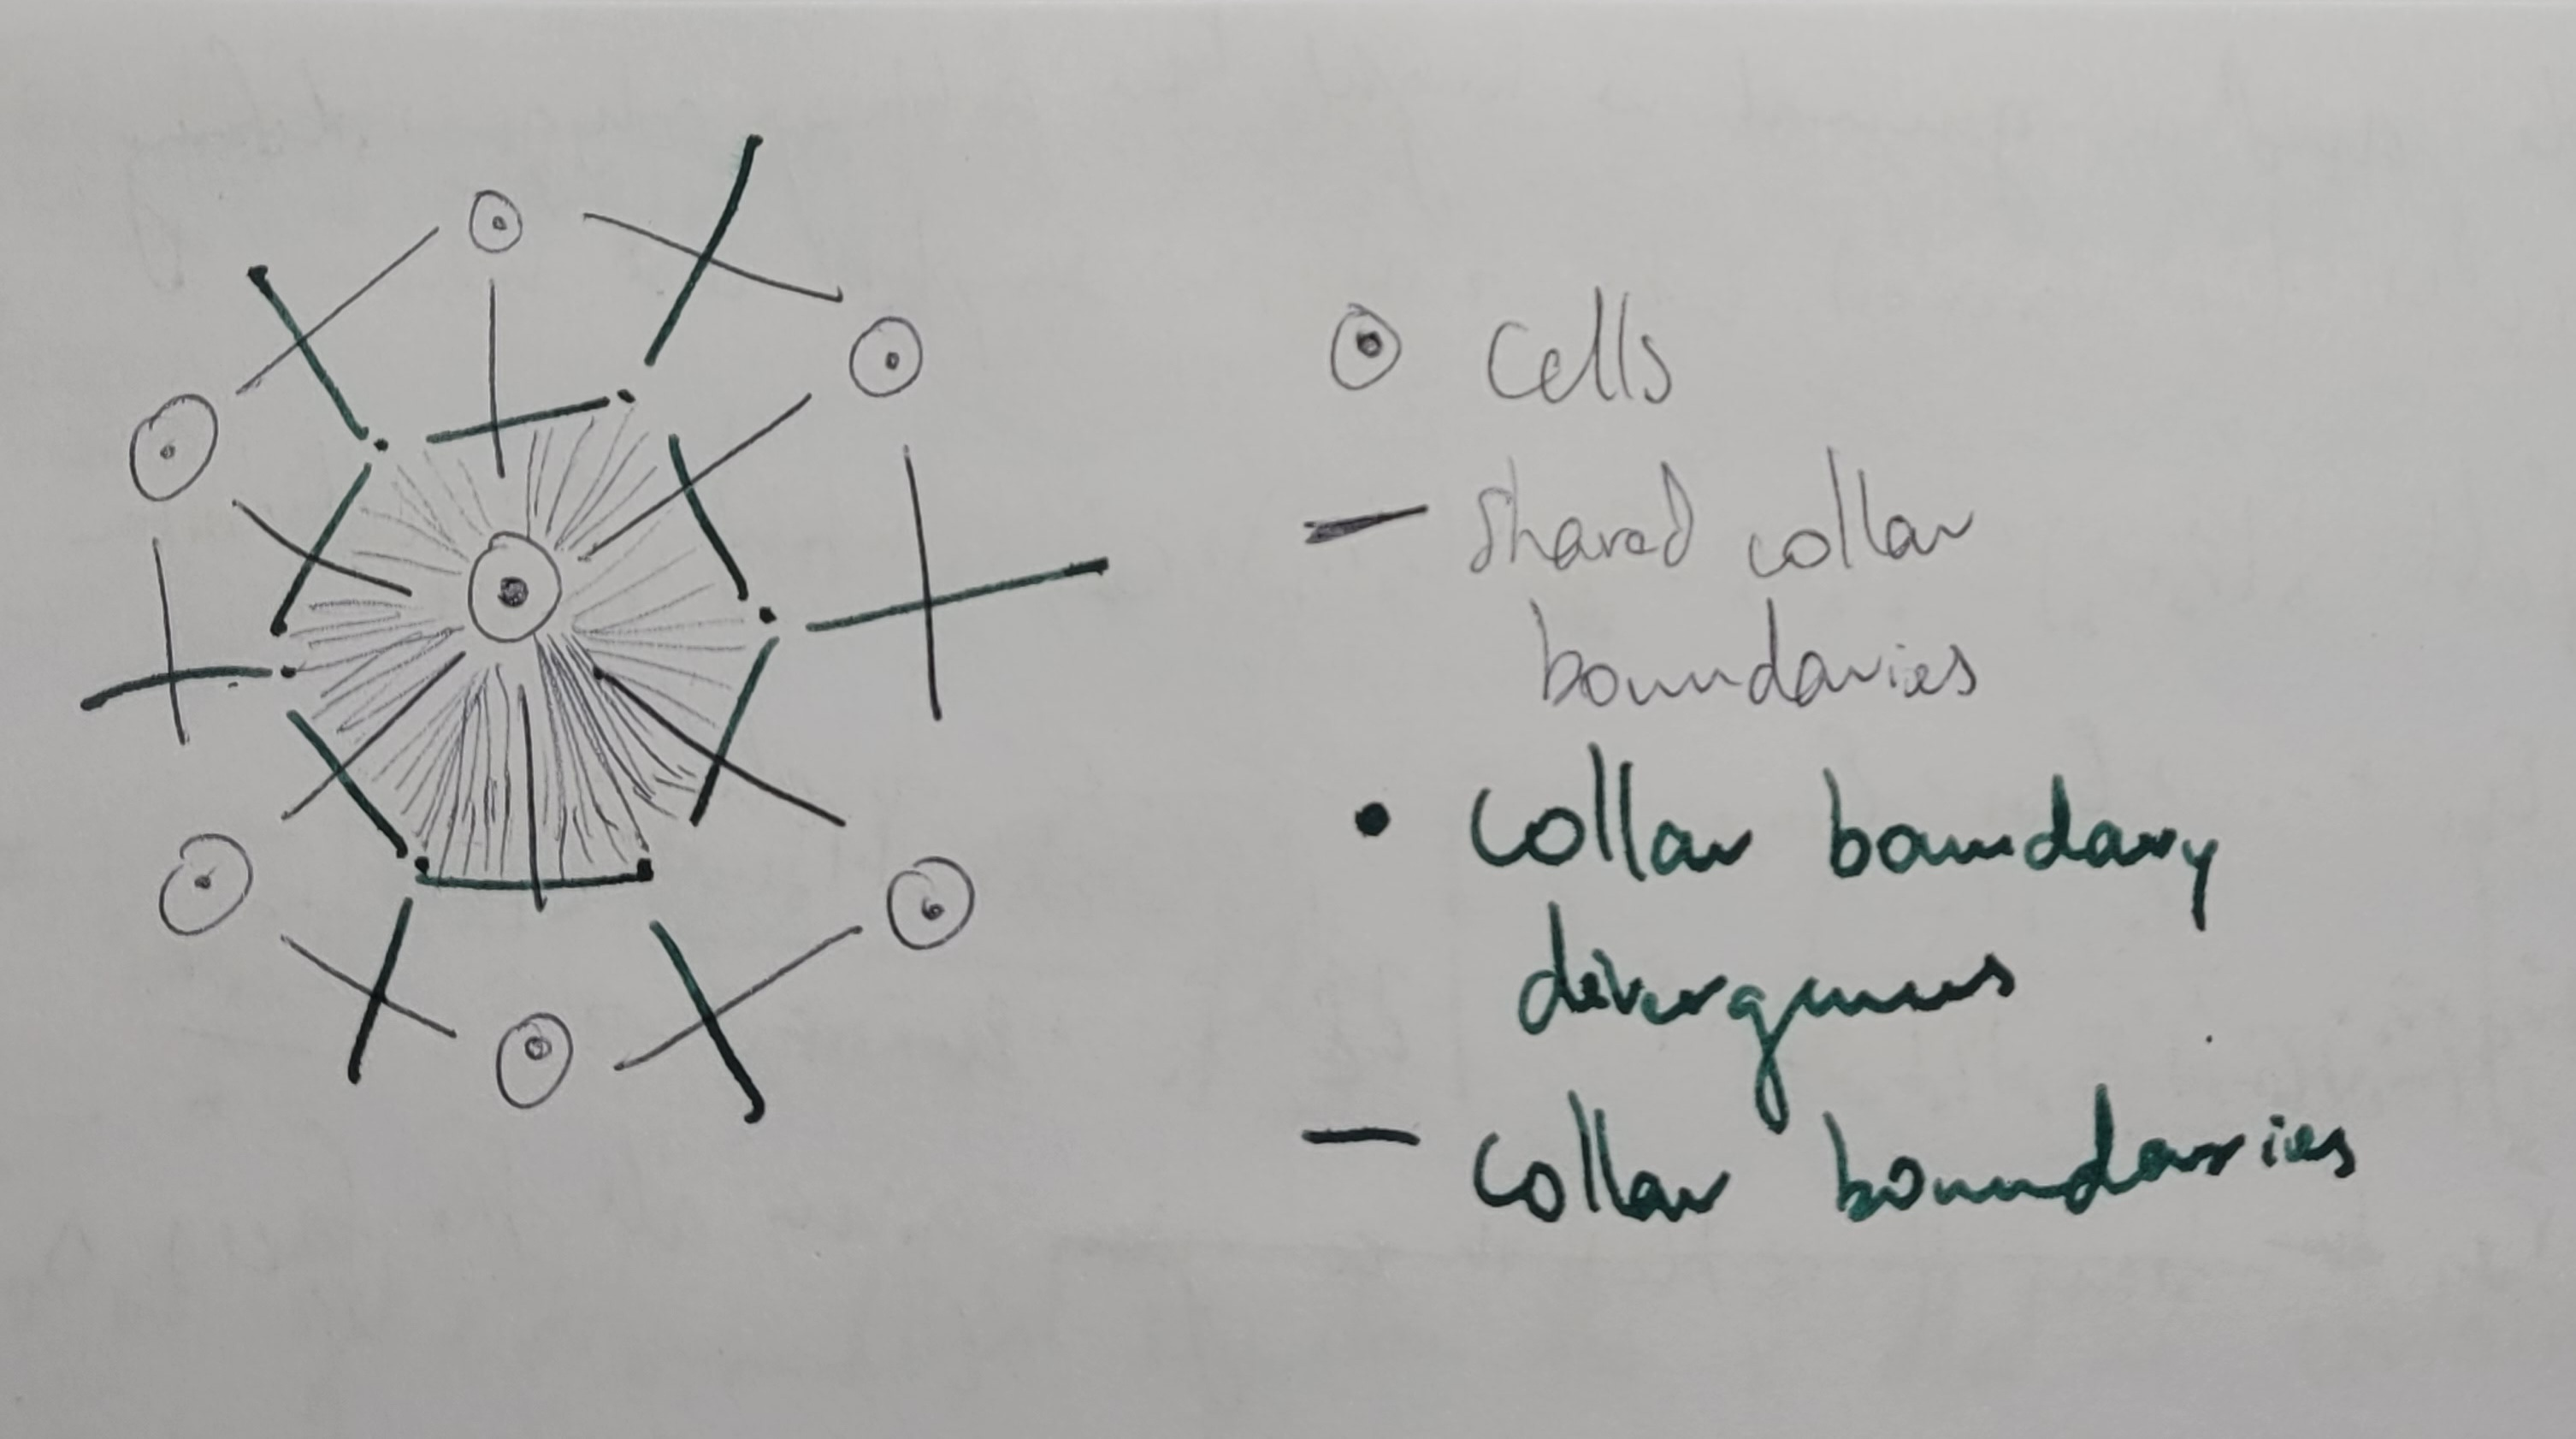
\includegraphics[width=\textwidth]{duals1.jpg}
        \caption{}
        \label{subfig:duals1}
    \end{subfigure}
    ~
    \begin{subfigure}[b]{0.46\textwidth}
        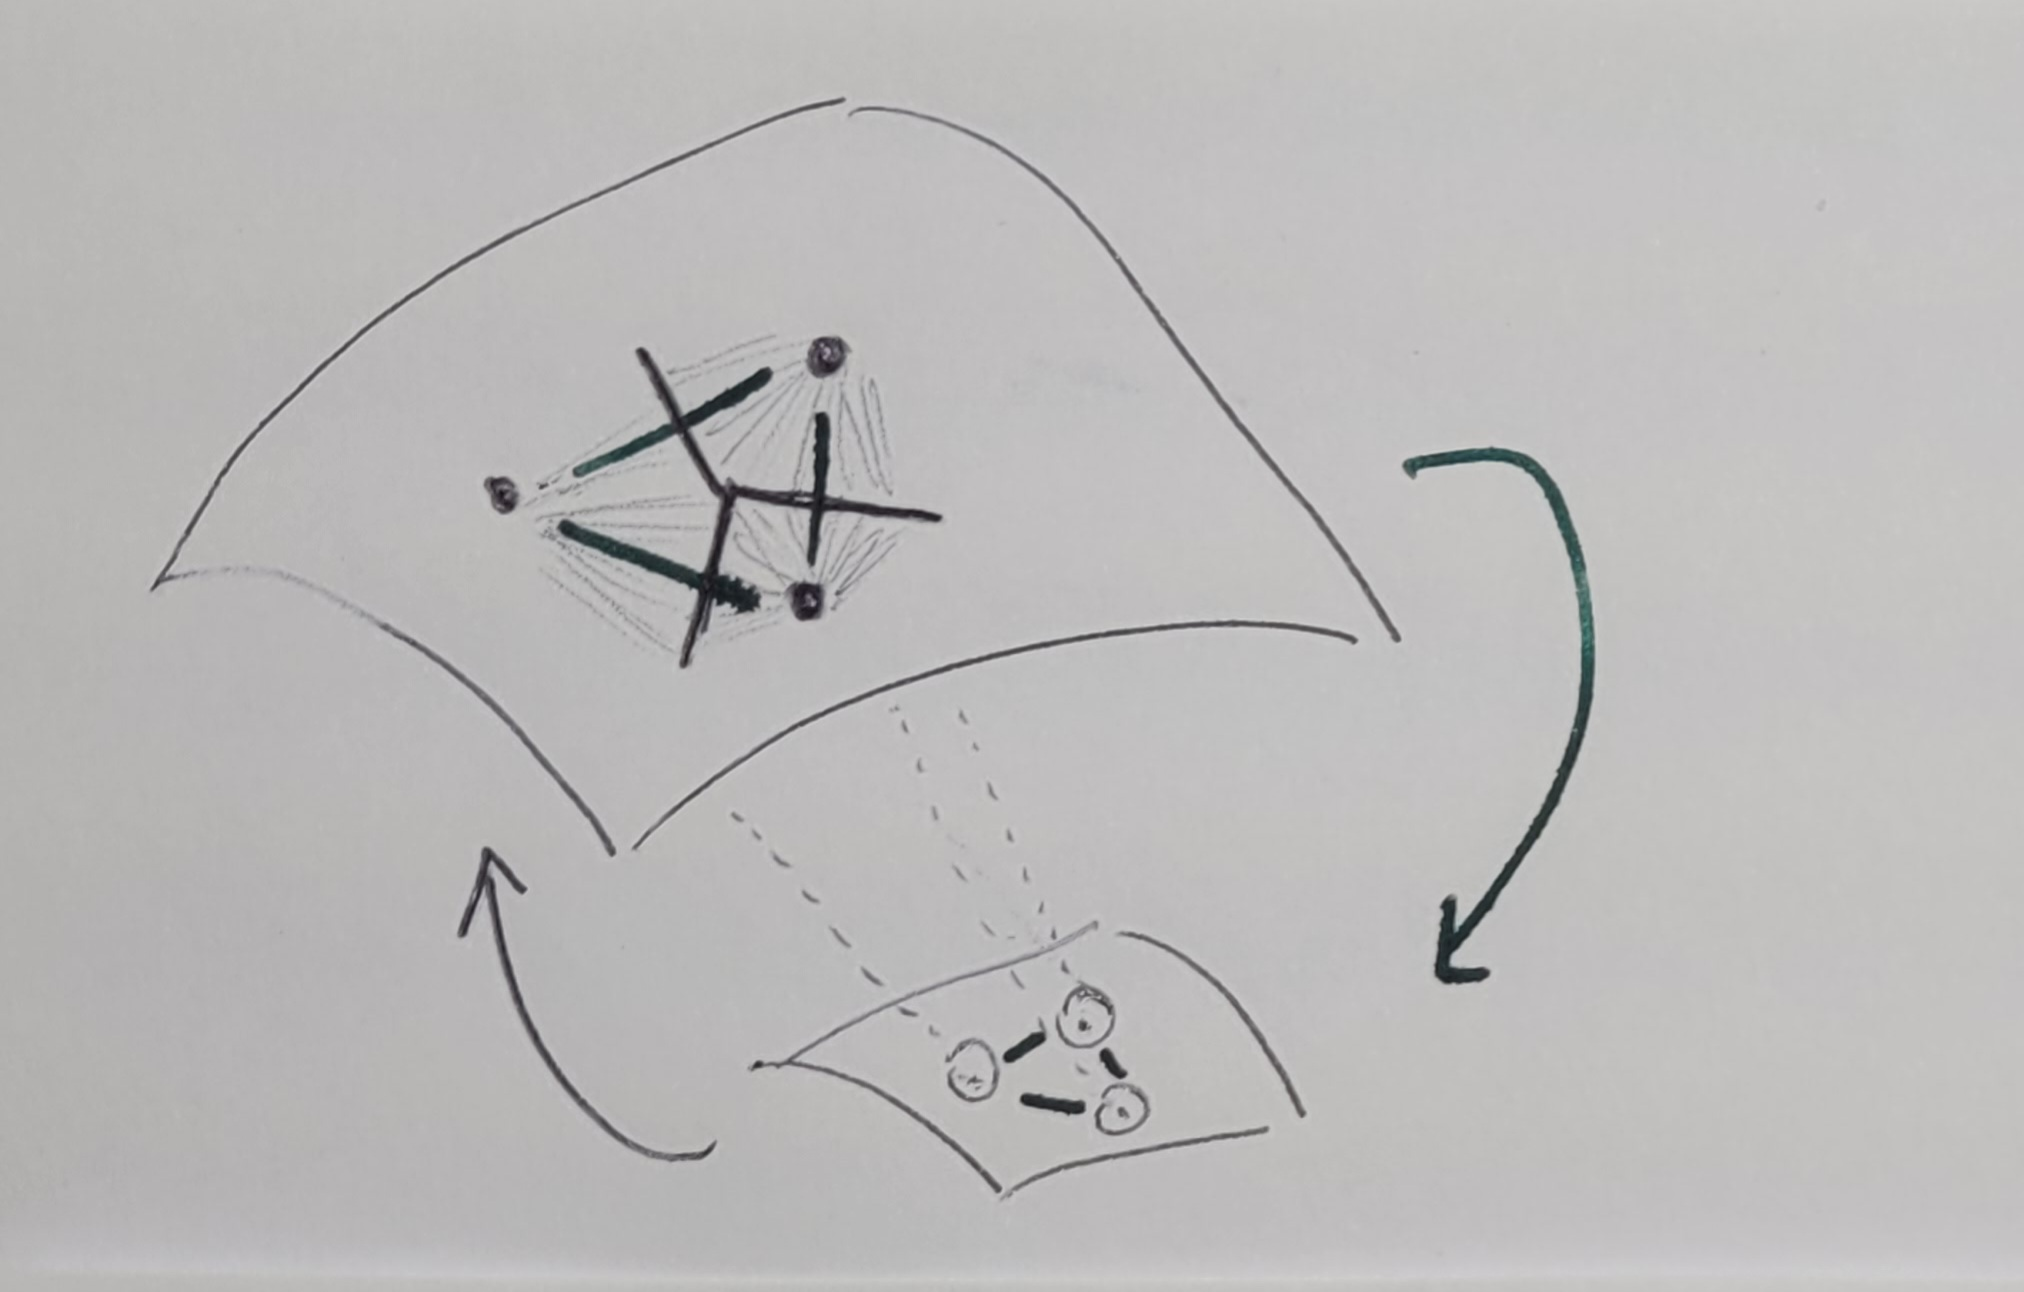
\includegraphics[width=\textwidth]{duals2.jpg}
        \caption{}
        \label{subfig:duals2}
    \end{subfigure}
    \caption{Two views of the physical dual graphs used in describing \textit{C. flexa}.}
    \label{fig:duals}
\end{figure}

\subsection{Surface formed by collar boundaries}
\subsubsection{Stretching}

The physical interactions happen at the collar boundaries, so it makes sense to define energy based on the graph that quantifies them. If two cells have a collar boundary described by $\bm{r_a} t + (1-t)\bm{r_b}$ with $0 \leq t \leq 1$ and the energy is defined by continuously many springs from the boundary to a projected cell point $\bm{r_\Delta}$, then the energy $\e_{ab}$ of that boundary is 

\begin{align}
    \e_{ab} = \int_0^1 \left[(\bm{r_a}t + (1-t)\bm{r_b}) - \bm{r_\Delta} \right]^2 dt &= \frac{1}{3} (\bm{r_a} + \bm{r_b})^2 - \frac{1}{3} \bm{r_a}\cdot\bm{r_b} - \bm{r_\Delta} \cdot (\bm{r_a} + \bm{r_b}) + \bm{r_\Delta}^2. \label{eq:eab}
\end{align}

The energy corresponding to a cell consists of the line energies of all the collar interfaces. We find the position $\bm{r_\Delta}$ by setting the gradient of equation \ref{eq:eab} with respect to $\bm{r_\Delta}$ to zero for all lines $ab$. If $b$ indexes the vertices that cell $\Delta$ has, then 

\begin{align*}
    0 = \frac{d\e}{d\bm{r_\Delta}} &= -\sum_{b\in\Delta} \bm{r_b} + 2n\bm{r_\Delta} \\
    \bm{r_\Delta} &= \frac{1}{n} \sum_{b\in\Delta} \bm{r_b}.
\end{align*}

The force on vertex $a$ is then given by the gradient of the whole sheet energy $\e_{\text{sheet}}$, which is the sum of the energies $\e_\Delta$ corresponding to each cell $\Delta$. 

\begin{align*}
    \frac{d \e_{\text{sheet}}}{d\bm{r_a}} &= \frac{d}{d\bm{r_a}} \sum_\Delta \e_\Delta = \sum_{\Delta:a \in \Delta} \frac{d\e_\Delta}{d\bm{r_a}} = \sum_{\Delta:a\in\Delta} \frac{d}{d\bm{r_a}} \sum_{b \in \Delta} (\bm{r_b} - \bm{r_\Delta})^2. \\
    \intertext{Since $\bm{r_\Delta}$ depends on $\bm{r_a}$ itself, we write} \\
    \bm{f_{\text{on }a}} &= -\sum_{\Delta:a\in\Delta} \frac{d}{d\bm{r_a}} \sum_{b \in \Delta} \left(\bm{r_b} - \frac{1}{n} \sum_{c\in\Delta} \bm{r_c} \right)^2 \\
    &= \sum_{\Delta:a\in\Delta} \sum_{b \in \Delta} \left(2\bm{r_a}\delta_{ab} - \frac{2}{n} \sum_{c\in\Delta}\left(\bm{r_c}\delta_{ab} + \bm{r_b}\delta_{ac}\right) + \frac{1}{n^2} \sum_{c\in\Delta}\sum_{d\in\Delta} \left(\delta_{ac}\bm{r_d} + \delta_{ad}\bm{r_c} \right) \right) \\
    &= -2\left(\bm{r_a} - \bm{r_\Delta} \right)
\end{align*}

This process was overkill, since we could have reasonably assumed that $\bm{r_\Delta}$ would be at the vertices' center of mass and that we'd effectively get springs from $\bm{r_\Delta}$ to each vertex. This is thanks to linearity of the collar springs. However, assuming that the collars have a positive equilibrium length $r_0$ makes it necessary to go through the above procedure.

If instead the line energy is 

\begin{align*}
    \e_{ab} &= \int_0^1 \left(\left|\bm{r_a}t + (1-t)\bm{r_b} - \bm{r_\Delta}\right| - r_0 \right)^2 dt, \\
    \intertext{then the cell position $\bm{r_\Delta}$ is the solution to} \\
    0 &= -2 \sum_{b\in\Delta} \bm{r_b} + 6 \bm{r_\Delta} - 2r_0 \frac{d}{d\bm{r_\Delta}} \sum_{(b,c) \text{ edge in }\Delta} \int_0^1 \left| \bm{r_b}t - (1-t)\bm{r_c} - \bm{r_\Delta} \right| dt \\
    0 &= -2 \sum_{b\in\Delta} \bm{r_b} + 6 \bm{r_\Delta} - 2r_0 \sum_{(b,c)} \int_0^1 \frac{\bm{r_\Delta} - \bm{r_c} - t(\bm{r_b} - \bm{r_c})}{\left|\bm{r_b}t - (1-t)\bm{r_c} - \bm{r_\Delta} \right|} dt.
\end{align*}

We can actually evaluate the integral above, but I found that it gives a transcendental equation for $\bm{r_\Delta}$ and decided it wasn't pursuing further on paper. Nonzero equilibrium length springs is better pursued numerically. Alternatively, we simply define springs from $\bm{r_\Delta}$ to each dual graph vertex rather than making the collars consist of continuous springs.

\subsubsection{Bending}

One way to define a bending energy is to give each cell a vector that corresponds to the midline pointing out from the center of the cell, which I have implicitly drawn in the figures of individuals flexas. From there, we could reasonably define a bending energy from the interactions between two interacting flexas by the angle between their corresponding ``normal'' vectors weighted by the length of their interface. 

Defining an individual vector is made complicated by the fact that the vertices along the cycles corresponding to each flexa are not necessarily coplanar, provided that a given cell is interacting with more than three other cells. One option, although I have not developed it, is to find the plane whose summed mean squared distances to each vertex for a cell is minimised. It would possibly be more accurate to again treat the edges as lines and minimise the integrated distance from the normal plane to the edges. Either way, the energy dictated by the angle between adjacent normal vectors will need to be summed over all pairs of neighboring cells, namely all edges in the graph where edges correspond to cell neighbors (not collar interfaces).

\subsection{Surface formed by cell bodies}

The graph of cell bodies and neighbor edges makes it easy to work with springs, but it is less clear how to define a bending energy. The math for springs is identical to previously, so let's just think about how to define bending energy.

\textbf{needs more work}

% \subsubsection{Bending}

\section{Including both cells and collar boundaries}

\subsection{Initial sheet}
Let's call the graph of cells with cell-cell neighbor relations as edges $G$, and the dual graph of collar boundaries $G^*$. For setting up the network topology, we proceed by defining $G$ to lie in the $xy$-plane with a set of cell coordinates $\{\bm{r}_c\}_{c\in C}$ for the set of cells $C$ and using Voronoi tessellation to build $G^*$. This is nice because it generalises beyond regular lattices. The curvature will be built in later when minimising the sheet energy.

We can build a super graph $\mathfrak{G}$ which has both the cell positions and collar boundaries, as well as edges from each cell $c$ to the boundary vertices $b$ in the cell's set of collar boundary vertices $B_c \in V^*$. That is, $\mathfrak{G}$ has the cell-cell neighbor edges $E$ between cell vertices $C$, collar vertices $V^*$, and edges $\{ \{(c, b)\}_{b\in B_c} \}_{c\in C}$. 

Since Voronoi regions for cells that aren't completely surrounded by other cells (which I will call \textit{boundary cells}) extend out to infinity, we need to create a new vertex at each infinite boundary to make a finite collar boundary. (Figure \ref{fig:voronoi})

\begin{figure}[htbp]
    \centering
    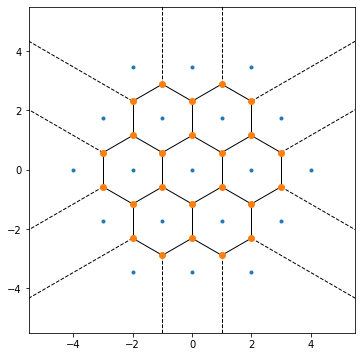
\includegraphics[width=0.5\textwidth]{voronoi.png}
    \caption{Voronoi tesselation of initial cell placement. Cell bodies shown in blue points, collar boundaries shown in black lines with collar boundary end points shown in orange. Notably, the regions corresponding to boundary cells extend out to infinity. We need to add all boundary collar vertices along the infinite dashed lines.}
    \label{fig:voronoi}
\end{figure}

\subsubsection{Why do boundary collar vertices matter?}

Does it matter that boundary cells have collar nodes at the boundary? We can answer this analytically. For cells $a, c$ and mutual interior collar boundary vertex $b$, suppose the physically finite collar boundary ends at point $\bm{r}$. We want to know how the angle between the planes $\bm{r}_a, \bm{r}_b, \bm{r}$ and $\bm{r}_c, \bm{r}_b, \bm{r}$ changes as $\bm{r}$ changes. 

For now let's say that the collar length is fixed as $\ell$, so the range of motion of $\bm{r}$ is constrained. We can simplify our problem by reparameterising our coordinates such that $\bm{r}_a = (-1, 0, 0)$, $\bm{r}_b = (0, r, 0)$, and $\bm{r}_c = (1, 0, 0)$, where $r = \sqrt{\ell^2 - 1}$. Note that $\ell$ is a dimensionless ratio of the collar length to cell-cell distance here.\footnote{Later we will use $\ell$ as the only length scale in the problem when we're solving the sheet shape by minimising energy.} It is easy to show that the solution set for allowable values of $\bm{r}$ is given by solutions satisfying $r^2 = y^2 + z^2$, $x=0$. Equivalently, the possible vectors $\bm{r}(\theta)$ are $(0, r\cos\theta, r\sin\theta)$. So let's find the normal vectors between the two collar-cell-collar surfaces to see if the plane-plane angle changes with $\theta$. 

We have the normals are 
\begin{align*}
    \hat{\bm{n}}_1 &= (\bm{r} - \bm{r}_a) \times (\bm{r}_b - \bm{r}_a) \\
    &= \frac{(-r^2 \sin\theta, r\sin\theta, r - r\cos\theta)}{r^4\sin^2\theta + 2r^2(1-\cos\theta)} \\
    \hat{\bm{n}}_2 &= (\bm{r}_b - \bm{r}_c) \times (\bm{r} - \bm{r}_c)\\
    &= \frac{(r^2 \sin\theta, r\sin\theta, r\cos\theta - r)}{r^4\sin^2\theta + 2r^2(1-\cos\theta)}.
\end{align*}
\noindent Their angle is given by (after simplifying)
\begin{align*}
    \hat{\bm{n}}_1 \cdot \hat{\bm{n}}_2 &= 1 - \frac{2}{1 + \frac{1}{2r^2} \left(1+\tan^2\frac{\theta}{2}\right)}.
\end{align*}

The point is that the plane-plane angle changes with $\theta$! So the boundary collar nodes really have an effect on the sheet energy, and we need to include them. This is an important result too since (as Lloyd always reminds me) the boundary conditions affect the whole shape of the sheet. So one way to conceivably move the sheet is by updating the boundary collar nodes then working inward to update the whole sheet shape. 

Regardless, this tells us that we need to add our own boundary collar nodes to our simulation, since they aren't provided by the Voronoi tessellation.

\subsubsection{Adding boundary collar vertices}

The coordinate system for each cell-cell neighbor pair we developed in the previous section is useful for creating our own new boundary collar vertices. For two boundary cell positions $\bm{r}_{c_1}, \bm{r}_{c_2}$, we can take the orthogonal component of $\bm{r}_{b} - \bm{r}_{c_1}$ (where $b$ is the existing collar boundary node between $c_1, c_2$) with respect to $\bm{r}_{c_1} - \bm{r}_{c_2}$. Adding this orthogonal component to the cells' center of mass $(\bm{r}_{c_1} + \bm{r}_{c_2})/2$ (which is on the Voronoi boundary) will give a new position equidistant from the two cells, where the cell-collar lengths is the same as that to the existing collar boundary vertex. 

\begin{figure}[hbtp]
    \centering
    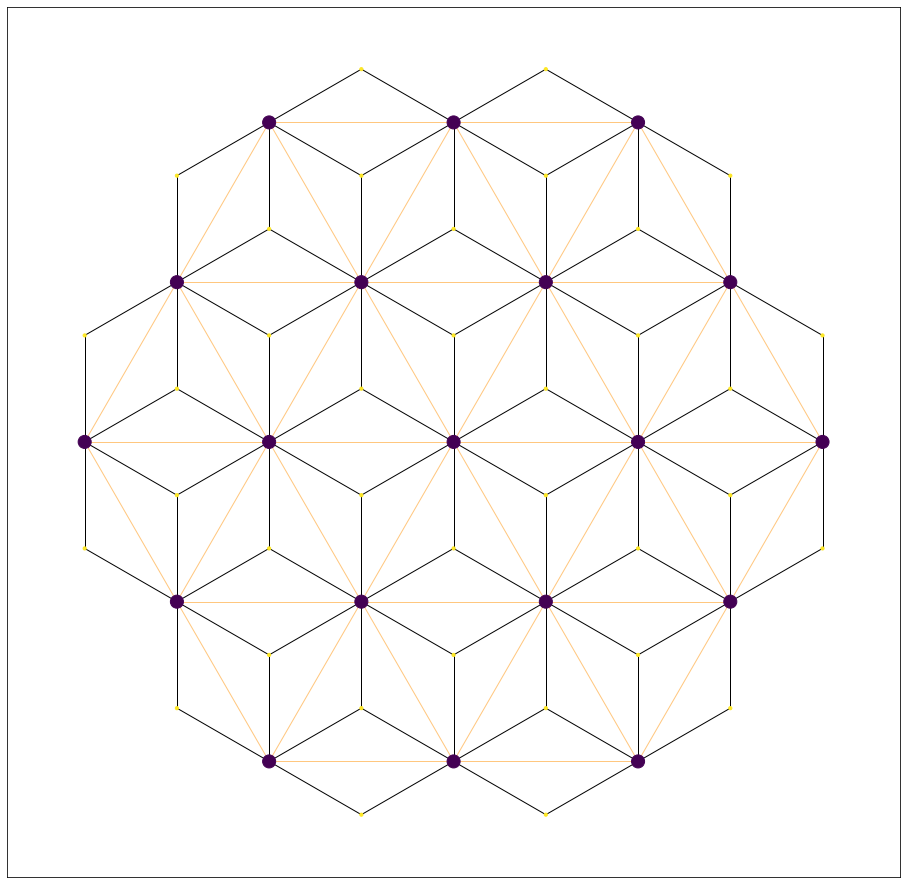
\includegraphics[width=0.8\textwidth]{layout_init.png}
    \caption{Initial layout for the flexa sheet. Cell bodies are shown in large purple points and collar boundary vertices are shown in small yellow points. Black edges connect cells to collar boundary vertices, and orange edges show cell-cell neighbor relations (though these orange edges are not physically present). The physical interactions are mediated through the black edges.}
    \label{fig:layout_init}
\end{figure}

The resulting cell sheet and collar boundary surface is shown in Figure \ref{fig:layout_init}. Notice in particular that every cell on the boundary has two collar nodes between it and its neighboring cells on the boundary. This whole graph $\mathfrak{G}$ is shown projected onto the $xy$-plane, but the collar interactions are all offset in $z$ relative to the cells. 

\subsection{Bending energies}

\subsubsection{Collar length}
For now, we are going to take the collar lengths to be fixed at their initial lengths. Since we're using a regular lattice for now, we can define this as $\ell$ to be the only length in our problem. (Cell-cell distance will change when we minimise the energy.)

Later, it would be nice to add a collar length energy term $(|\bm{r}_c - \bm{r}_{b_{c}}| - r_0)^2$ term that makes the cell-collar lengths flexible.

\subsubsection{Cell-collar angle $\phi$ energy}

The paper we're basing our work on defines the collar angle $\phi$ relative to the direction of the cell body $\hat{n}_c$ for cell $c$. Immediately, we run into a problem, which is that $\hat{n}$ is not clearly defined when the cell is interacting with several other cells. When that happens, the cell's collar does not necessarily form its boundaries in a plane. 

\paragraph{Defining the cell normal vector $\hat{n}_c$}
We can define the cell's vector $\hat{n}_c$ for a cell $c$ by taking the average vector from $\bm{r}_c$ to $\bm{r}_b$ for all collar boundary nodes $b \in B_c$. However, we run into a problem for boundary cells, which is that this normal vector then points inward towards the sheet because we didn't define collar boundary nodes that don't connect to other cells. In the language of Figure \ref{fig:layout_init}, the boundary cells have less than a symmetric set of 6 collar boundary nodes. 

This doesn't agree with our intuition, since the entire sheet is flat. So we expect the cells at the boundaries to have vectors $\hat{n}_c$ pointing directly in $+\hat{\bm{z}}$ (as the collars are above the cell sheet in $z$). Instead, we can define $\hat{n}_c$ by taking a plane approximation to the collar boundary position vectors $\{ \bm{r}_b \}_{b \in B_c}$. This plane defines a normal vector.

If we approximate $\hat{z}_b = (x_b, y_b)\cdot (\beta_1, \beta_2) + \beta_0$ and minimize the sum of squared residuals $\sum_{b\in B_c} (\hat{z}_b - z_b)^2$ with respect to $\beta_0, \beta_1, \beta_2$,\footnote{We do this with ordinary least squares, which is why I use the notation $\hat{z}_b$ and $\bm{\beta}$.} then the normal vector of the plane approximation is $(\beta_1, \beta_2, -1)$ up to normalisation and multiplication by $-1$. 

We need to orient the cell's vector $\hat{\bm{n}}_c$ so that it points in the direction from the cell to the collar. Fortunately, we could use the average cell-to-collar vector that we discussed before to do this alignment. 

\paragraph{What is the best normal vector for a cell?}

Suppose a cell is at position $\bm{r}_c$ with collar vertices at $\bm{r}_b$ for $b \in B_c$. We can ask how the cell orients itself to minimise its collar energy in $\phi$. The energy of the cell $\e_c$ is given by 

\begin{align*}
    \e_c &= \sum_{b\in B_c} \left[ \arccos\left(\frac{\bm{r}_b - \bm{r}_c}{\left|\bm{r}_b - \bm{r}_c\right|} \cdot \hat{n}_c \right) - \phi_0 \right]^2. \\
    \intertext{We can ask what normal vector minimises $\e_c$ by setting the gradient of $\e_c$ with respect to $\hat{\bm{n}}_c$ to zero. But the length of $\hat{\bm{n}}_c$ is fixed at one, so we solve } \\
    0 &= \frac{\partial \left[ \e_c + \lambda\left( \left| \hat{\bm{n}}_c\right|^2 - 1\right) \right] }{\partial \hat{\bm{n}}_c} \\
    \intertext{subject to $\left| \hat{\bm{n}}_c\right|^2 = 1$. I found that } \\
    \lambda \hat{\bm{n}}_c &= 2 \sum_{b \in B_c} \left[ \arccos\left(\frac{\bm{r}_b - \bm{r}_c}{\left|\bm{r}_b - \bm{r}_c\right|} \cdot \hat{n}_c \right) - \phi_0 \right] \frac{-1}{\sqrt{1 - \left(\frac{\bm{r}_b - \bm{r}_c}{\left|\bm{r}_b - \bm{r}_c\right|} \cdot \hat{n}_c \right)^2 }}\frac{\bm{r}_b - \bm{r}_c}{\left|\bm{r}_b - \bm{r}_c\right|}
    \\
    \lambda &= 2 \left| \sum_{b\in B_c} \left[\arccos\left(\frac{\bm{r}_b - \bm{r}_c}{\left|\bm{r}_b - \bm{r}_c\right|} \cdot \hat{n}_c \right) - \phi_0 \right]
    \frac{1}{\sqrt{1 - \left(\frac{\bm{r}_b - \bm{r}_c}{\left|\bm{r}_b - \bm{r}_c\right|} \cdot \hat{n}_c \right)^2 }}
    \frac{\bm{r}_b - \bm{r}_c}{\left|\bm{r}_b - \bm{r}_c\right|} \right|. \\
    \intertext{Then } \\
    \hat{\bm{n}}_c &= \frac{\sum_{b \in B_c} \left[ \arccos\left(\frac{\bm{r}_b - \bm{r}_c}{\left|\bm{r}_b - \bm{r}_c\right|} \cdot \hat{n}_c \right) - \phi_0 \right] \frac{-1}{\sqrt{1 - \left(\frac{\bm{r}_b - \bm{r}_c}{\left|\bm{r}_b - \bm{r}_c\right|} \cdot \hat{n}_c \right)^2 }}\frac{\bm{r}_b - \bm{r}_c}{\left|\bm{r}_b - \bm{r}_c\right|}}{\left| \sum_{b'\in B_c} \left[\arccos\left(\frac{\bm{r}_{b'} - \bm{r}_c}{\left|\bm{r}_{b'} - \bm{r}_c\right|} \cdot \hat{n}_c \right) - \phi_0 \right]
    \frac{1}{\sqrt{1 - \left(\frac{\bm{r}_{b'} - \bm{r}_c}{\left|\bm{r}_{b'} - \bm{r}_c\right|} \cdot \hat{n}_c \right)^2 }}
    \frac{\bm{r}_{b'} - \bm{r}_c}{\left|\bm{r}_{b'} - \bm{r}_c\right|} \right|}
\end{align*}



\paragraph{Calculating collar angle $\phi$}
Once we have a cell normal vector $\hat{n}_c$ for each cell $c$, it is easy to calculate the collar angles $\phi_{cb}$ to each collar boundary vertex $b\in B_c$. Now, indexing over all cell-collar edges in $\mathfrak{G}$ (black edges in Figure \ref{fig:layout_init}), we write the $\phi$ energy
\begin{align*}
    \e_\phi &= \sum_{c\in C} \sum_{b \in B_c} (\phi_{cb} - \phi_0)^2 = \sum_{(c,b) \in \{\text{cell-collar edges }(c,b) \}} (\phi_{cb} - \phi_0)^2.
\end{align*}

When $\phi_0$ is equal to the initial angle between $\hat{\bm{z}}$ (which is the initial $\hat{n}_c$ for each cell $c$) and each cell-collar vector $\bm{r}_b - \bm{r}_c$ (which is well-defined because we're using a regular lattice to start), we get that $\e_\phi=0$ numerically. This confirms that our code is calculating the energy right. Of course this energy will be nonzero when $\phi_0$ differs from the initial angle. 

\subsubsection{Cell-cell junction angle $\psi$ energy}

We suppose that there is also an energy $\e_\psi$ based on the angle $\psi$ that two cells make at their mutual collar boundary. We can calculate this as we did previously, where we found that the length of collar boundary (equivalently, the angle $\theta$ between the two collar nodes and each cell) affects the cell-collar-cell angle. Let's say there's an equilibrium angle $\psi_0$ between two cell collars.

For cells $c_1, c_2$ and mutual collar boundary vertices $b, b'$, we define $\hat{\bm{n}}_1$ and $\hat{\bm{n}}_2$ as the normal vectors to planes defined by $\bm{r}_{c_1}, \bm{r}_b, \bm{r}_{b'}$ and $\bm{r}_{c_2}, \bm{r}_b, \bm{r}_{b'}$. The angle between these planes is given as $\hat{\bm{n}}_1 \cdot \hat{\bm{n}}_2$, and the acute angle on the interior of the hinge is $\pi - \arccos \left( \hat{\bm{n}}_1 \cdot \hat{\bm{n}}_2 \right)$. 

Let's assume that the angle $\psi$ is shared evenly between the two cells, so that the cell $c_1$ contribution to $\e_\psi$ is $(\psi_{c_1, c_2} / 2 - \psi_0/2)^2$ for cell-cell neighbor relation $(c_1, c_2)$. Likewise for $c_2$. Then $\e_\psi$ indexes over the cell-cell neighbor relations in edge set $E$:

\begin{align*}
    \e_\psi &= \sum_{(c_1, c_2) \in E} (\psi_{c_1, c_2} / 2 - \psi_0/2)^2.
\end{align*}

\subsubsection{Flat sheet as a solution} \label{subsubsec:flat}

Notice that we have a pair $(\phi_0, \psi_0)$ that gives $\e = \e_\phi + \e_\psi = 0$. Since the $\phi$ and $\psi$ energies are nonnegative, the flat sheet is a stable minimum. 

\subsection{Minimising sheet energy}

We now have an energy $\e\{ \bm{r}_v \}_{v \in \mathfrak{G}} = \e_\phi + \e_\psi$ which is parameterised over the cell and collar boundary vertex positions. Notably, we treat the topology of the network as fixed, so the indices of the summations for $\e_\phi$ and $\e_\psi$ are unchanged even as we minimise energy.

\subsubsection{Constant collar length constraint}

For now, we are numerically constraining the cell-collar lengths at $\ell$, their initial lengths (which are constant for all cells). If we want to use the generalisability of our model to use an random initial cell distribution and generate the irregular boundaries with Voronoi tesselation, we will have to relax this condition and add a collar length spring energy to $\e$. The constant collar length constraint only applies to sheets generated by regular lattices when laid flat on a plane.

The constraint is defined by a vector function $f((c, b)) = |\bm{r}_c - \bm{r}_b| - \ell = 0$ for all cell-collar edges $(c, b)$. If $n_{\text{collars}}$ is the number of cell-collar edges in $\{\text{cell-collar edges }(c,b) \}$, then $f$ defines a $n_{\text{collars}}$-vector function. 

My optimisation routine requires that we calculate a Jacobian matrix for the vector constraint function. This gets ugly if we use $f$ as written above, but it is fortunately equivalent to set the constraint $f'((c, b)) = |\bm{r}_c - \bm{r}_b|^2 - \ell^2 = 0$. It is an interesting problem to take the gradient of $\bm{f'}$ with respect to all of the coordinates, but I won't include it here. It's implemented in my code.

\subsection{Numerical optimisation routine}

Finally, we numerically optimise. I changed $\phi_0$ to be defined relative to the initial value of $\phi$, and likewise for $\psi$. If we make $\phi_0$ smaller and $\psi_0$ larger, we expect the cell collars to contract and for cell-cell distances to lengthen. In other words, we expect the sheet to curve upward, so that the cells on the edges go in the direction that the collars are.

The numerical optimisation problem gives a clean sensible solution, which is shown projected onto the $xy$-plane in Figure \ref{fig:layout_curved}. We can tell that the sheet is curved just looking at this alone, which is a massive relief and confirmation of what we expect.

\begin{figure}[htbp]
    \centering
    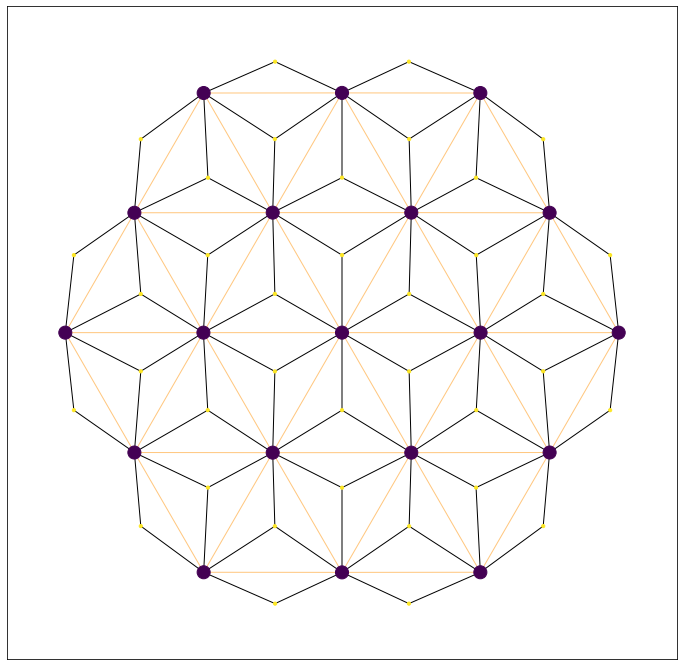
\includegraphics[width=0.8\textwidth]{layout_curved.png}
    \caption{Figure in the same style of Figure \ref{fig:layout_init} showing the cell sheet projected onto the $xy$-plane after minimising energy. }
    \label{fig:layout_curved}
\end{figure}

The solution in Figure \ref{fig:layout_curved} is for $\phi_0 = 0.99 \phi_{\text{init}}$ and $\phi_0 = 1.03 \psi_{\text{init}}$, where $\phi_{\text{init}}$ and $\psi_{\text{init}}$ are the initial angles in the flat sheet state. We could now bask in the glory of our solution and look at it in 3d (Figure \ref{subfig:shallow}).

The resulting structure is really pretty sensitive to small changes in $\phi_0, \psi_0$. Figure \ref{subfig:deep} shows the structure that comes out of $\phi_0 = 0.9 \phi_{\text{init}}$, $\psi_0 = 1.15\psi_{\text{init}}$. 

\begin{figure}[htbp]
    \centering
    \begin{subfigure}[b]{\textwidth}
        \centering 
        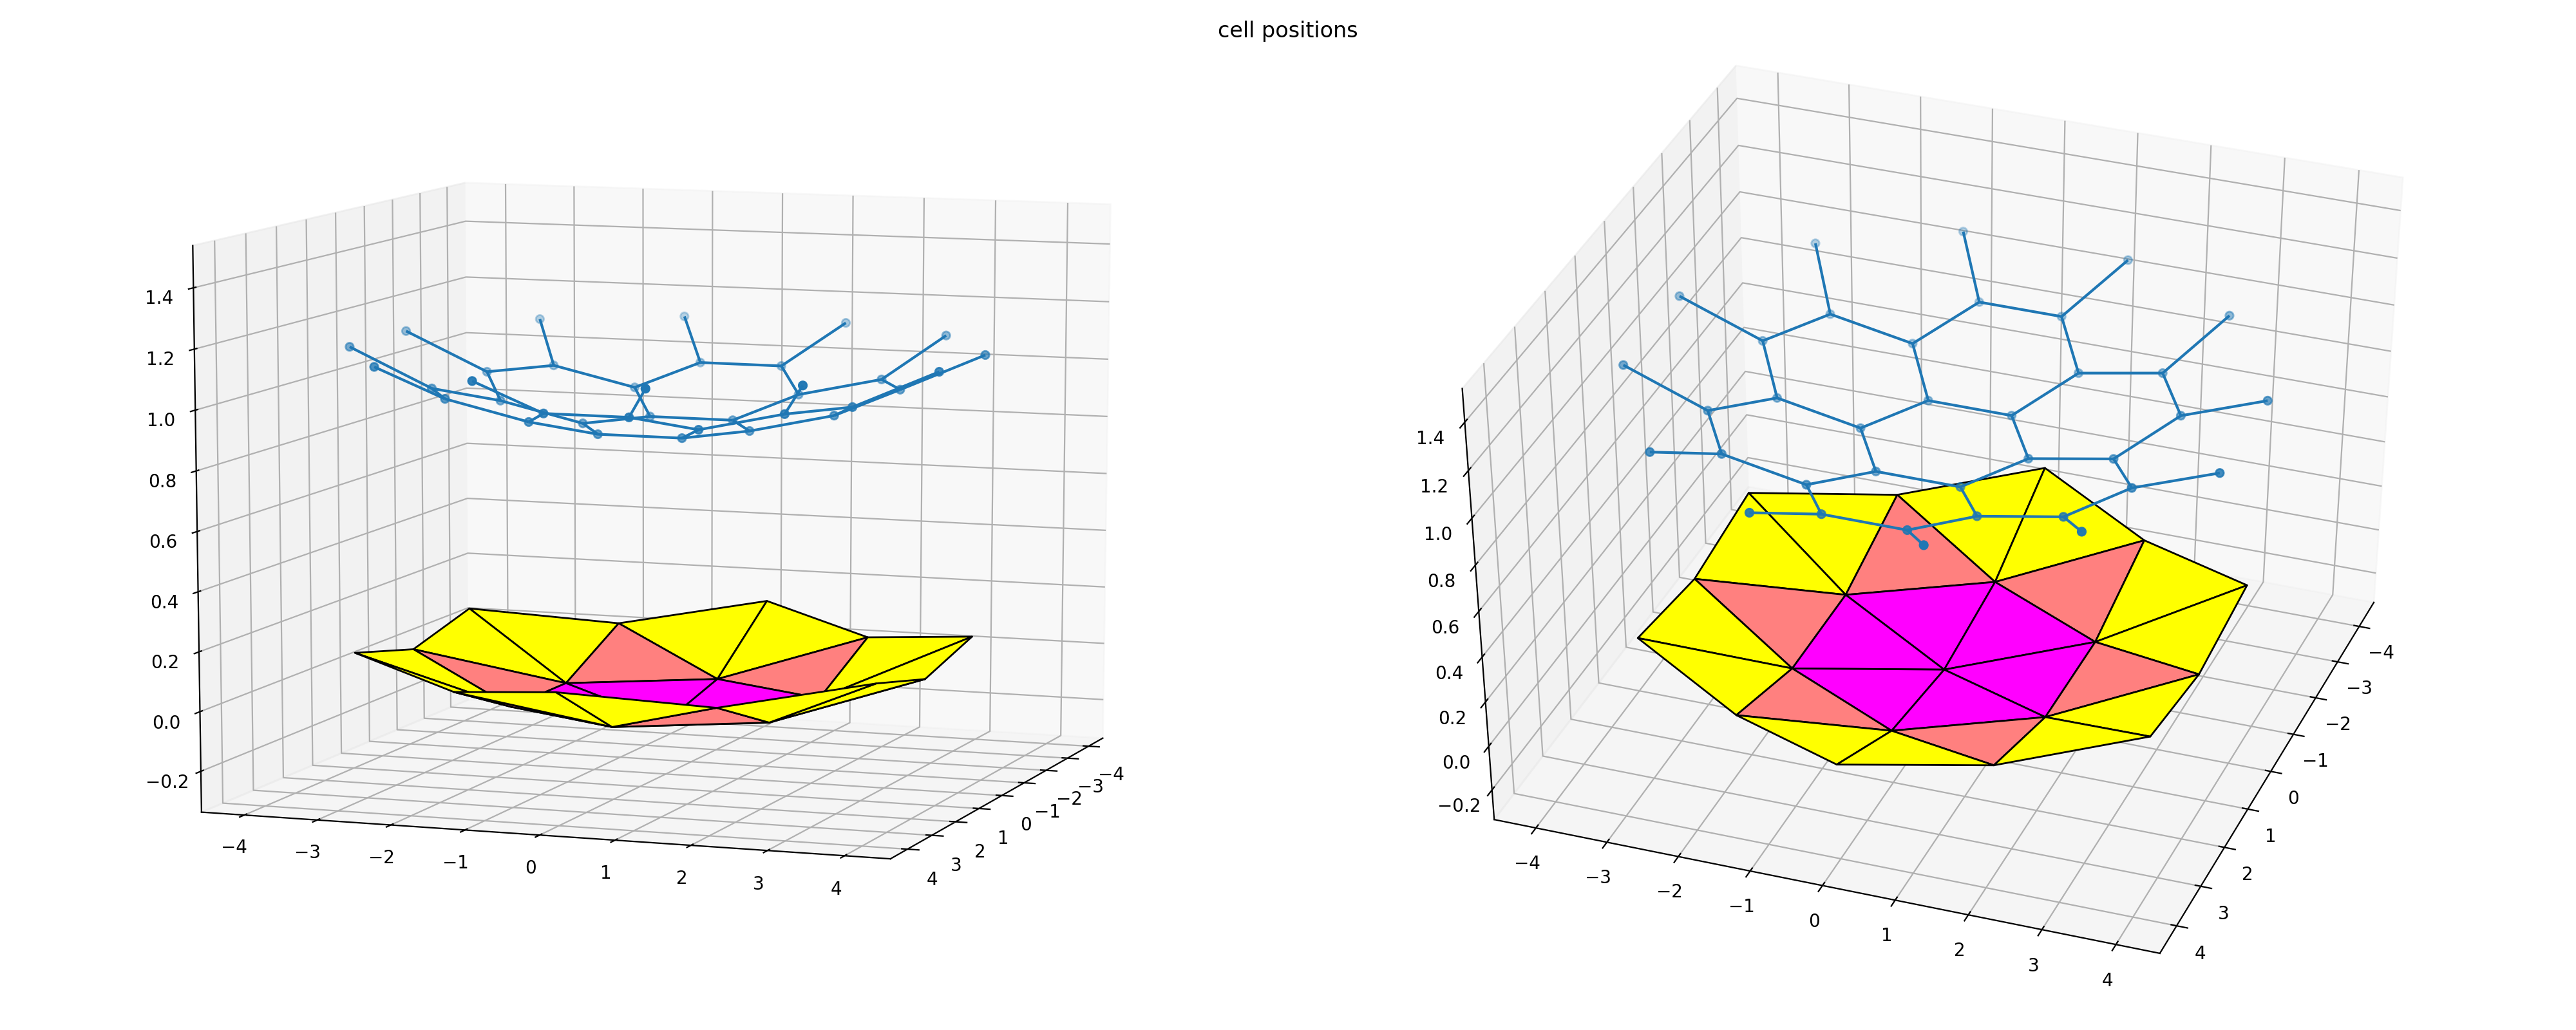
\includegraphics[width=\textwidth]{shallow.png}
        \caption{}
        \label{subfig:shallow}
    \end{subfigure}
    \begin{subfigure}[b]{\textwidth}
        \centering
        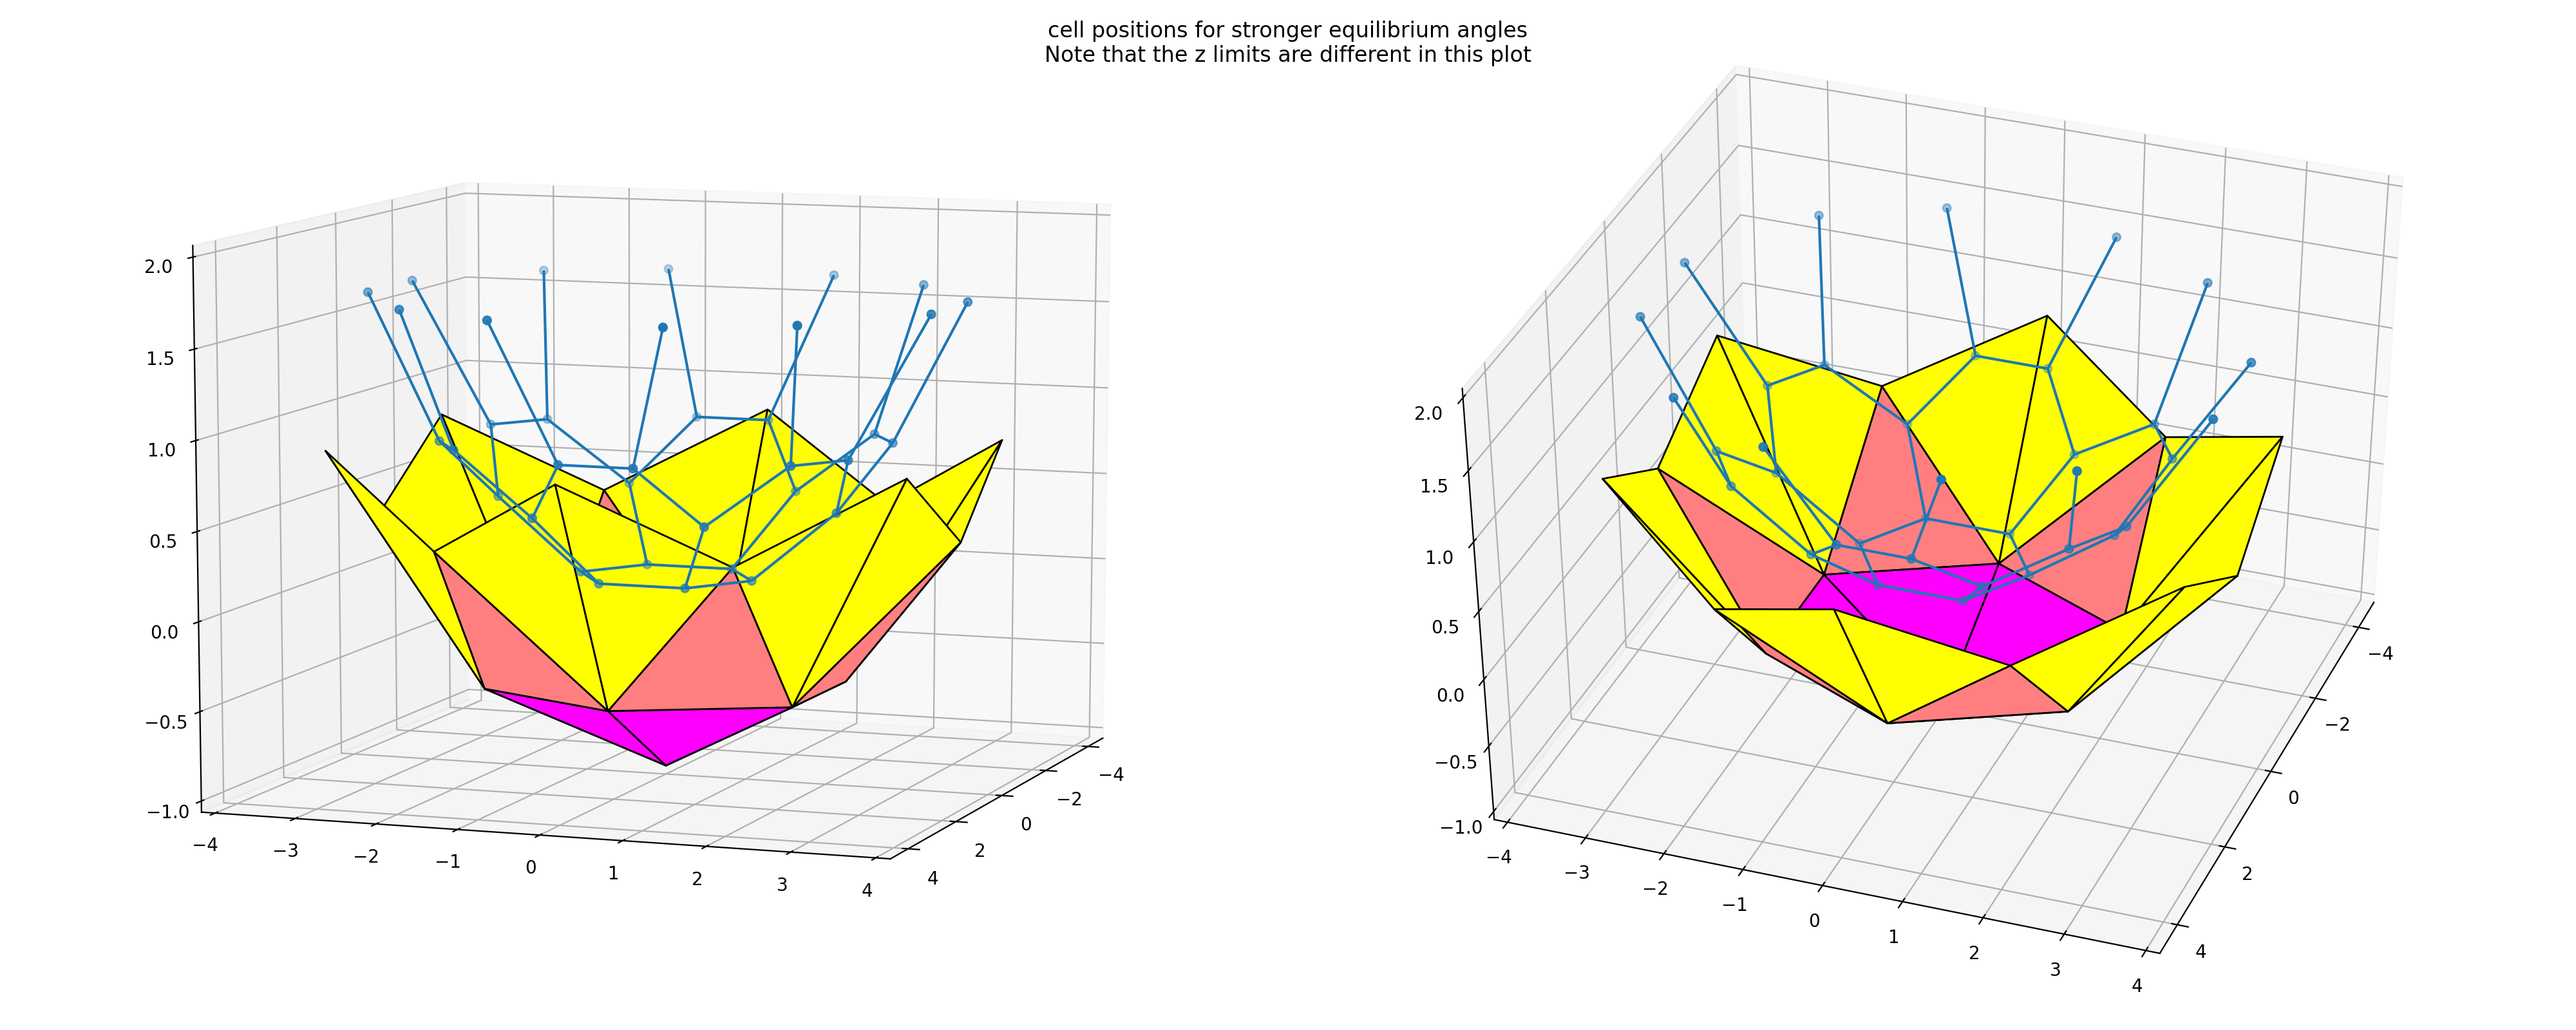
\includegraphics[width=\textwidth]{deep.png}
        \caption{3d projections of the curved sheet formed by $\phi_0 = 0.9 \phi_{\text{init}}$, $\psi_0 = 1.15\psi_{\text{init}}$. }
        \label{subfig:deep}
    \end{subfigure}
    \caption{Cell sheet geometry from the hexagonal lattice in Figure \ref{fig:layout_init} and parameters (\ref{subfig:shallow}) $\phi_0 = 0.99 \phi_{\text{init}}$, $\phi_0 = 1.03 \psi_{\text{init}}$, $\ell_0 = \ell_{\text{init}}=1.52$, (\ref{subfig:deep}) $\phi_0 = 0.9 \phi_{\text{init}}$, $\psi_0 = 1.15\psi_{\text{init}}$, $\ell_0 = \ell_{\text{init}}=1.52$. }
\end{figure}

\subsection{Topology}

In section \ref{subsubsec:flat}, I mentioned that the flat sheet is a stable minimum. But it is here because the lattice is regular. A single pentagon in a hexagonal lattice (like a football (soccer) ball, thanks Lloyd) will make it so no $\phi_0$ and $\psi_0$ will make every cell make the other cells flat. 

What I think is interesting about this is the connection between graph topology and surface geometry. I think, in a continuous sense, graph topology affects Gaussian curvature through the energy function. 

\subsubsection{Adding noise to initial cell positions in Figure \ref{fig:layout_init}}

We expect the initial lattice in Figure \ref{fig:layout_init} to produce a sheet with 6-fold symmetry. Since the graph of connections is produced by a Voronoi tessellation, small changes to initial boundary cell positions can change the graph topology for boundary cells. 

When adding noise to the initial cell positions, the change in topology at some boundary nodes results in substantial effects felt over the sheet. Figure \ref{fig:hexnoise} shows the effect of different topology at the boundary.

\begin{figure}[htbp]
    \centering
    \begin{subfigure}[b]{\textwidth}
        \centering
        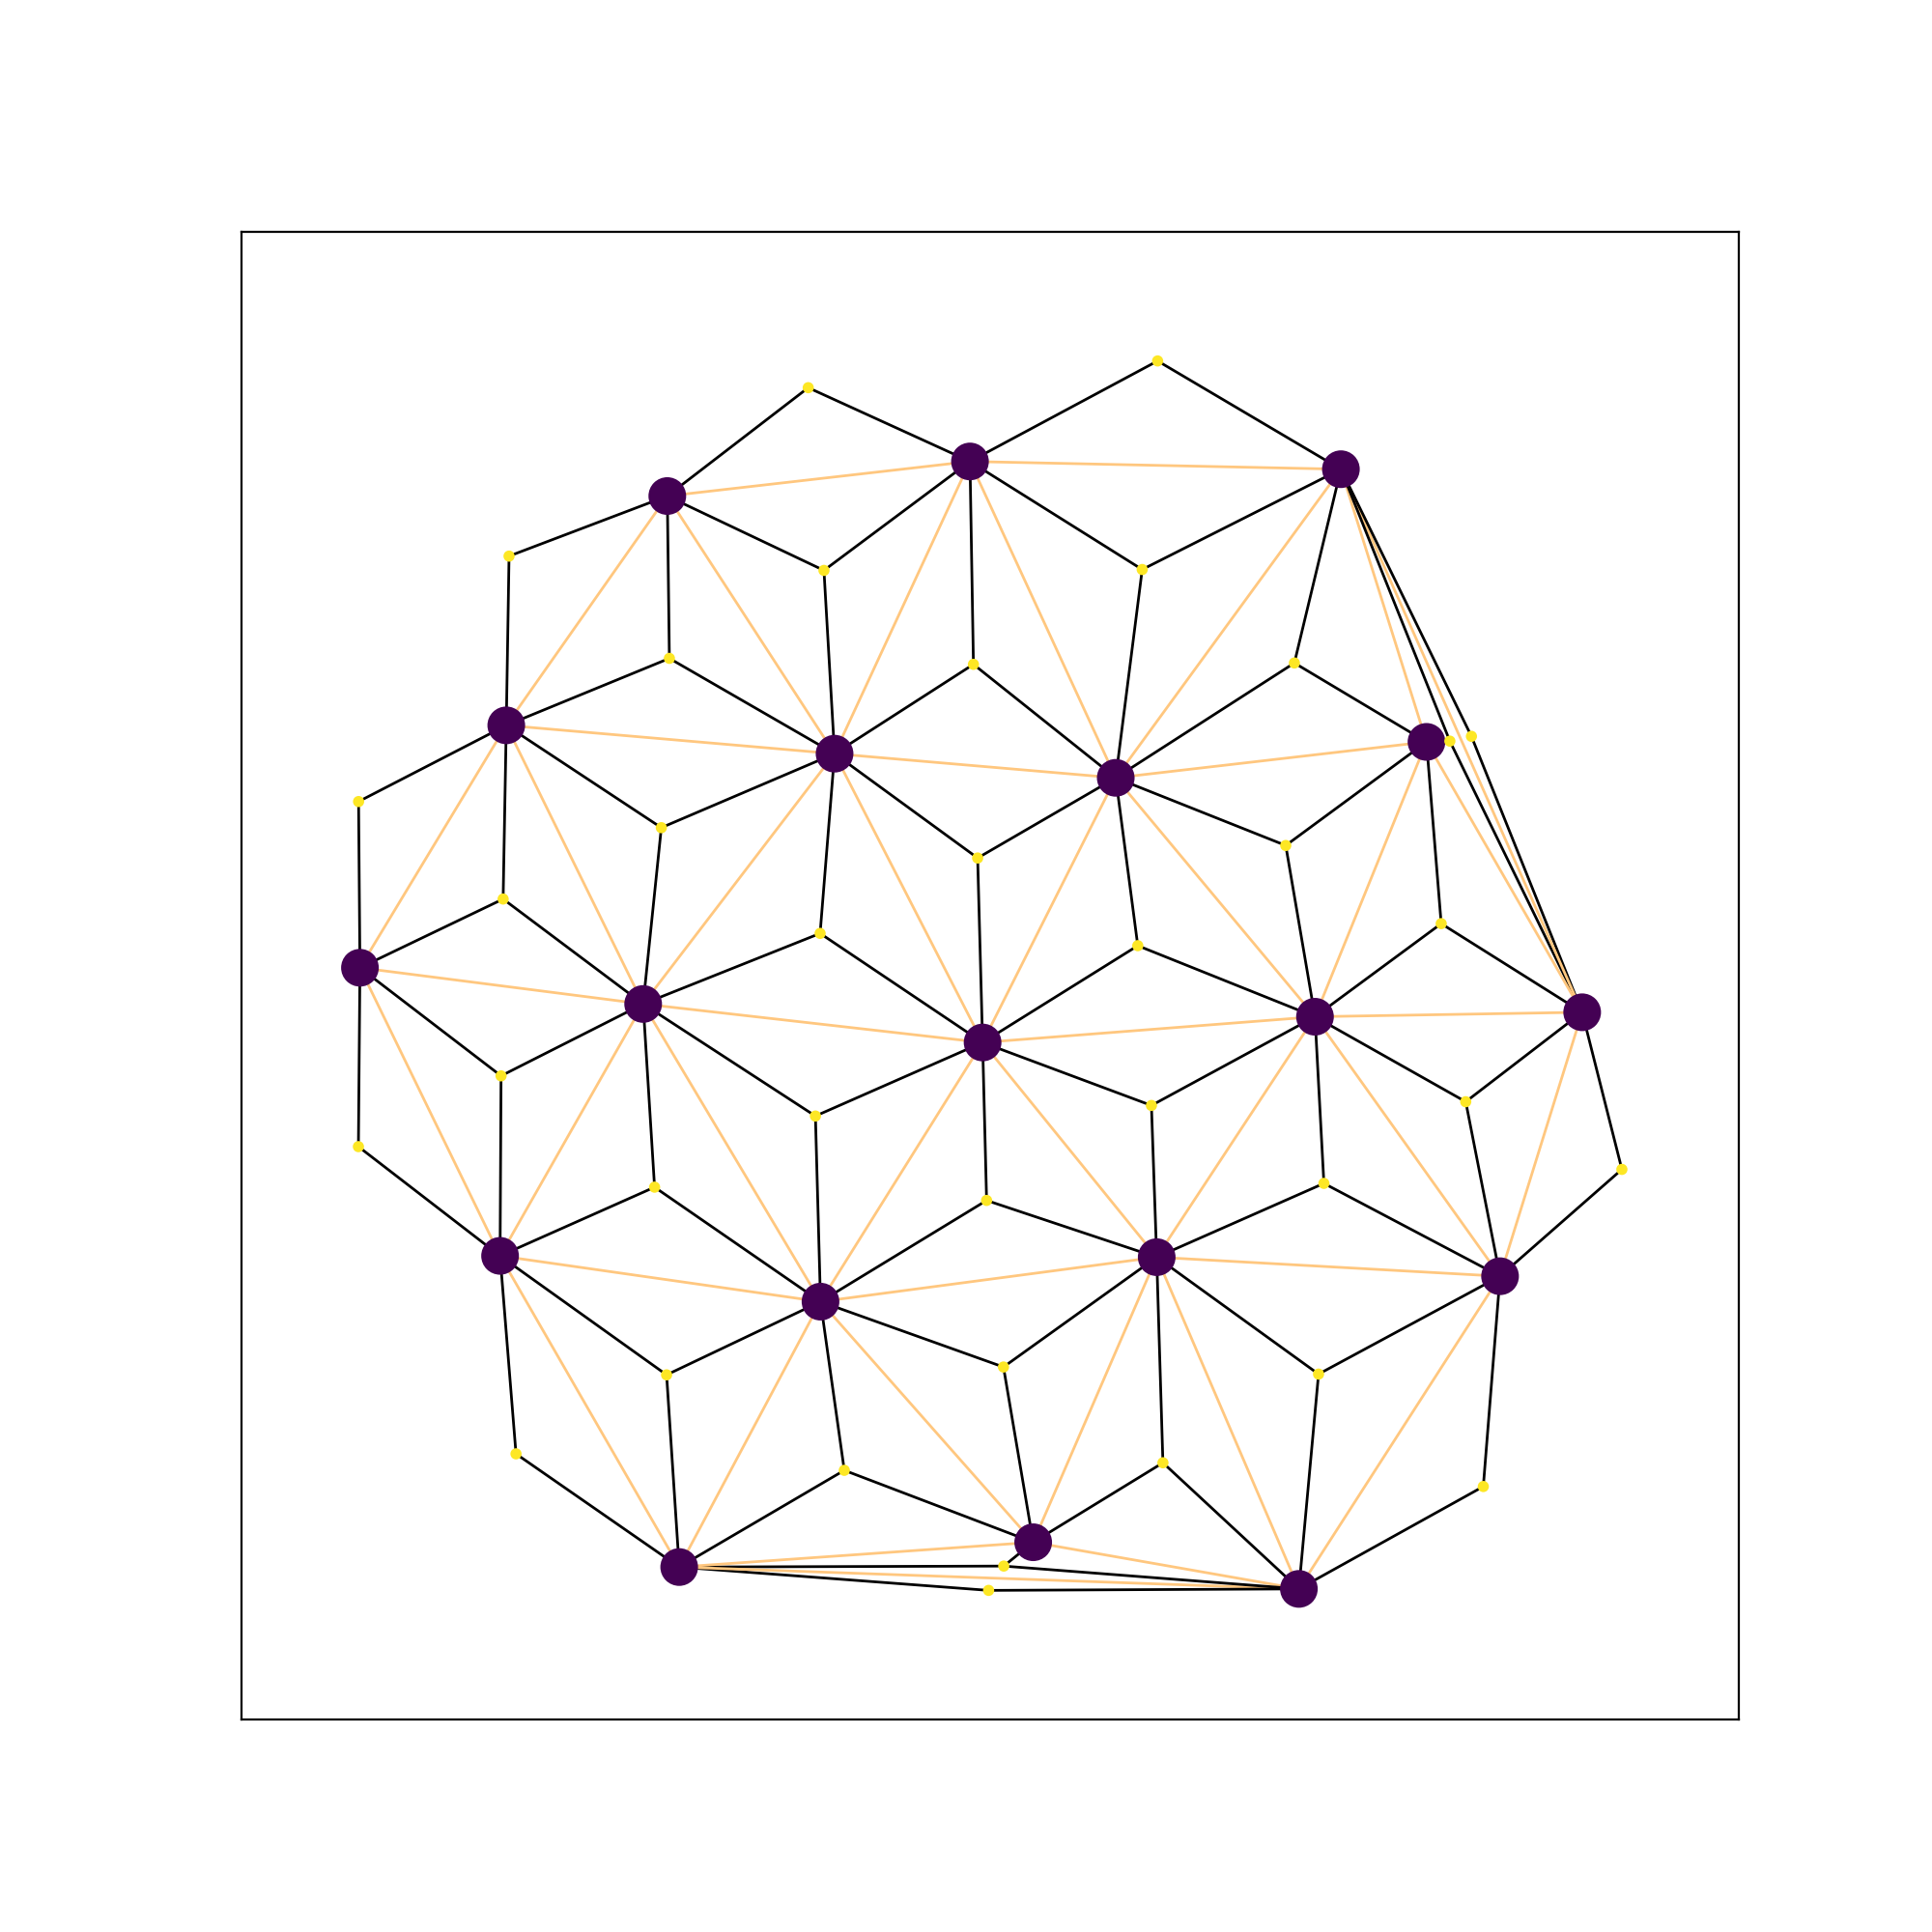
\includegraphics[width=0.5\textwidth]{hexnoise/hexnoise_graph.png}
        \caption{Initial lattice drawn as in Figure \ref{fig:layout_init}.}
        \label{subfig:hexnoise_graph}
    \end{subfigure}
    \begin{subfigure}[b]{\textwidth}
        \centering
        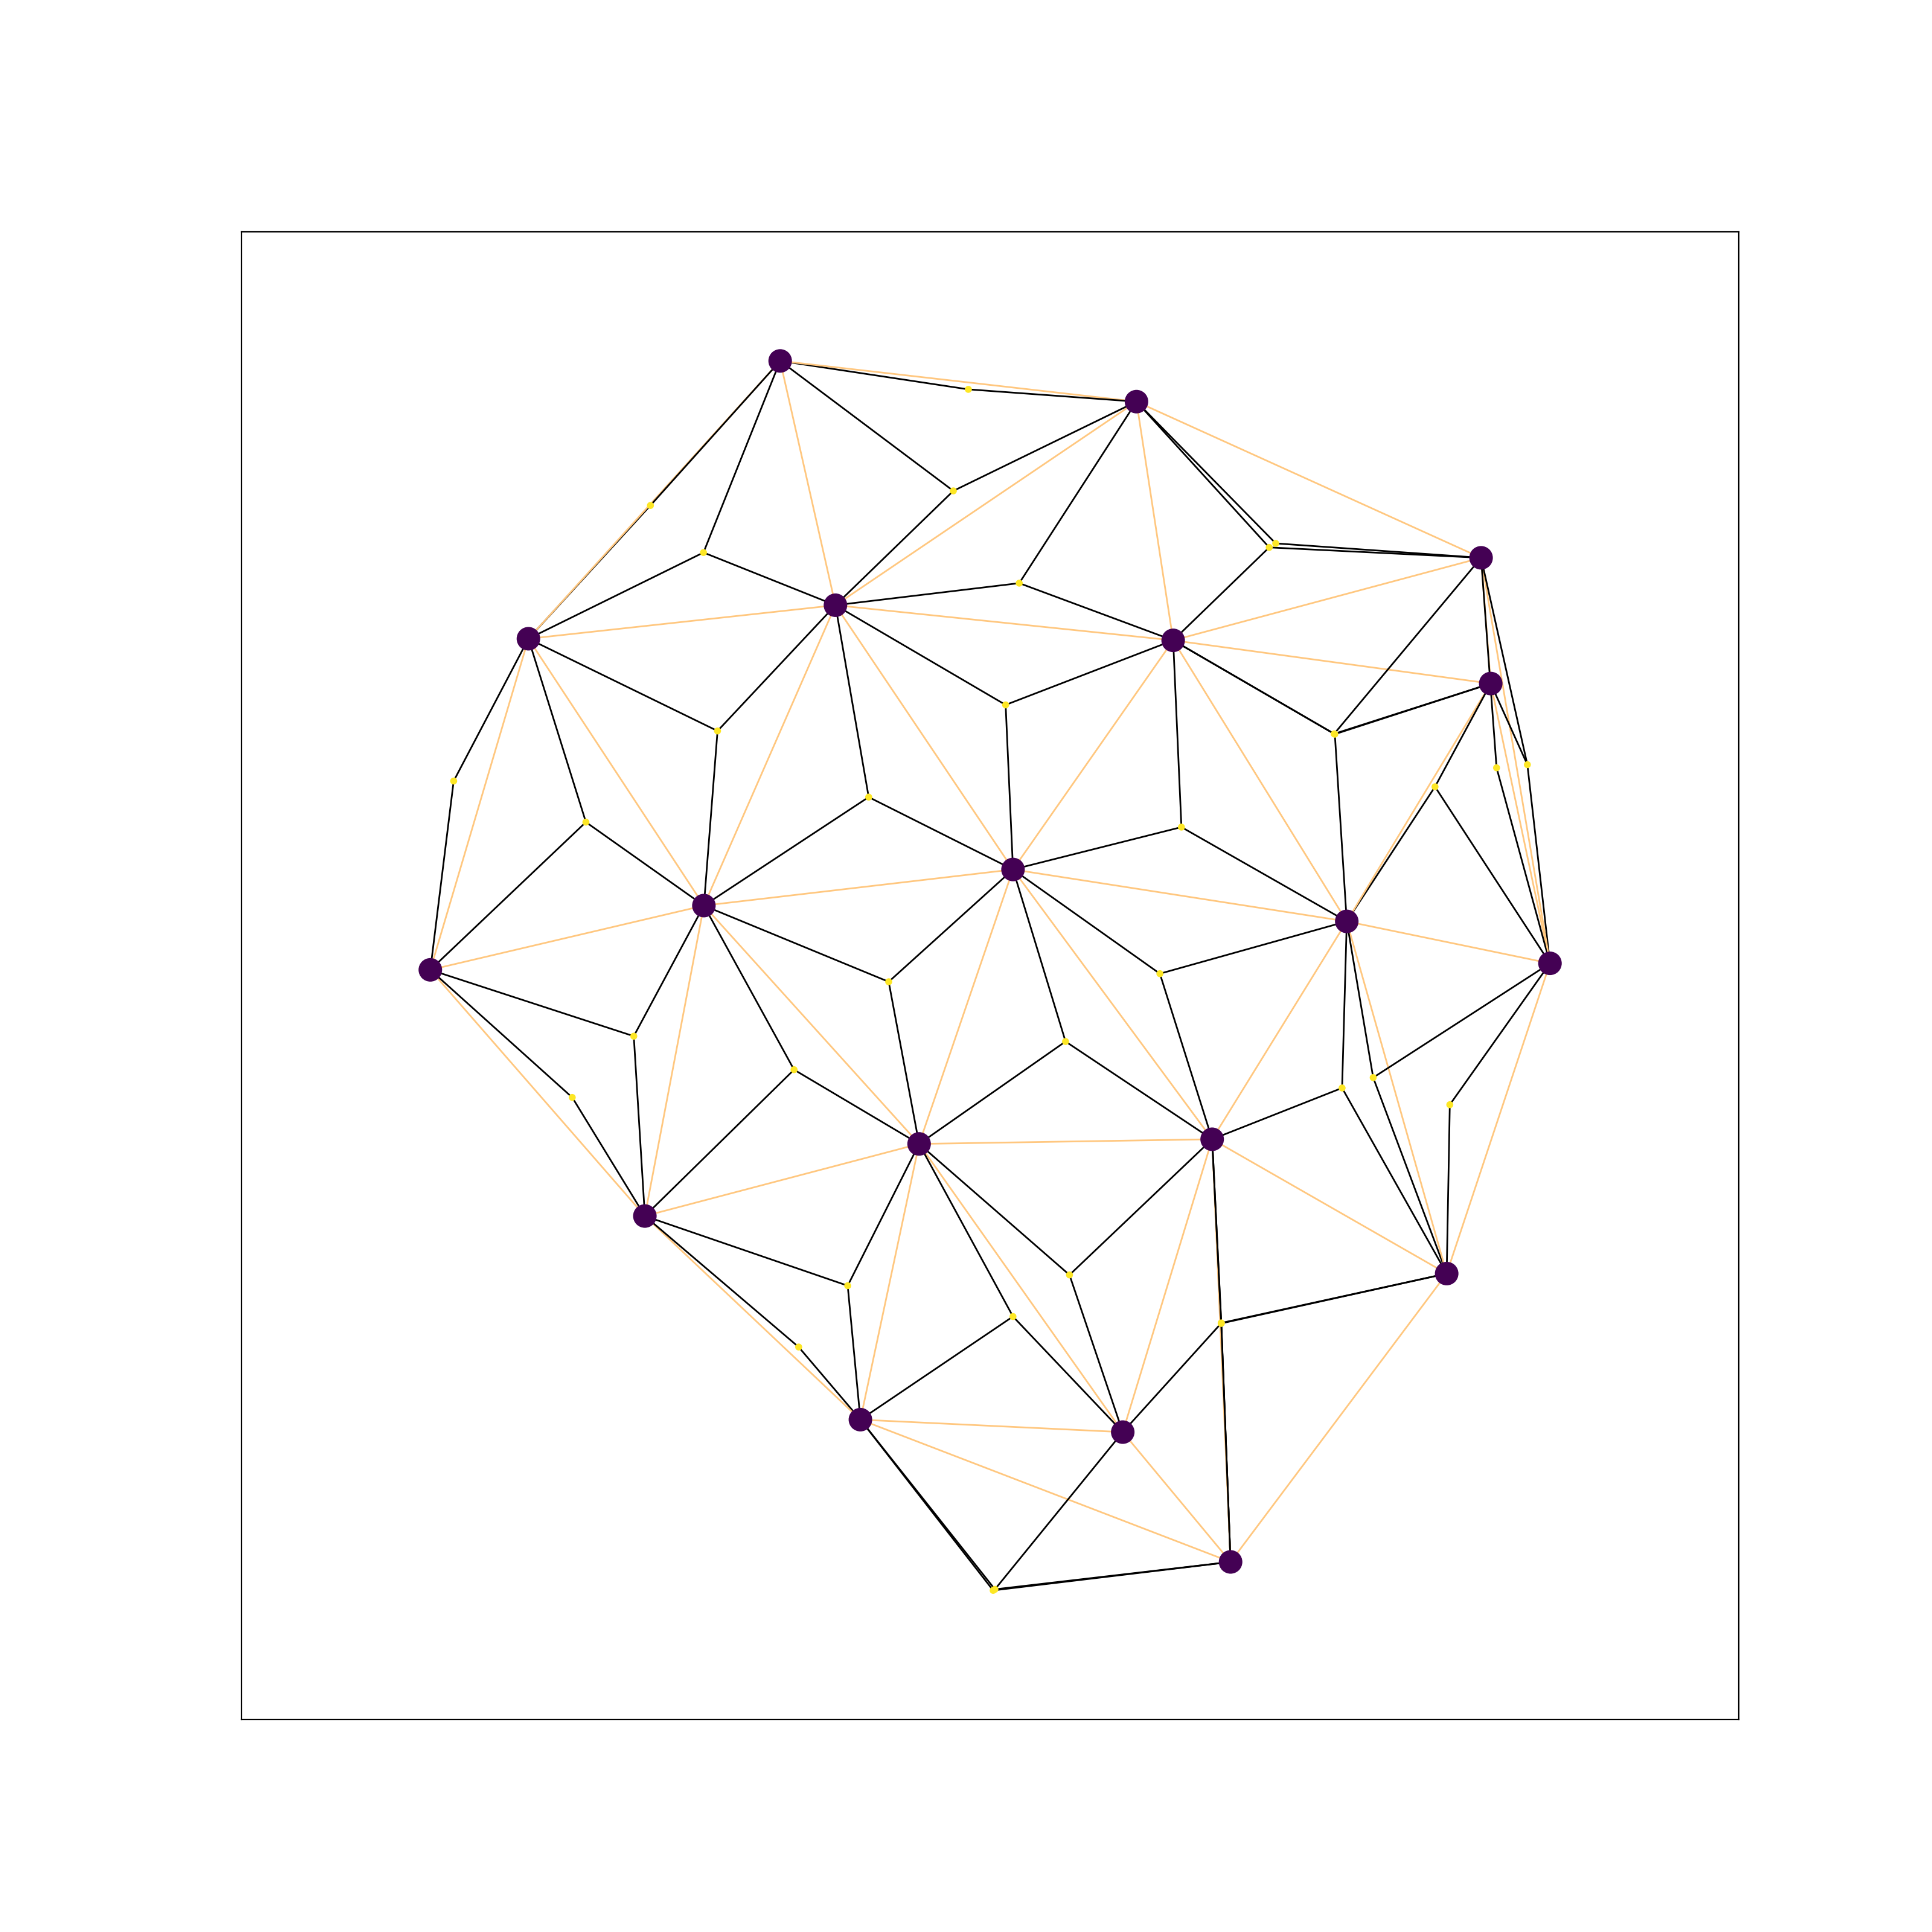
\includegraphics[width=0.3\textwidth]{hexnoise/hexnoise0.8_0.8_1.52_10_graph.png}
        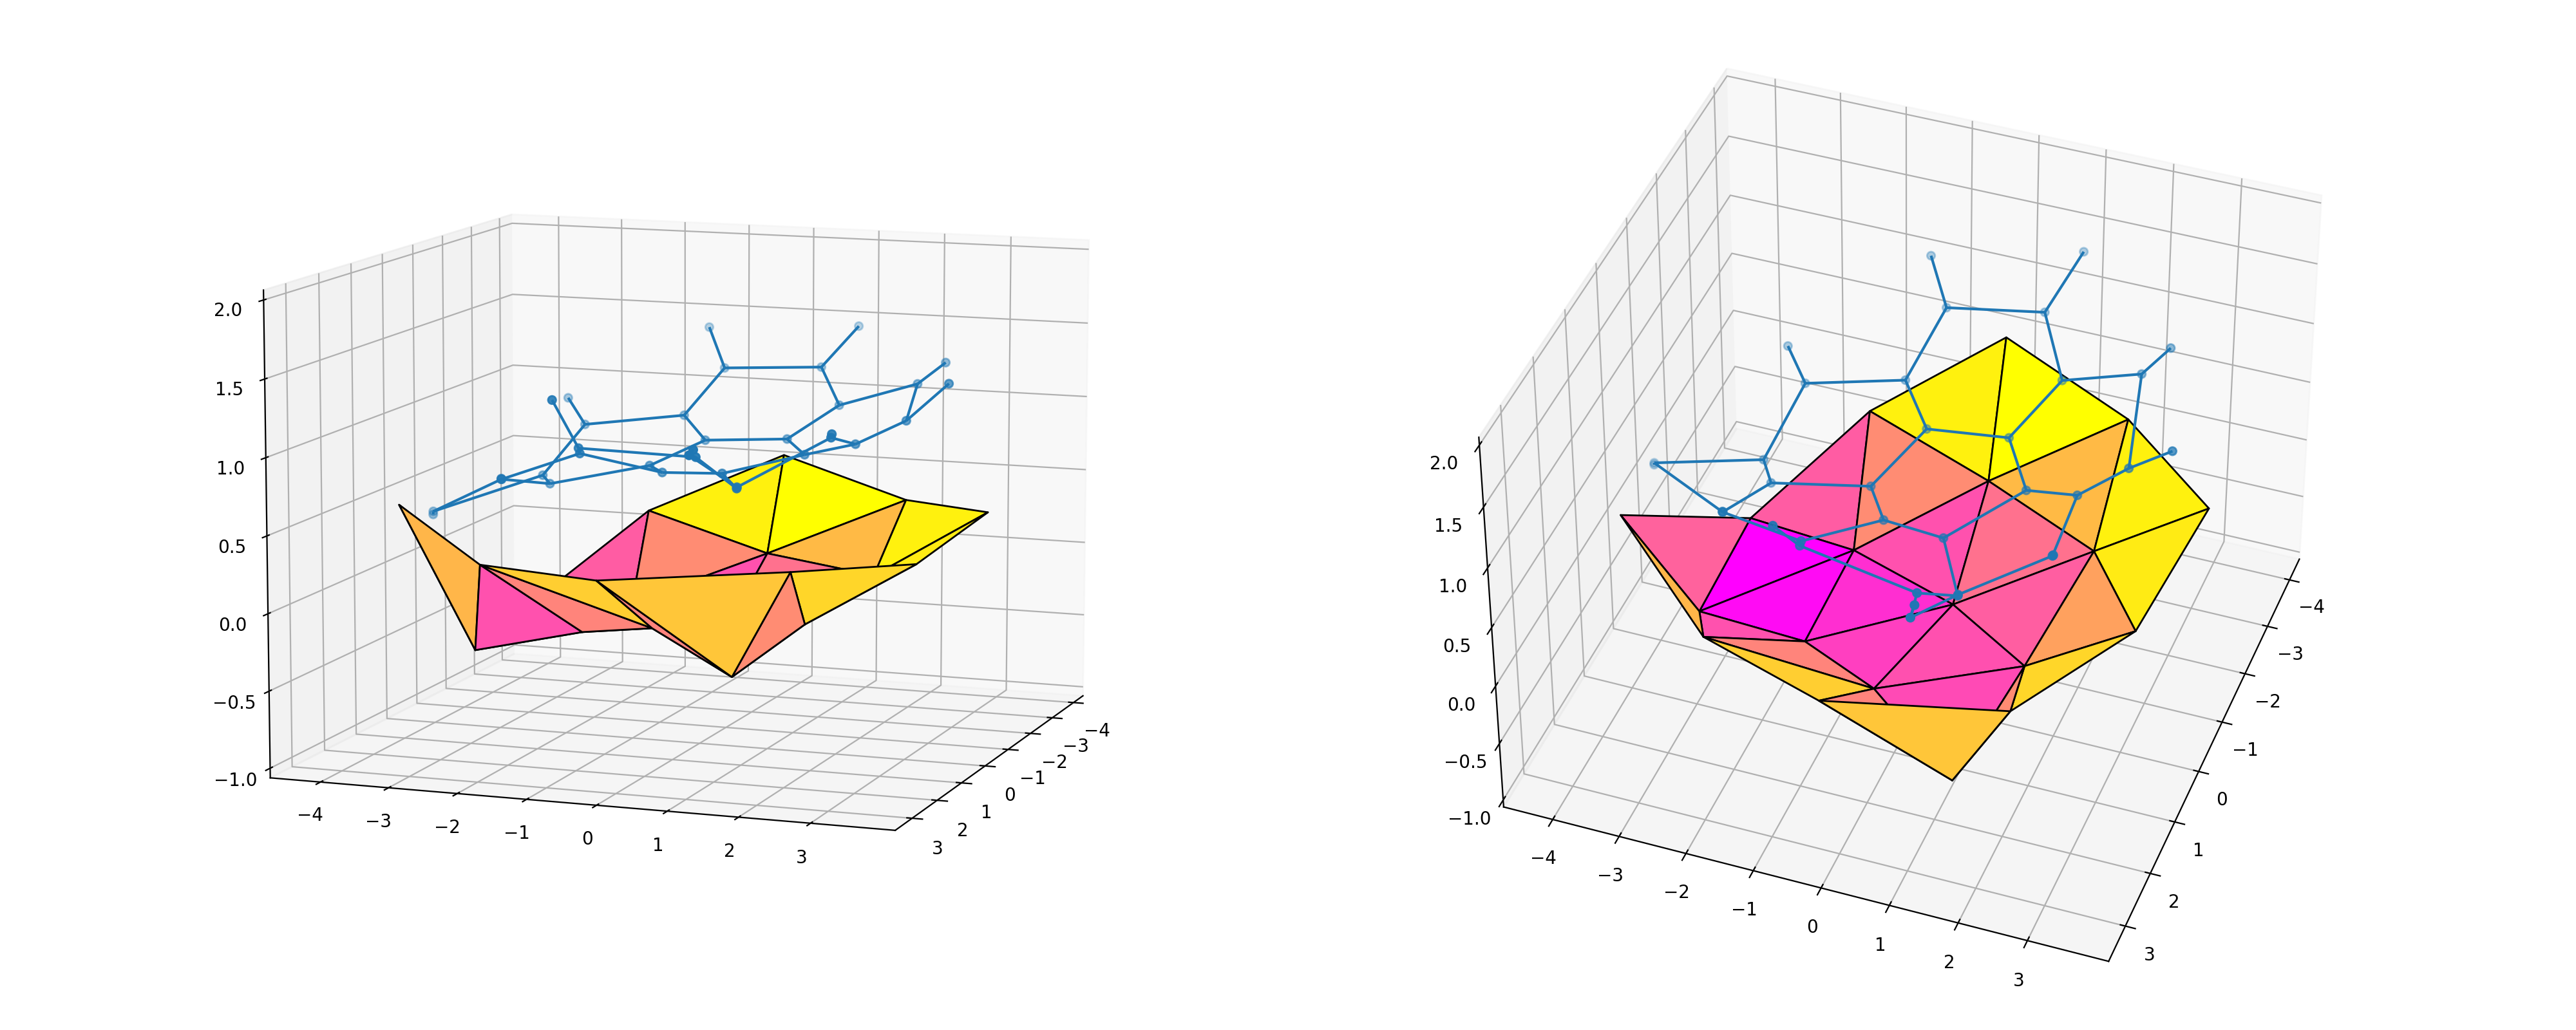
\includegraphics[width=0.69\textwidth]{hexnoise/hexnoise0.8_0.8_1.52_10_plot.png}
        \caption{Sheet shape when $\phi_0=0.8$, $\psi_0=0.8$, $\ell_0=1.52$.}
        \label{subfig:hexnoise_in}
    \end{subfigure}
    \begin{subfigure}[b]{\textwidth}
        \centering
        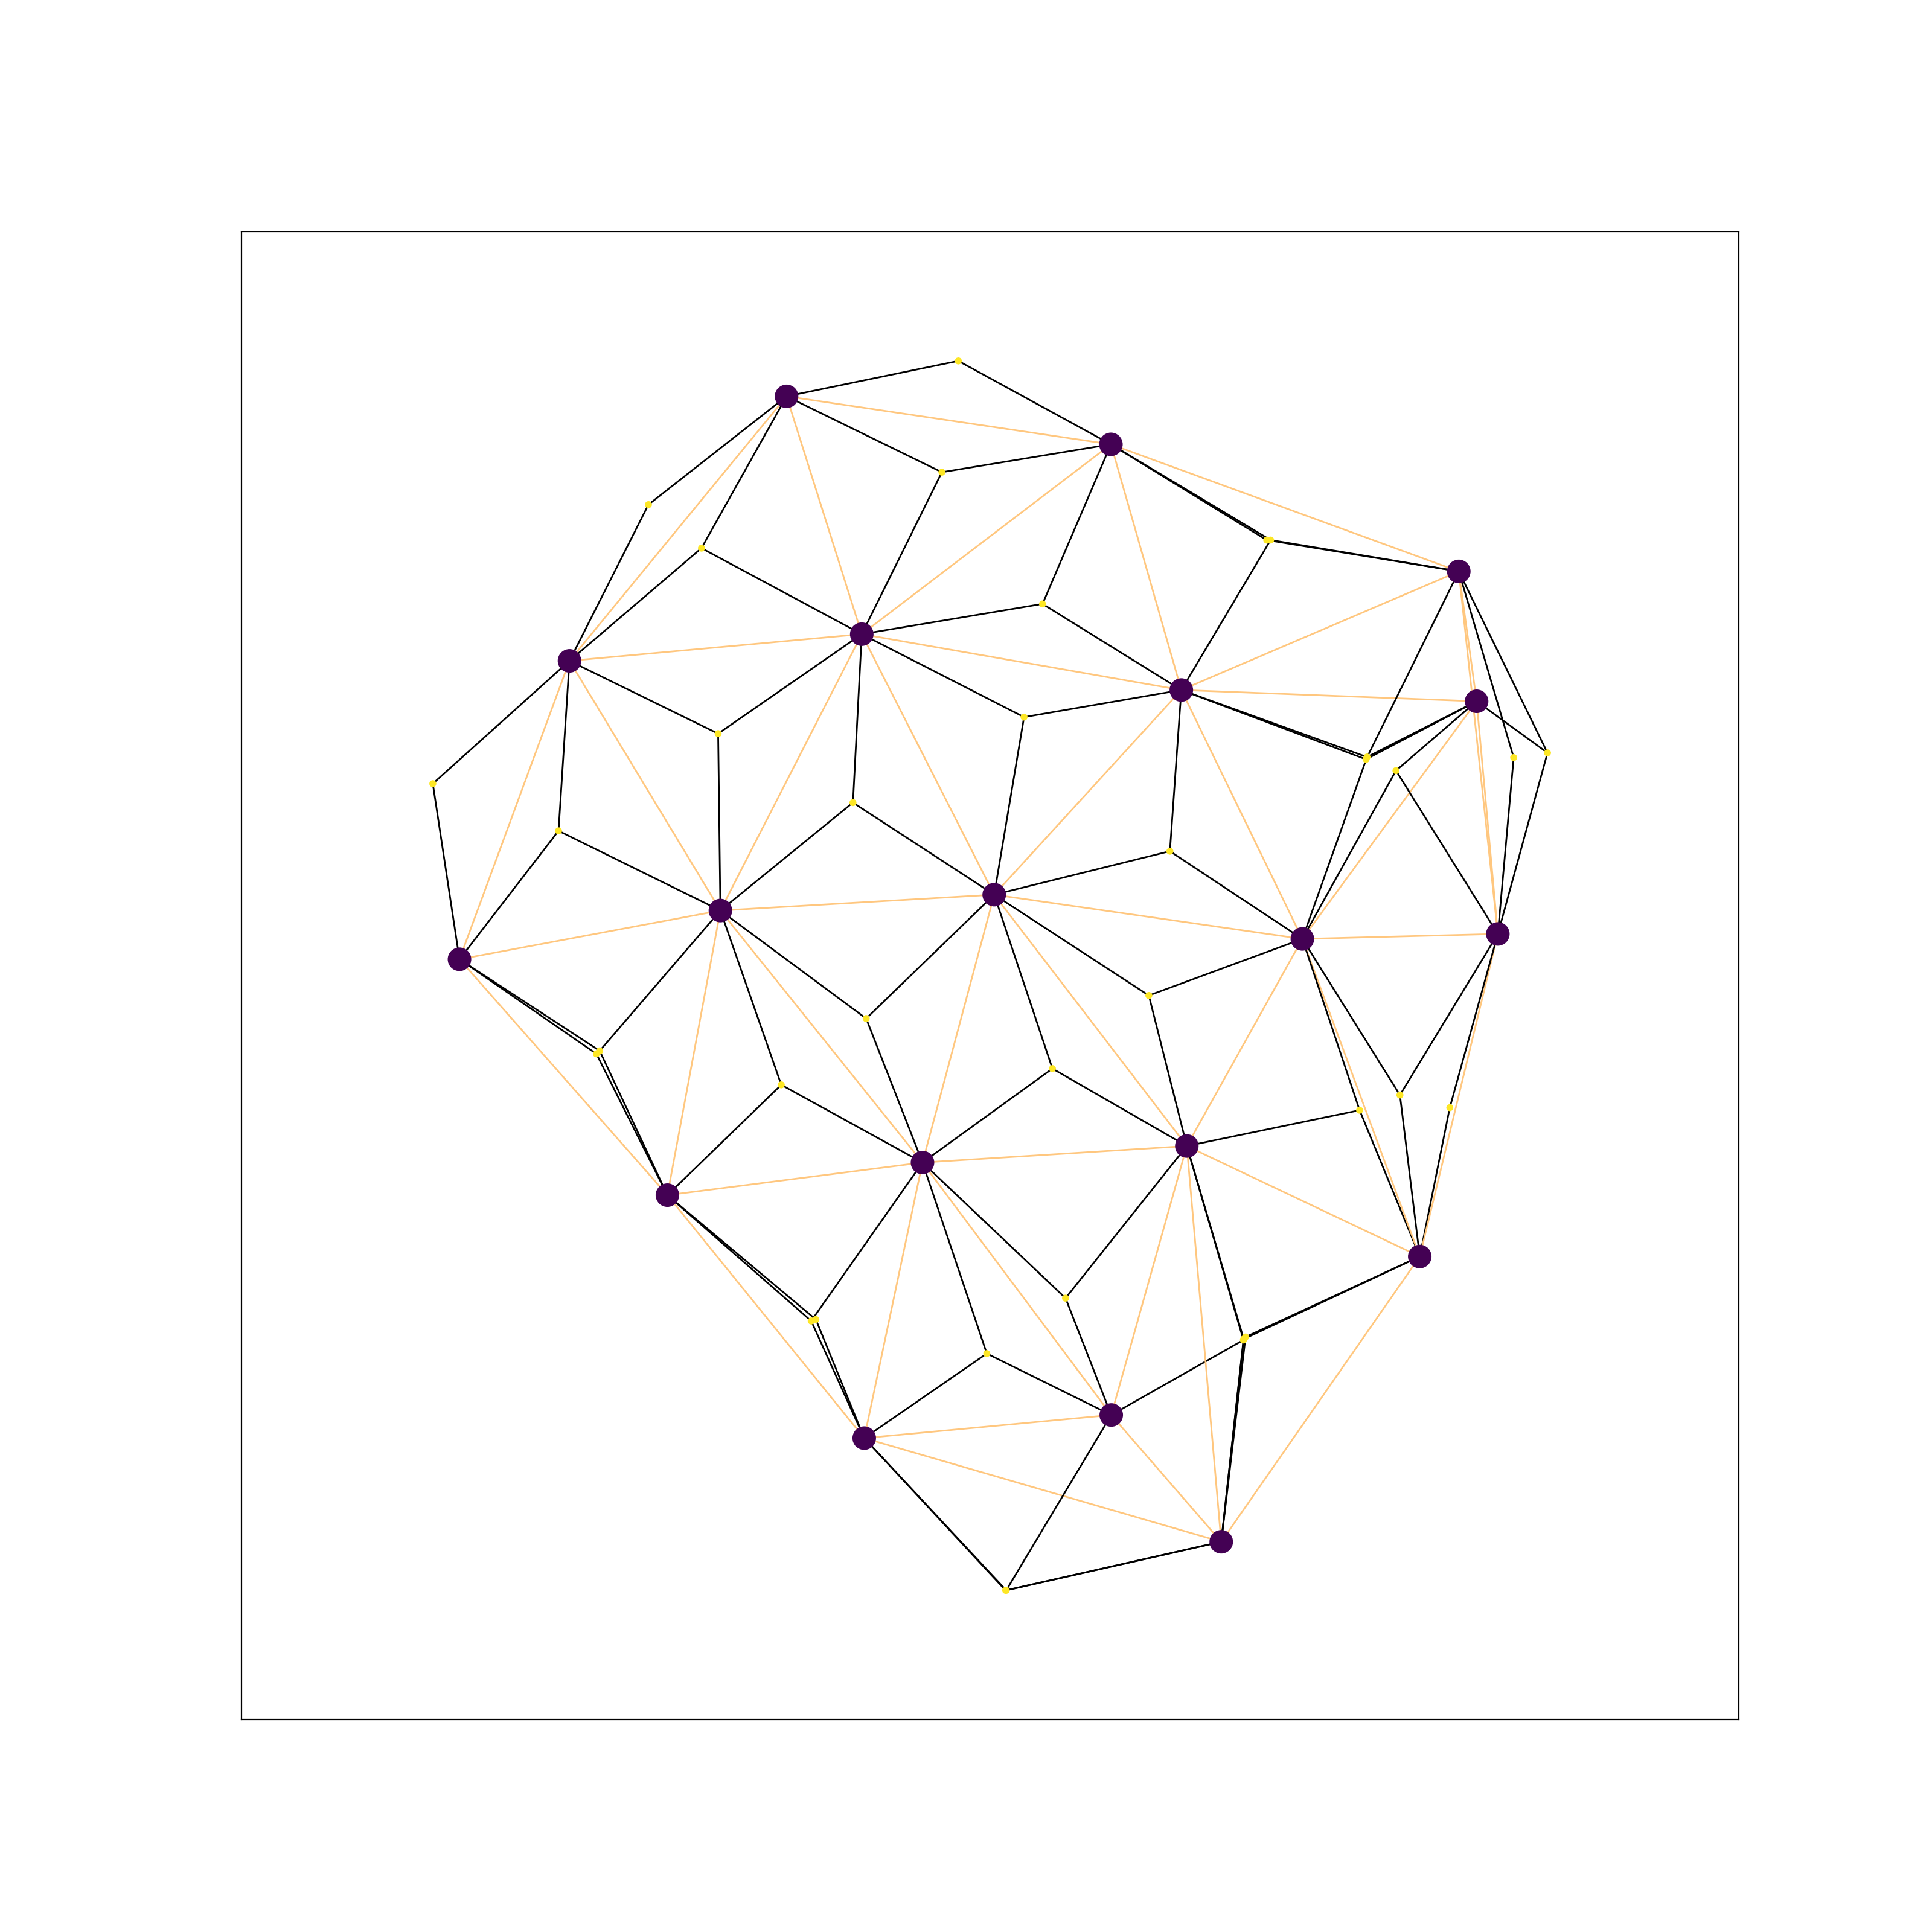
\includegraphics[width=0.3\textwidth]{hexnoise/hexnoise0.95_0.8_1.52_10_graph.png}
        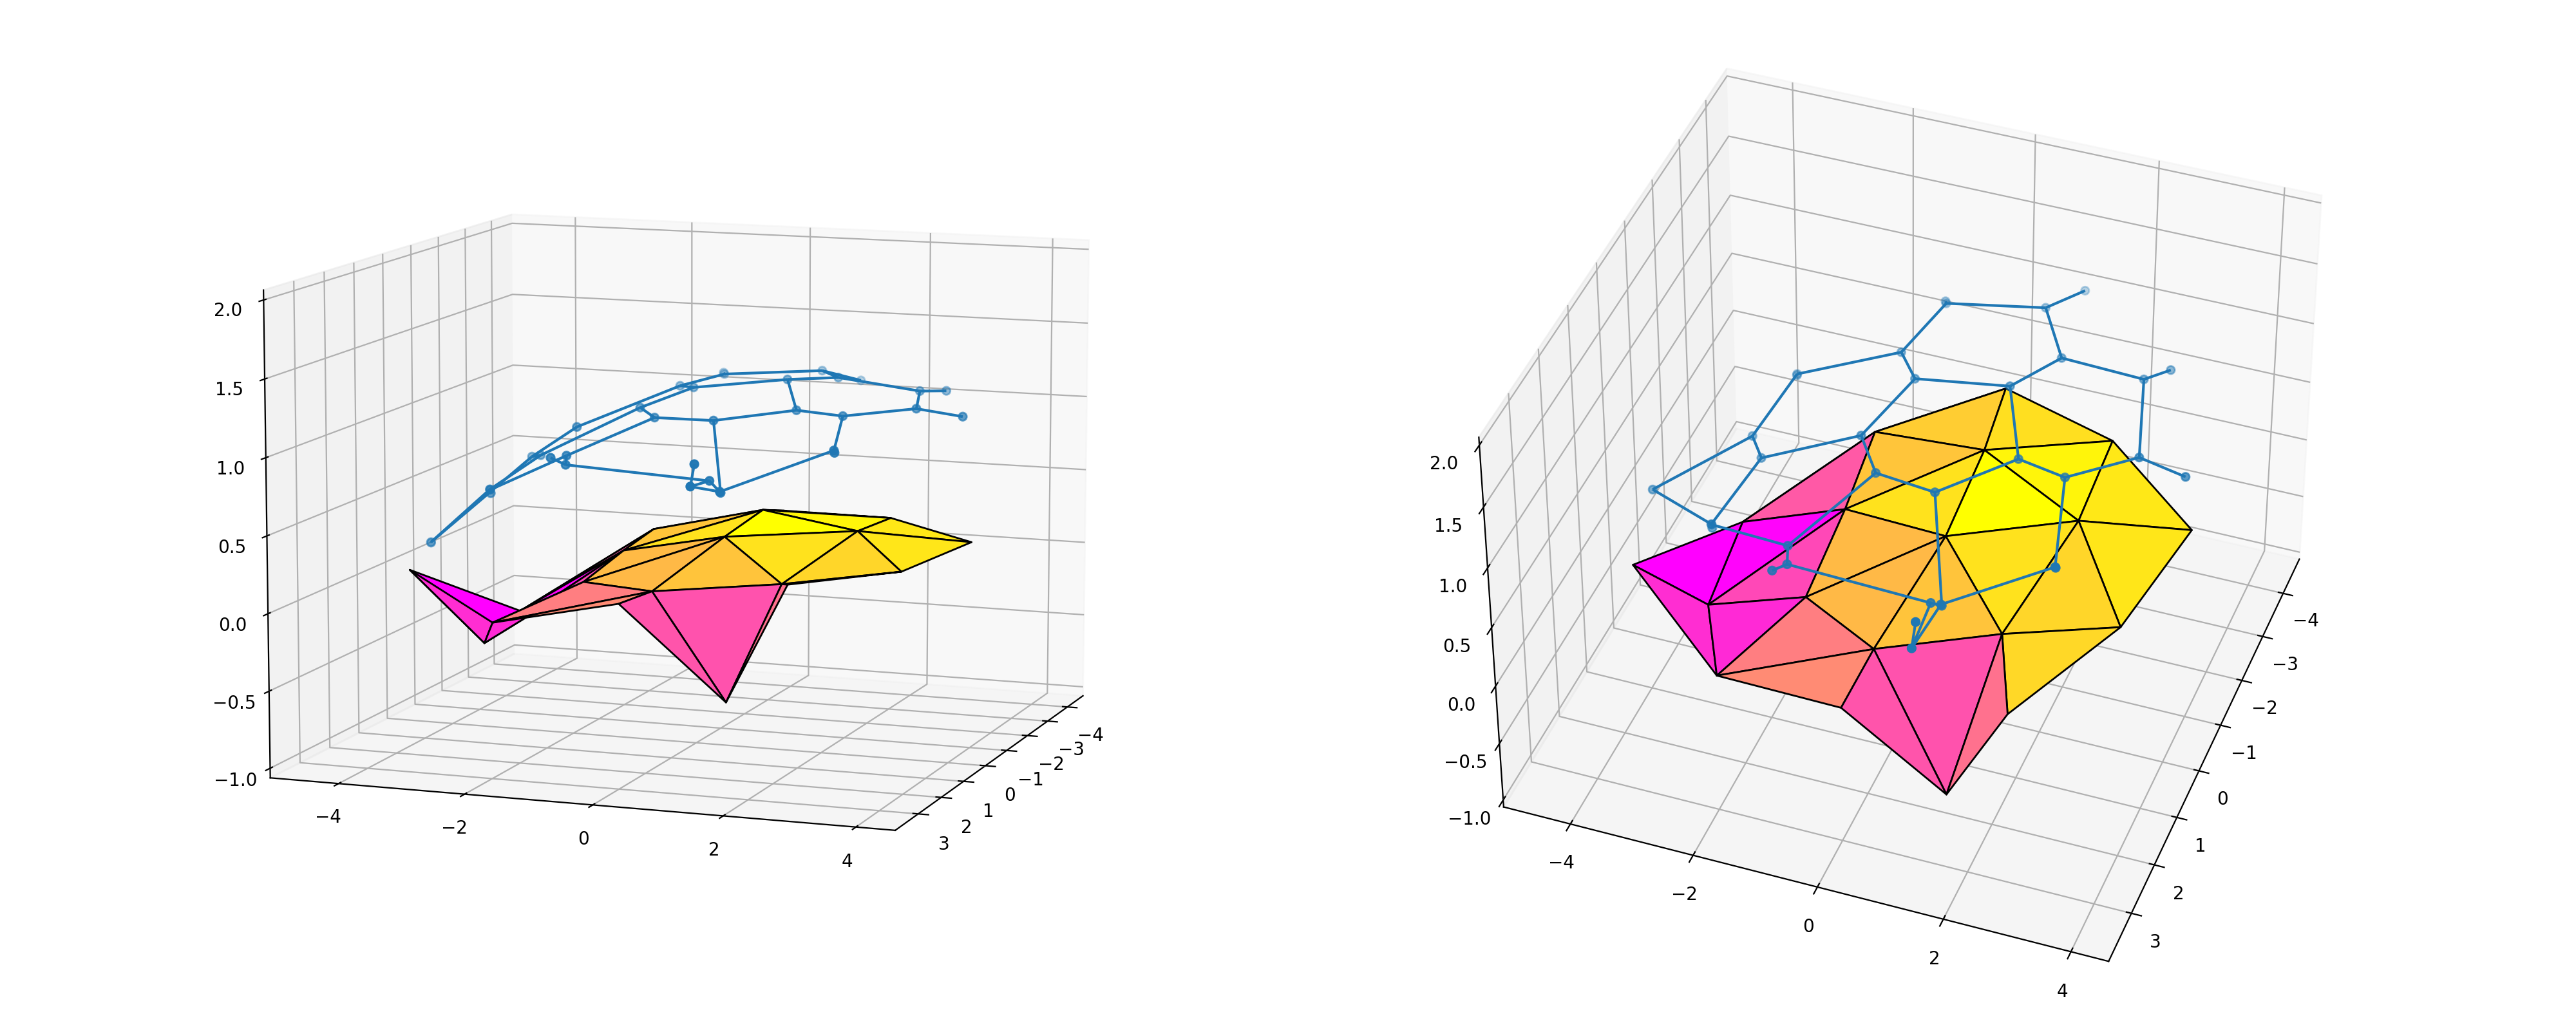
\includegraphics[width=0.69\textwidth]{hexnoise/hexnoise0.95_0.8_1.52_10_plot.png}
        \caption{Sheet shape when $\phi_0=0.95$, $\psi_0=0.8$, $\ell_0=1.52$.}
        \label{subfig:hexnoise_out}
    \end{subfigure}
    \caption{Cell sheet geometry with noise added to the initial lattice. The graph topology is affected at the sheet boundary (subfigure \ref{subfig:hexnoise_graph}) from the Voronoi tesselation. This minor change has substantial effects on the sheet geometry (subfigures \ref{subfig:hexnoise_in}, \ref{subfig:hexnoise_out}).}
    \label{fig:hexnoise}
\end{figure}

\subsubsection{Interior cell topology}

We can also add or merge nodes in a regular lattice (Figure \ref{fig:layout_init}) to introduce nodes with irregular degree. There are more complex ways of making different graph topologies (like Lloyd's initial icosphere) but I don't have curved initial conditions or more complicated lattices implemented yet. 

Figure \ref{fig:kink} shows a sheet with cell of degree 7 (7 bordering cells) and \ref{fig:bump} shows a sheet with two neighboring cells of degree 5. 

\begin{figure}[htbp]
    \centering
    \begin{subfigure}[b]{\textwidth}
        \centering
        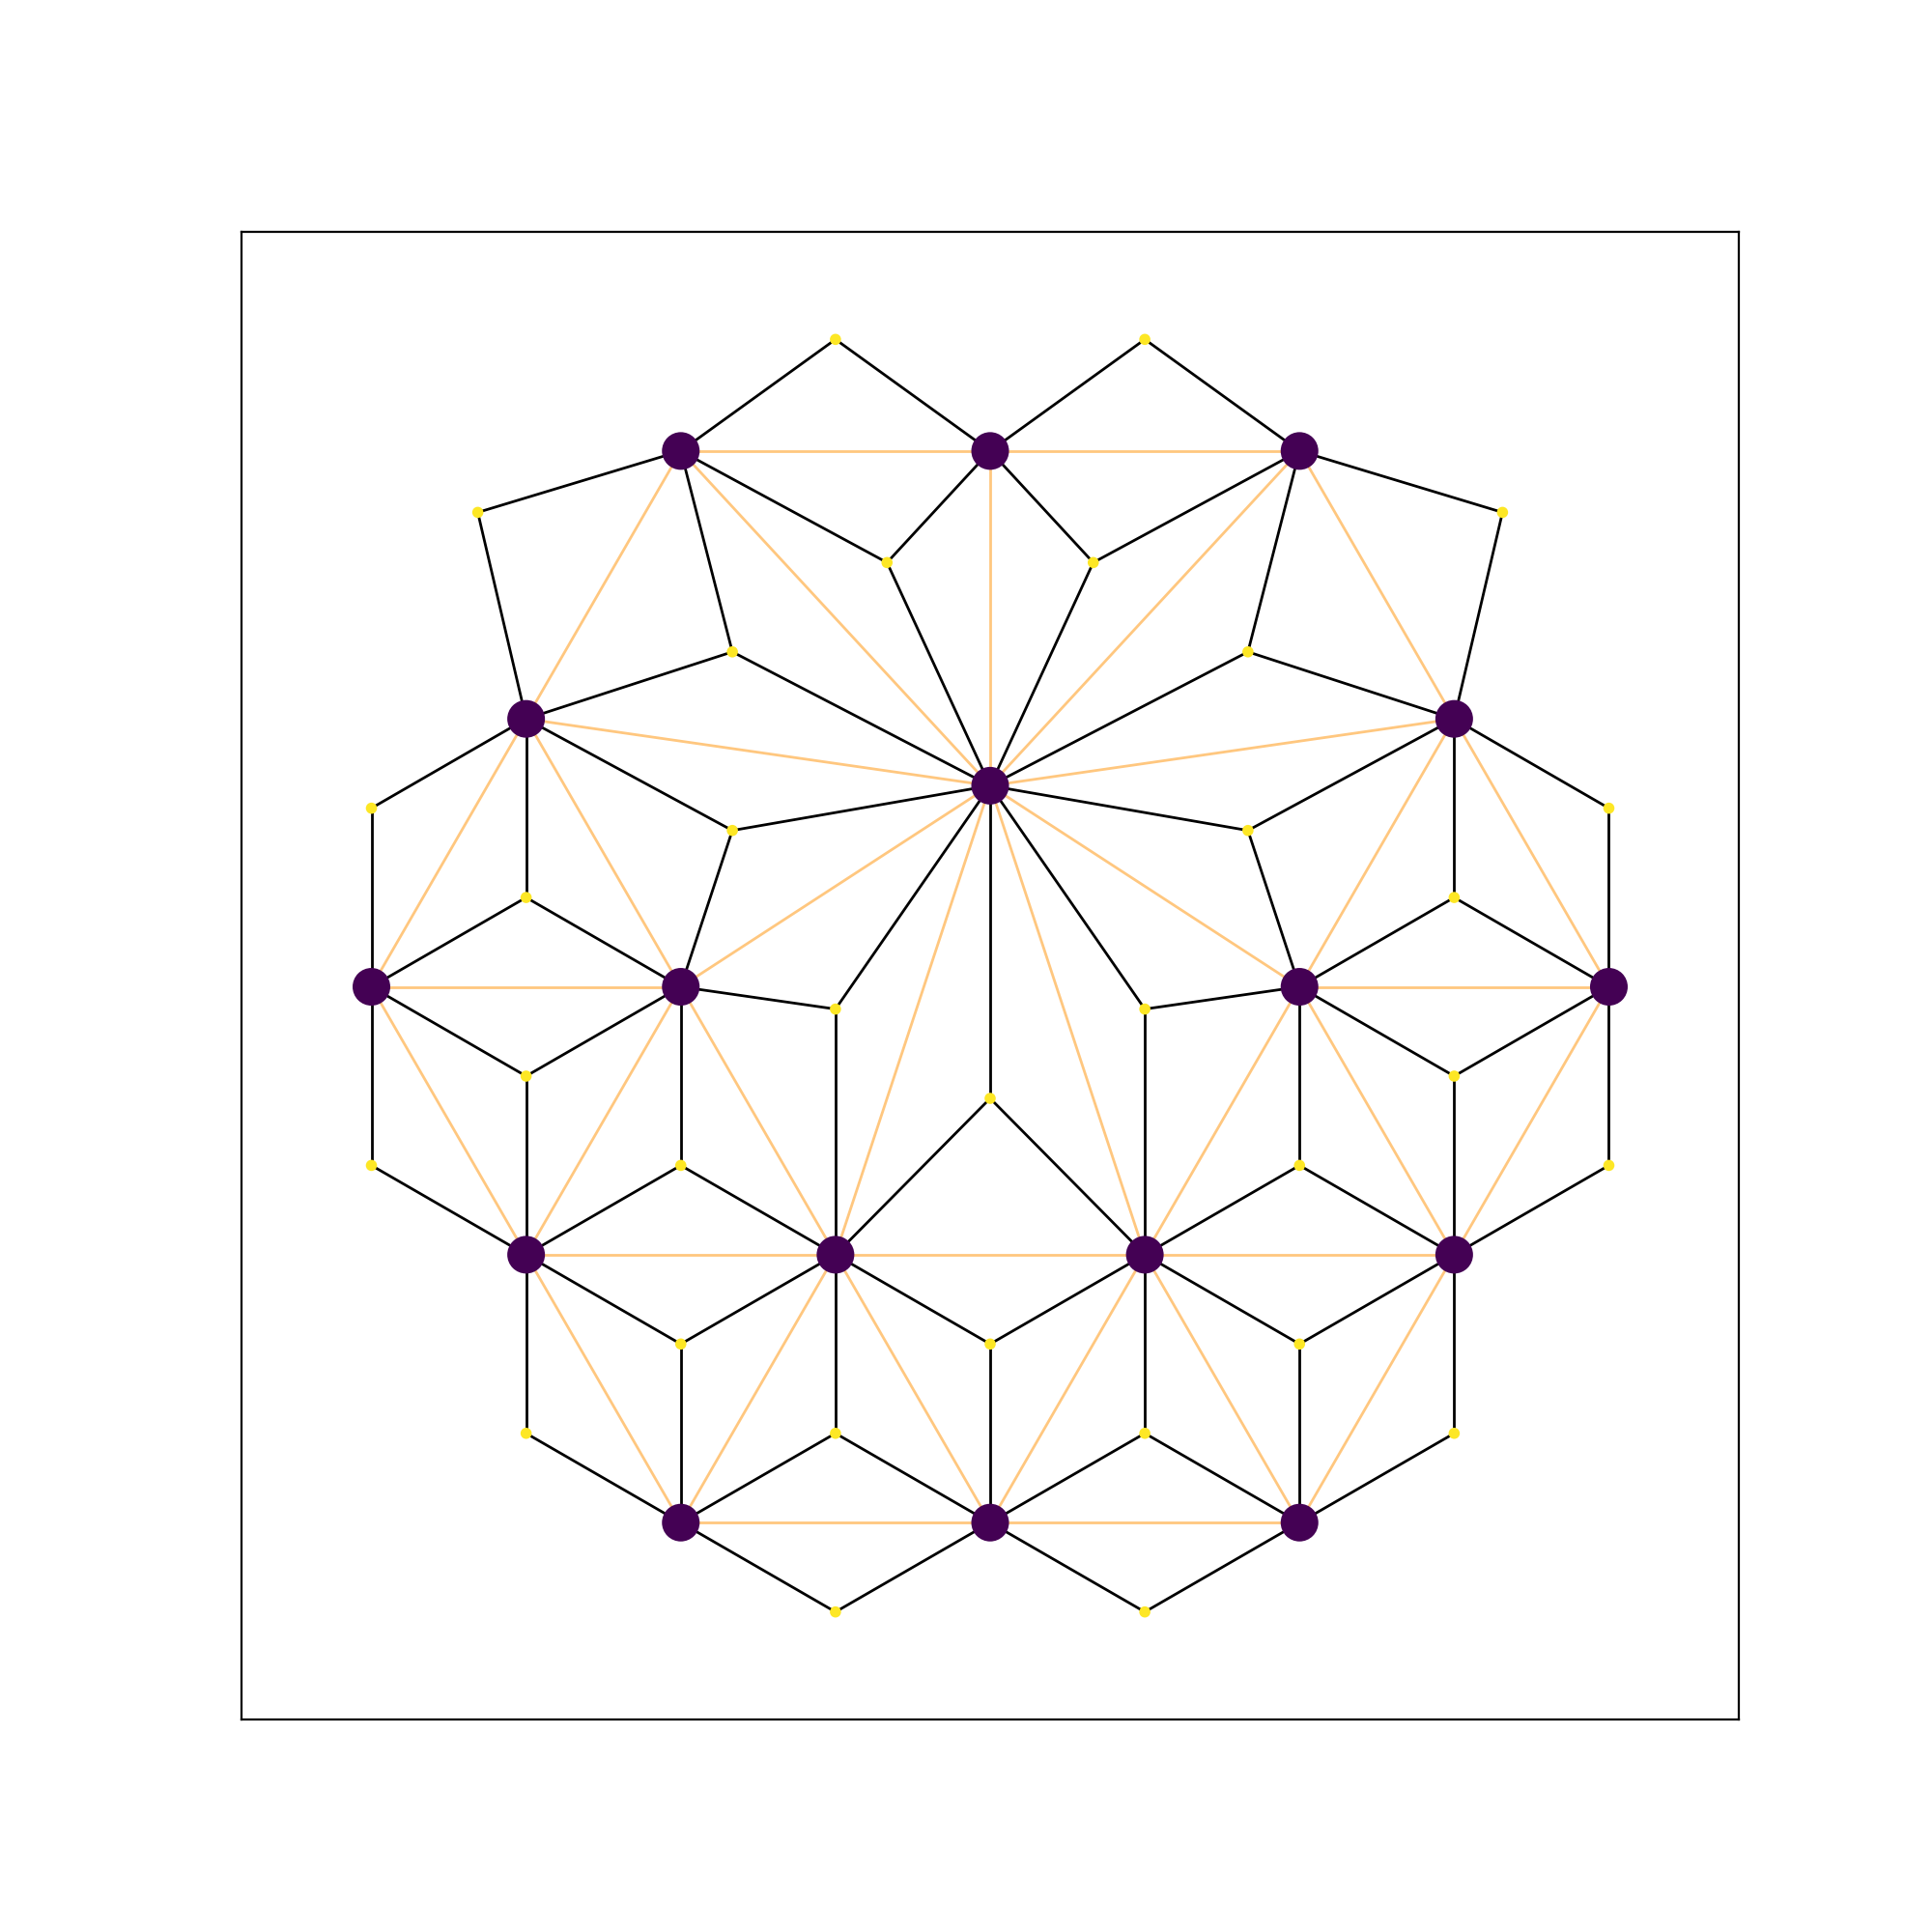
\includegraphics[width=0.5\textwidth]{kink/kink_graph.png}
        \caption{Initial lattice drawn as in Figure \ref{fig:layout_init}.}
        \label{subfig:kink_graph}
    \end{subfigure}
    \begin{subfigure}[b]{\textwidth}
        \centering
        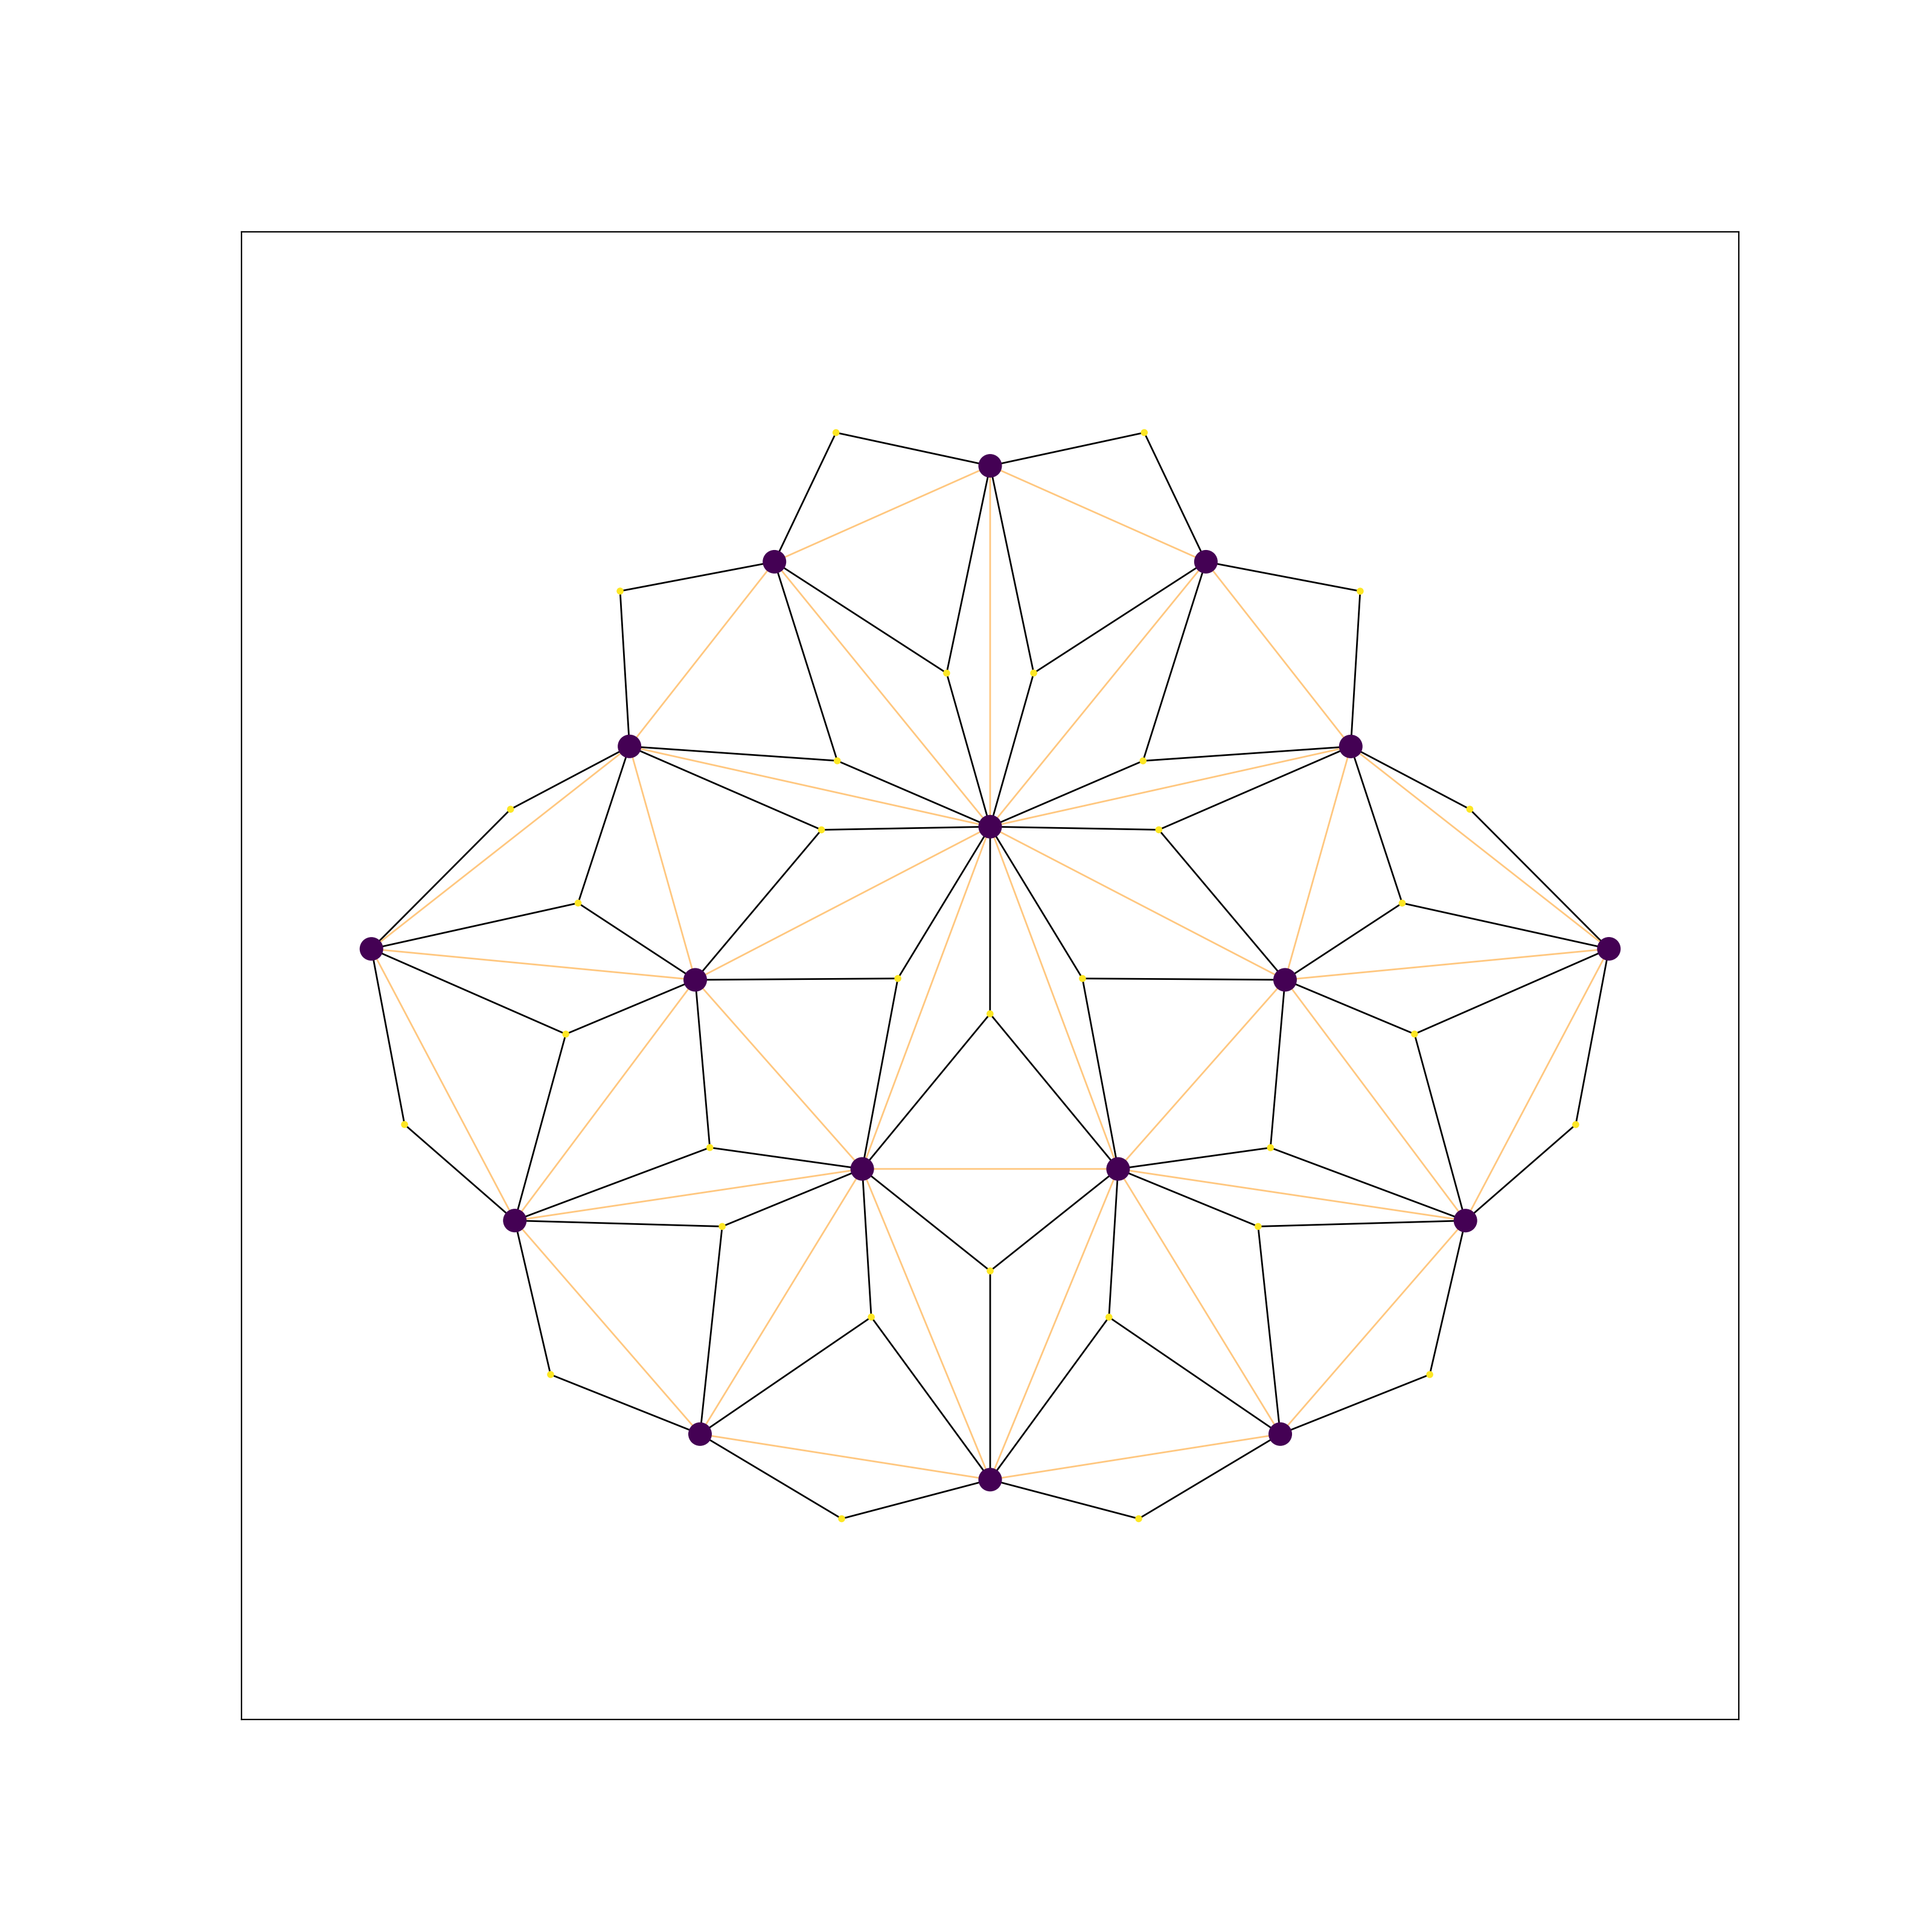
\includegraphics[width=0.3\textwidth]{kink/kink0.8_0.8_1.52_10_graph.png}
        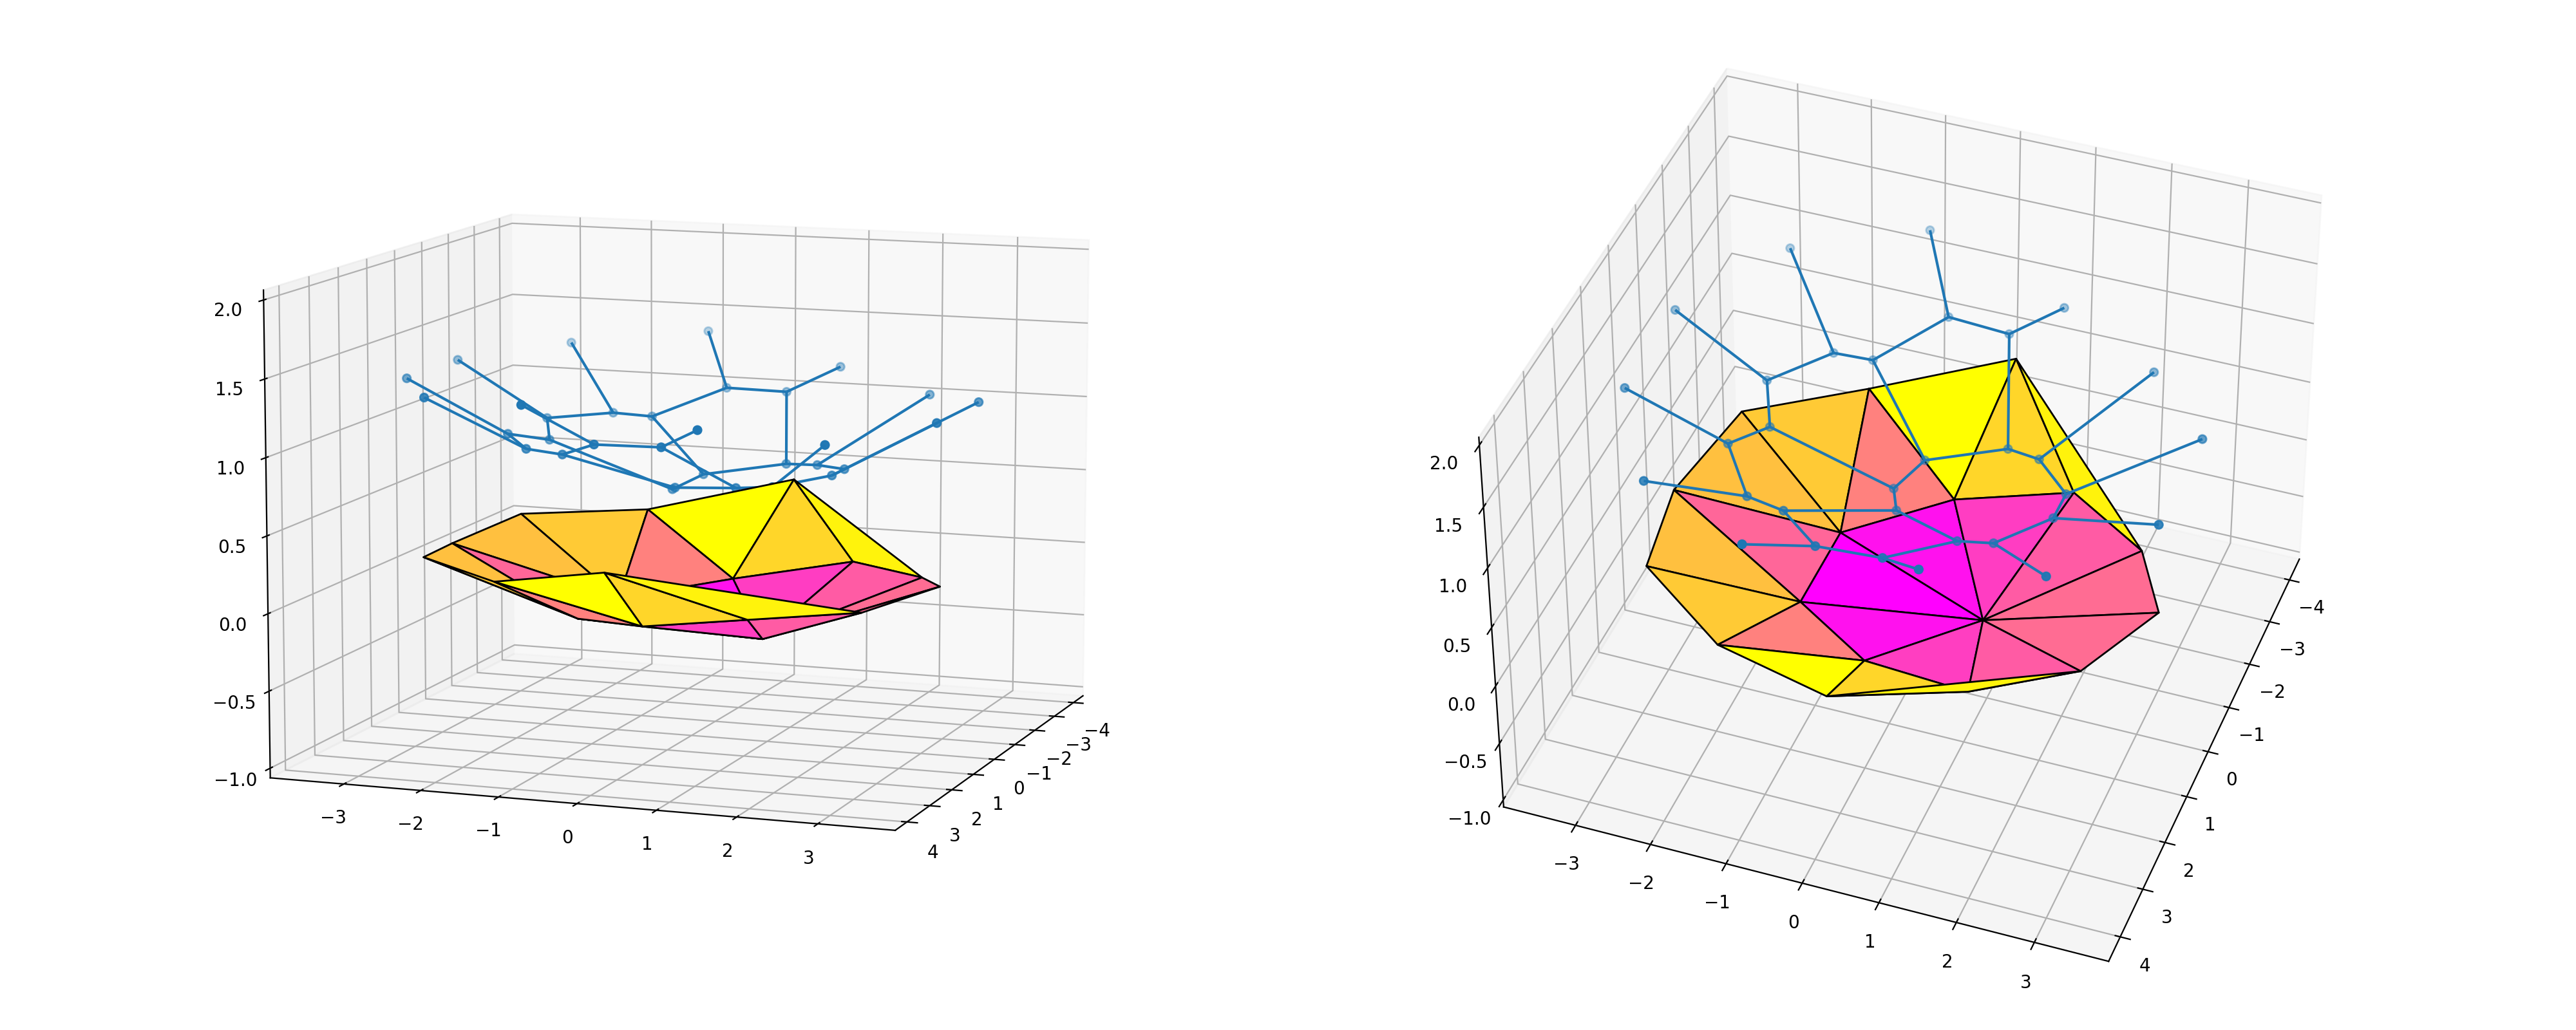
\includegraphics[width=0.69\textwidth]{kink/kink0.8_0.8_1.52_10_plot.png}
        \caption{Sheet shape when $\phi_0=0.8$, $\psi_0=0.8$, $\ell_0=1.52$.}
        \label{subfig:kink_in}
    \end{subfigure}
    \begin{subfigure}[b]{\textwidth}
        \centering
        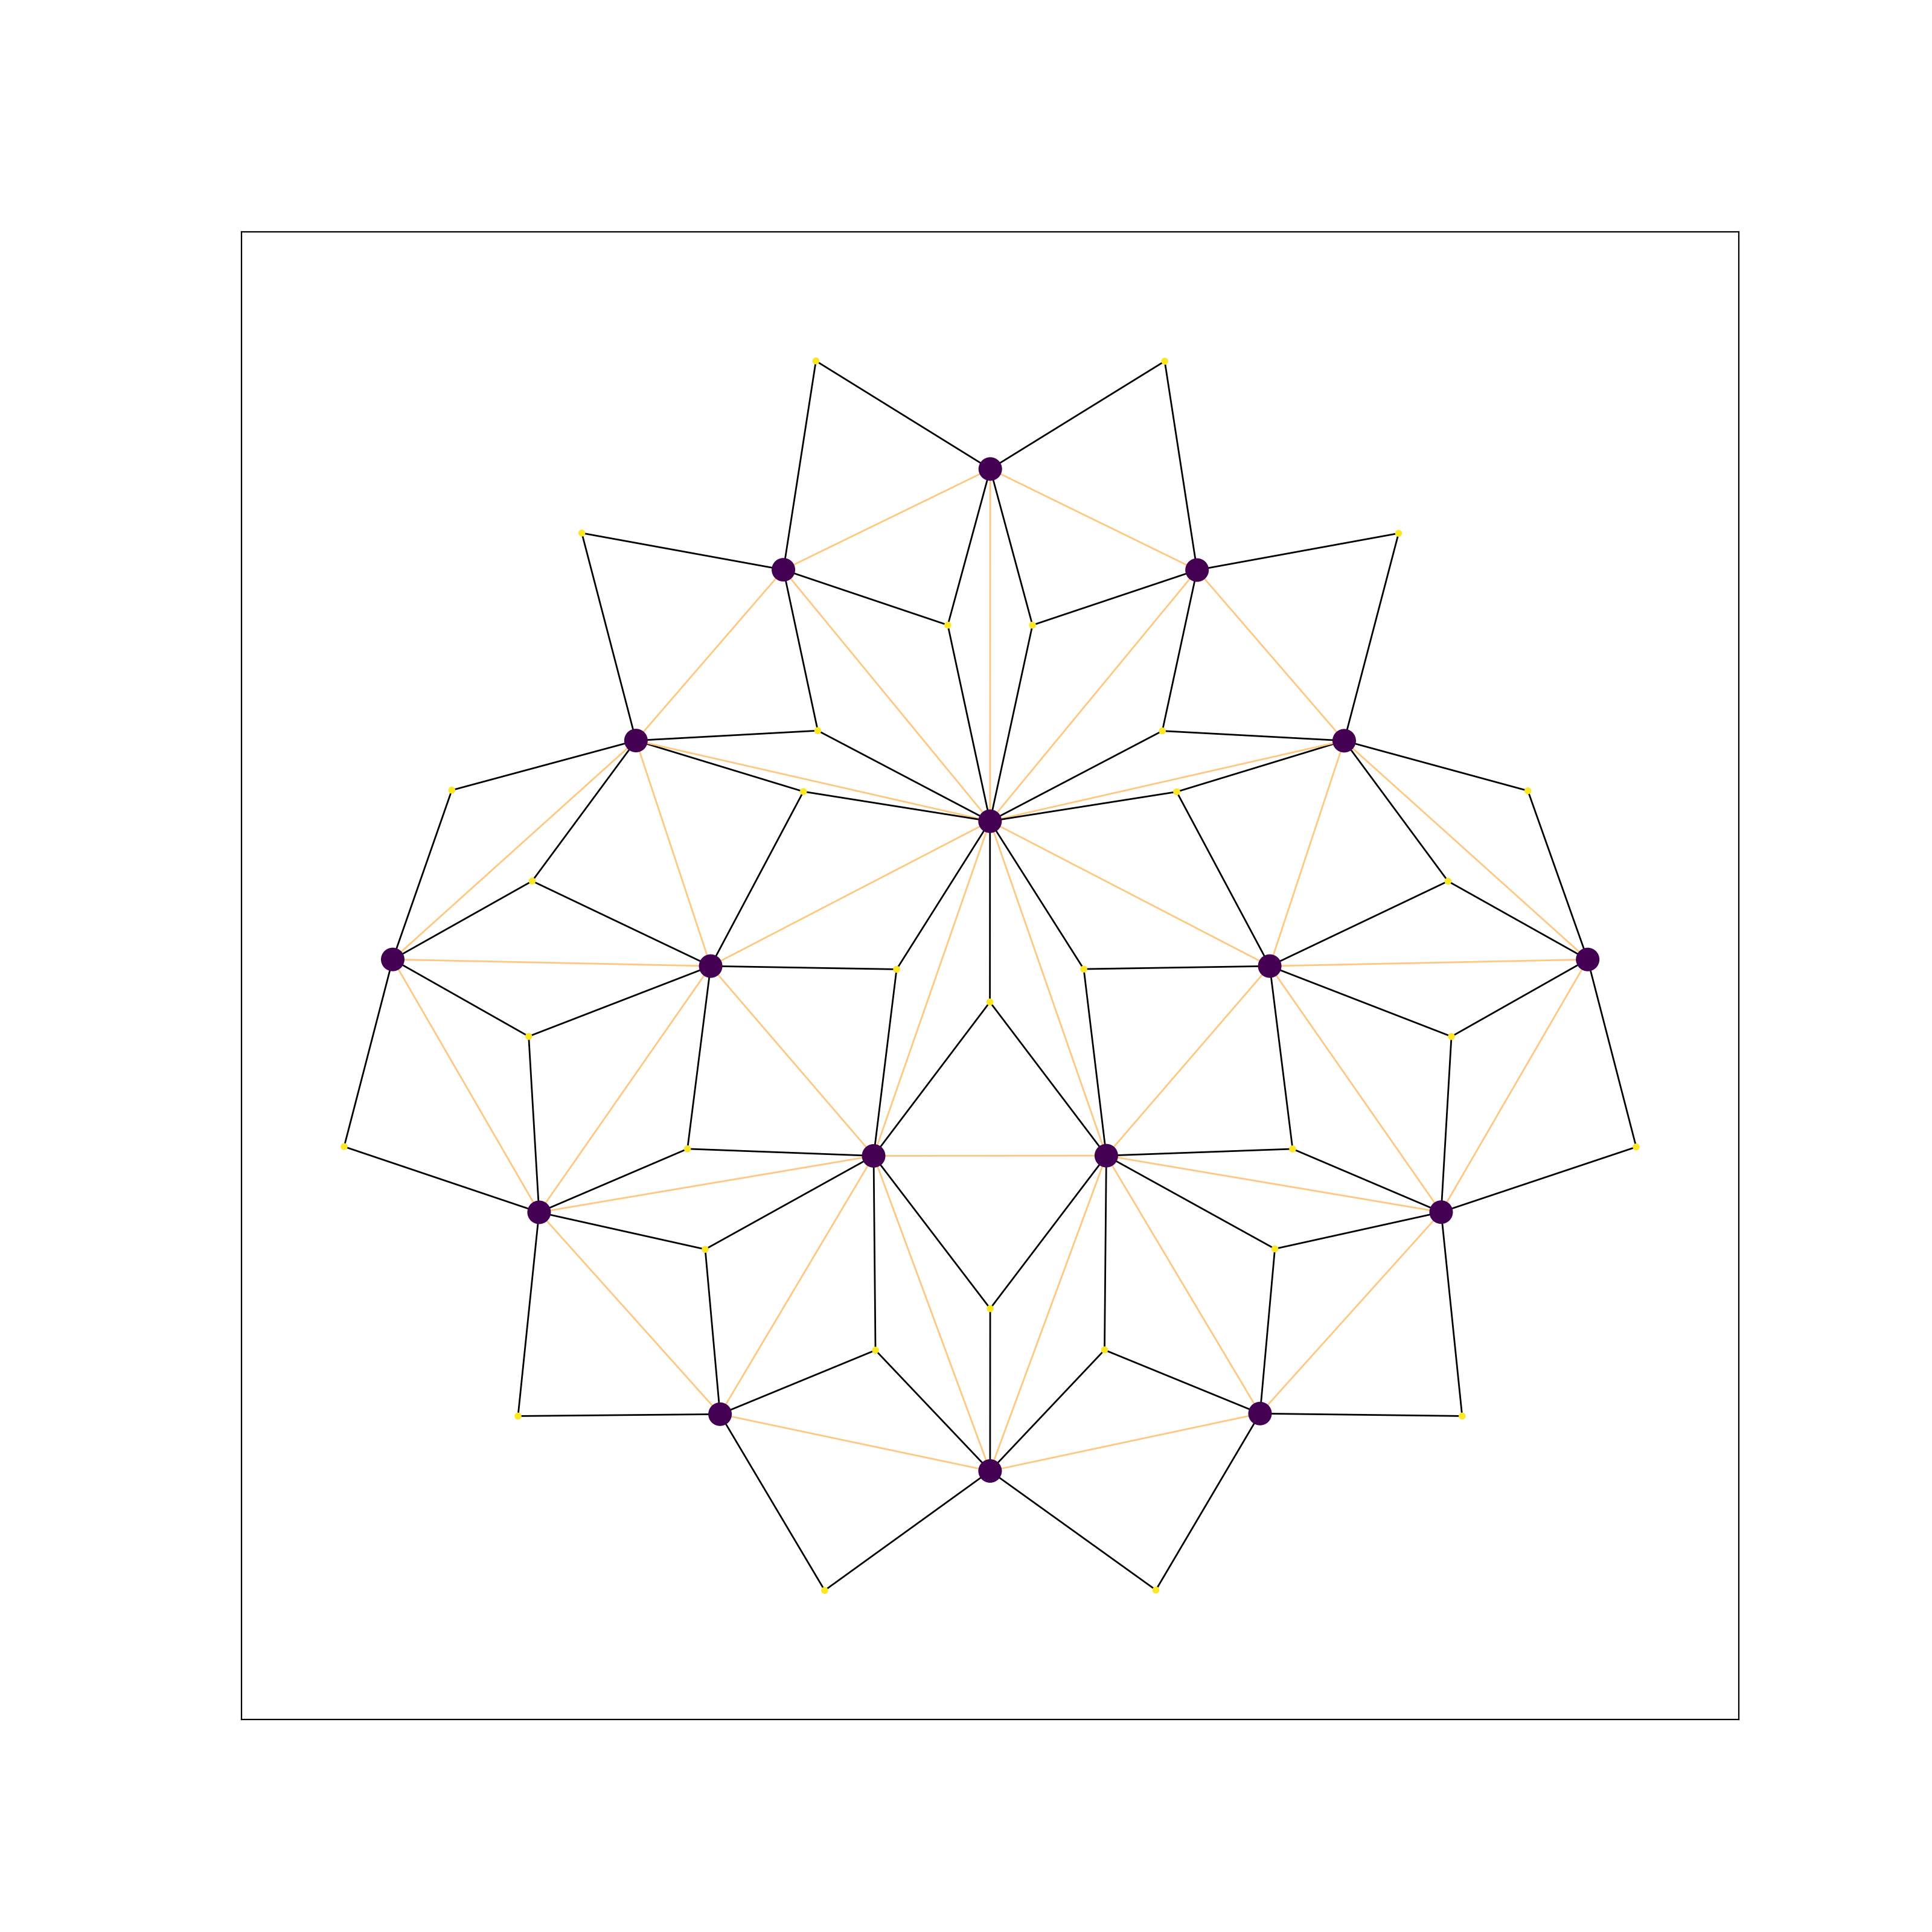
\includegraphics[width=0.3\textwidth]{kink/kink0.95_0.8_1.52_10_graph.png}
        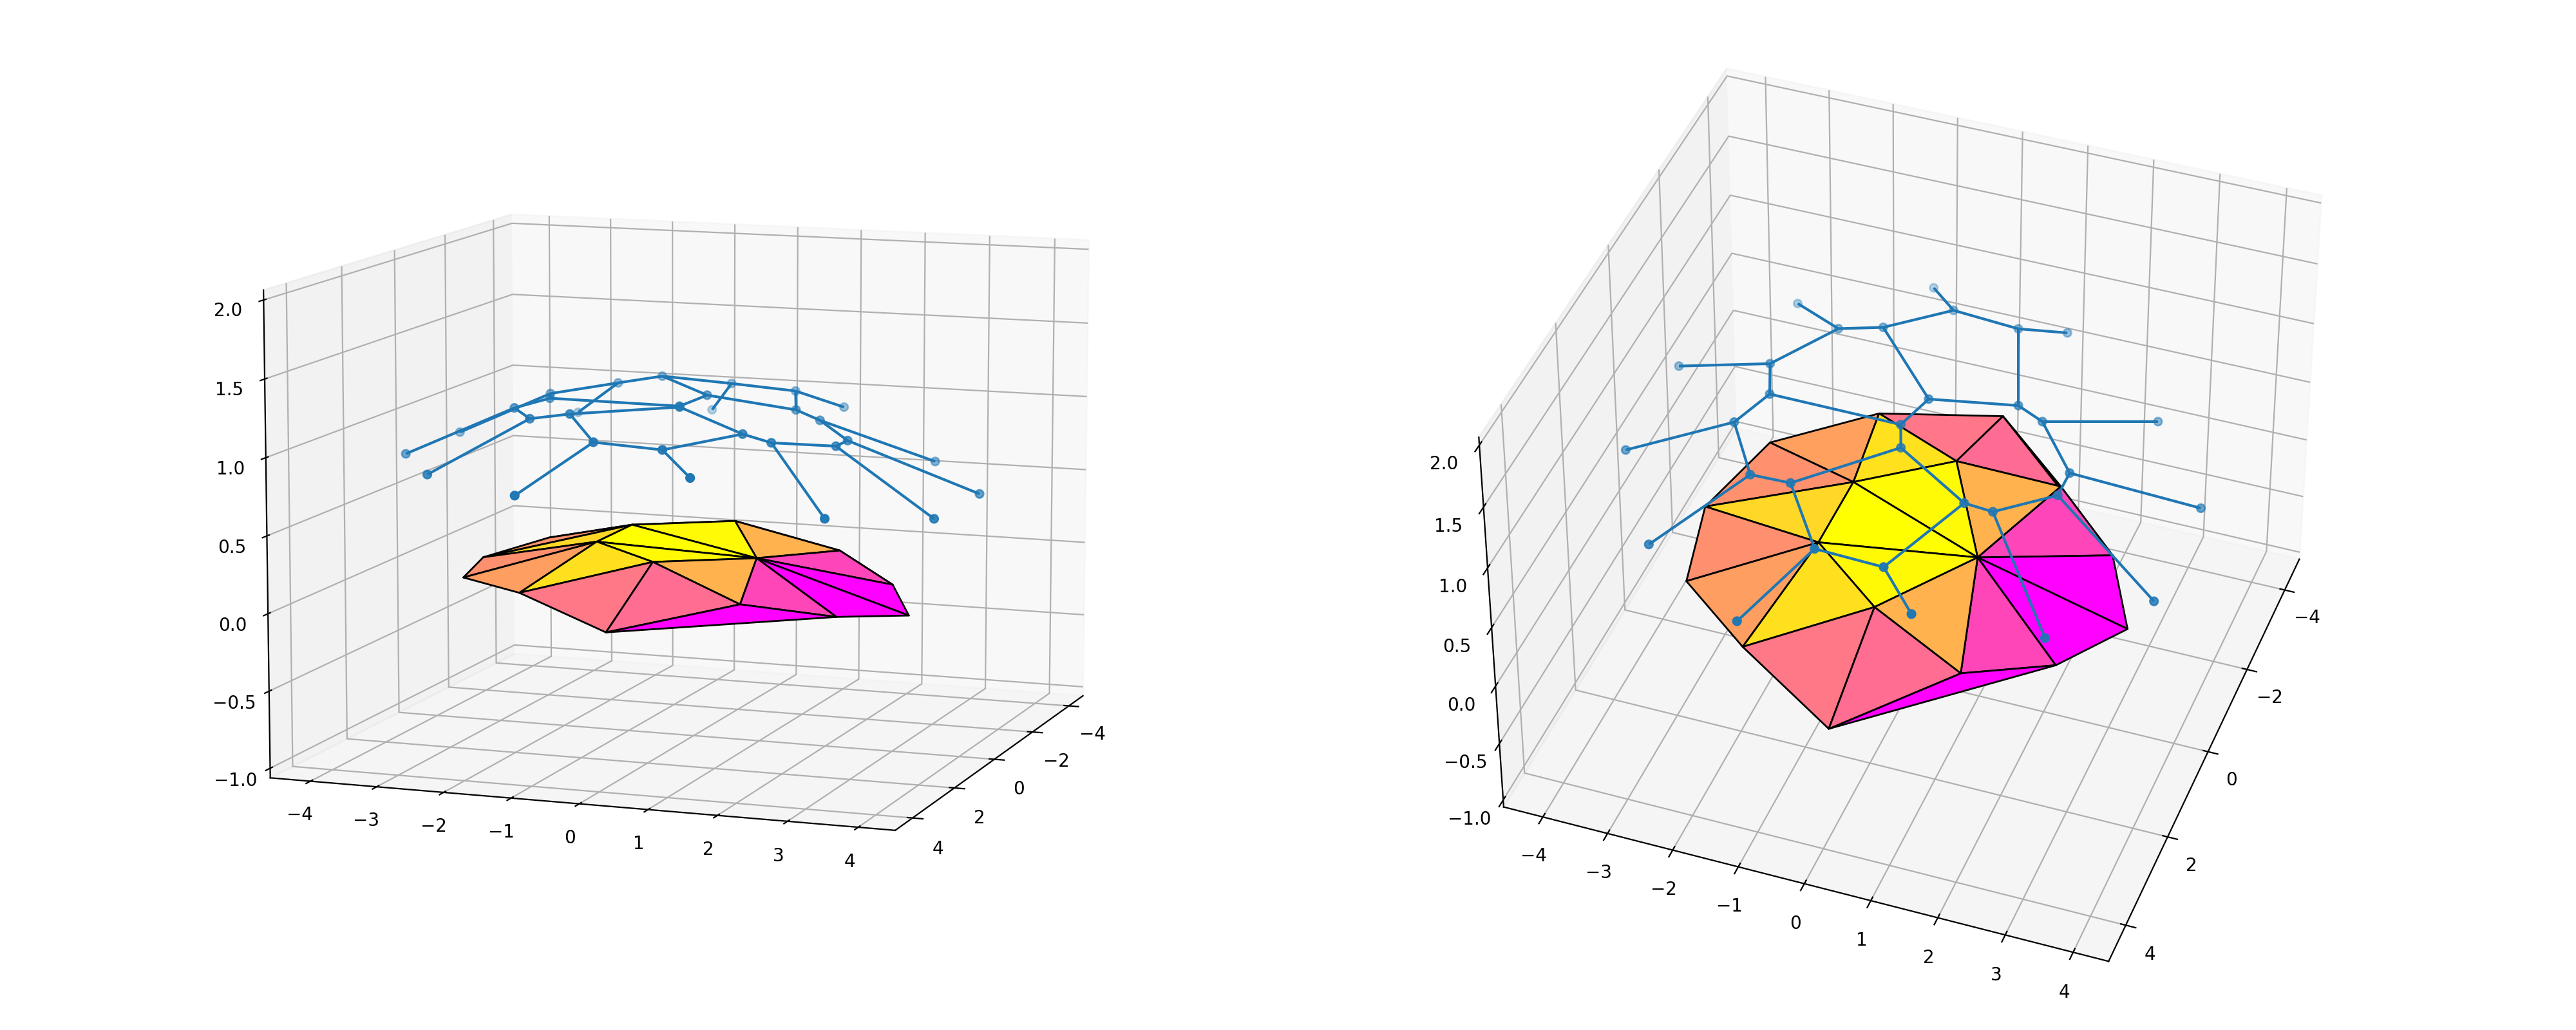
\includegraphics[width=0.69\textwidth]{kink/kink0.95_0.8_1.52_10_plot.png}
        \caption{Sheet shape when $\phi_0=0.95$, $\psi_0=0.8$, $\ell_0=1.52$.}
        \label{subfig:kink_out}
    \end{subfigure}
    \caption{Cell sheet geometry with a node of degree 7. The graph topology is affected in the sheet interior (subfigure \ref{subfig:kink_graph}). This minor change has substantial effects on the sheet geometry (subfigures \ref{subfig:kink_in}, \ref{subfig:kink_out}).}
    \label{fig:kink}
\end{figure}

\begin{figure}[htbp]
    \centering
    \begin{subfigure}[b]{\textwidth}
        \centering
        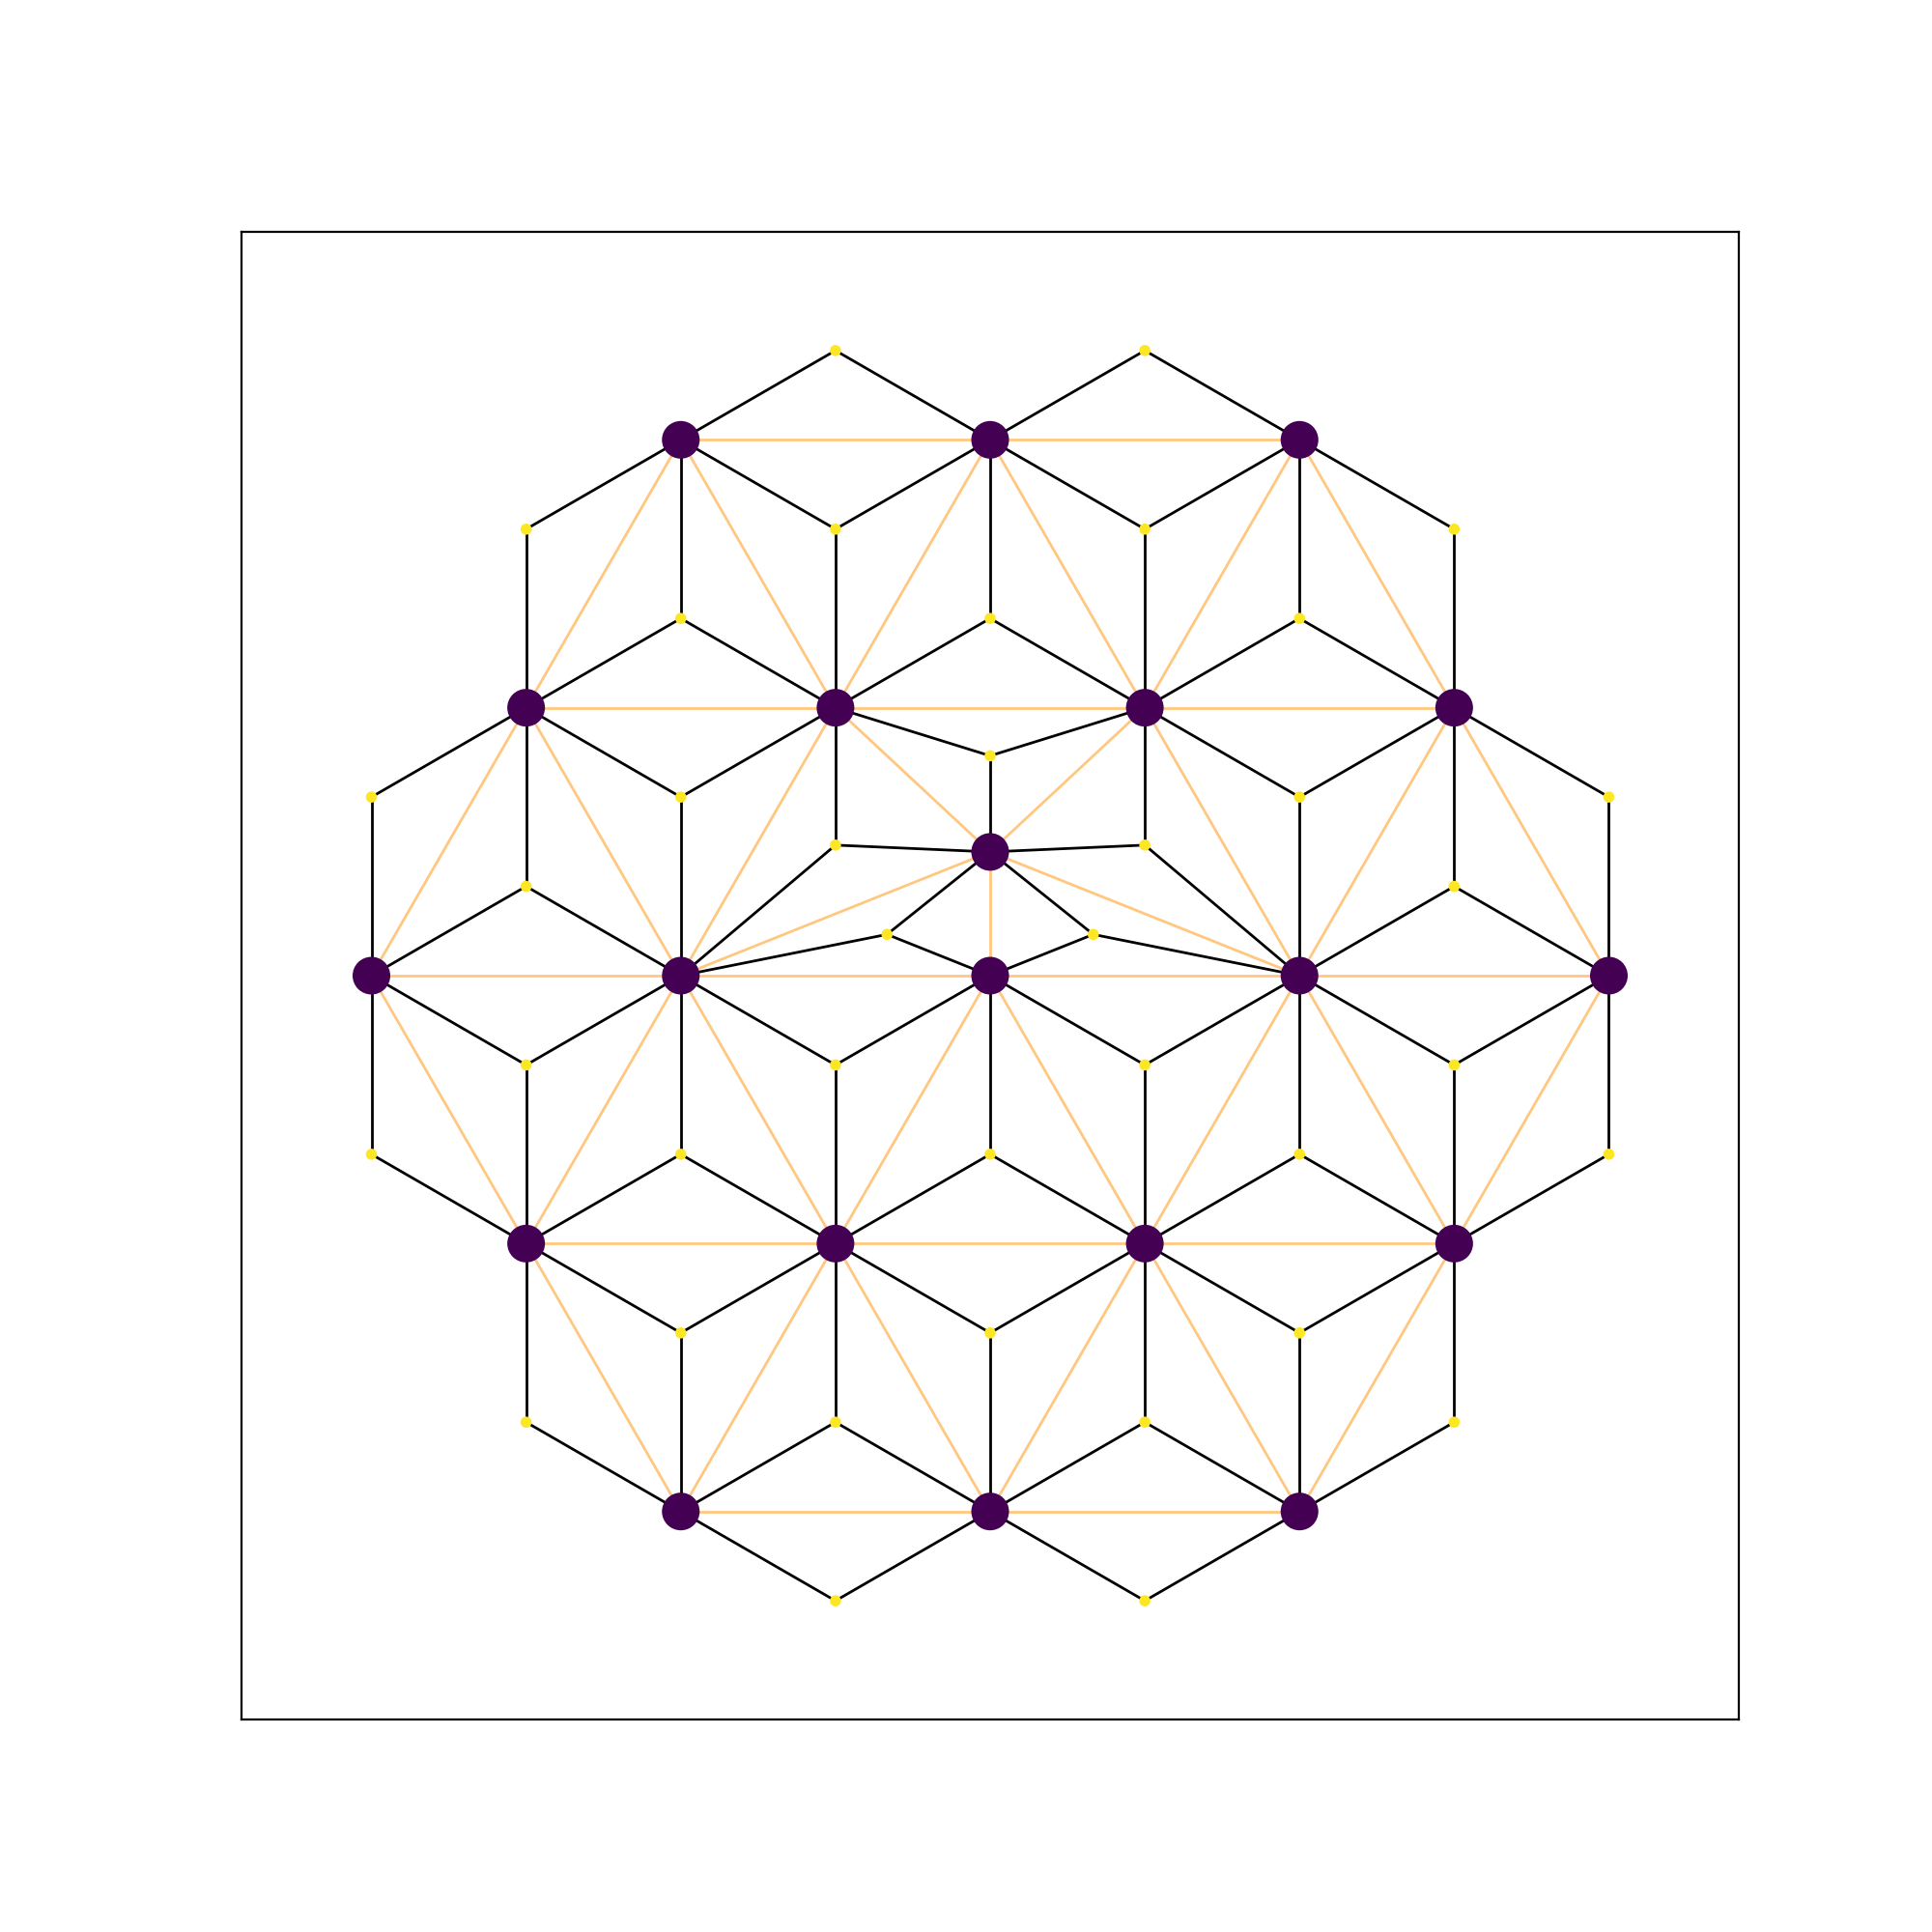
\includegraphics[width=0.5\textwidth]{bump/bump_graph.png}
        \caption{Initial lattice drawn as in Figure \ref{fig:layout_init}.}
        \label{subfig:bump_graph}
    \end{subfigure}
    \begin{subfigure}[b]{\textwidth}
        \centering
        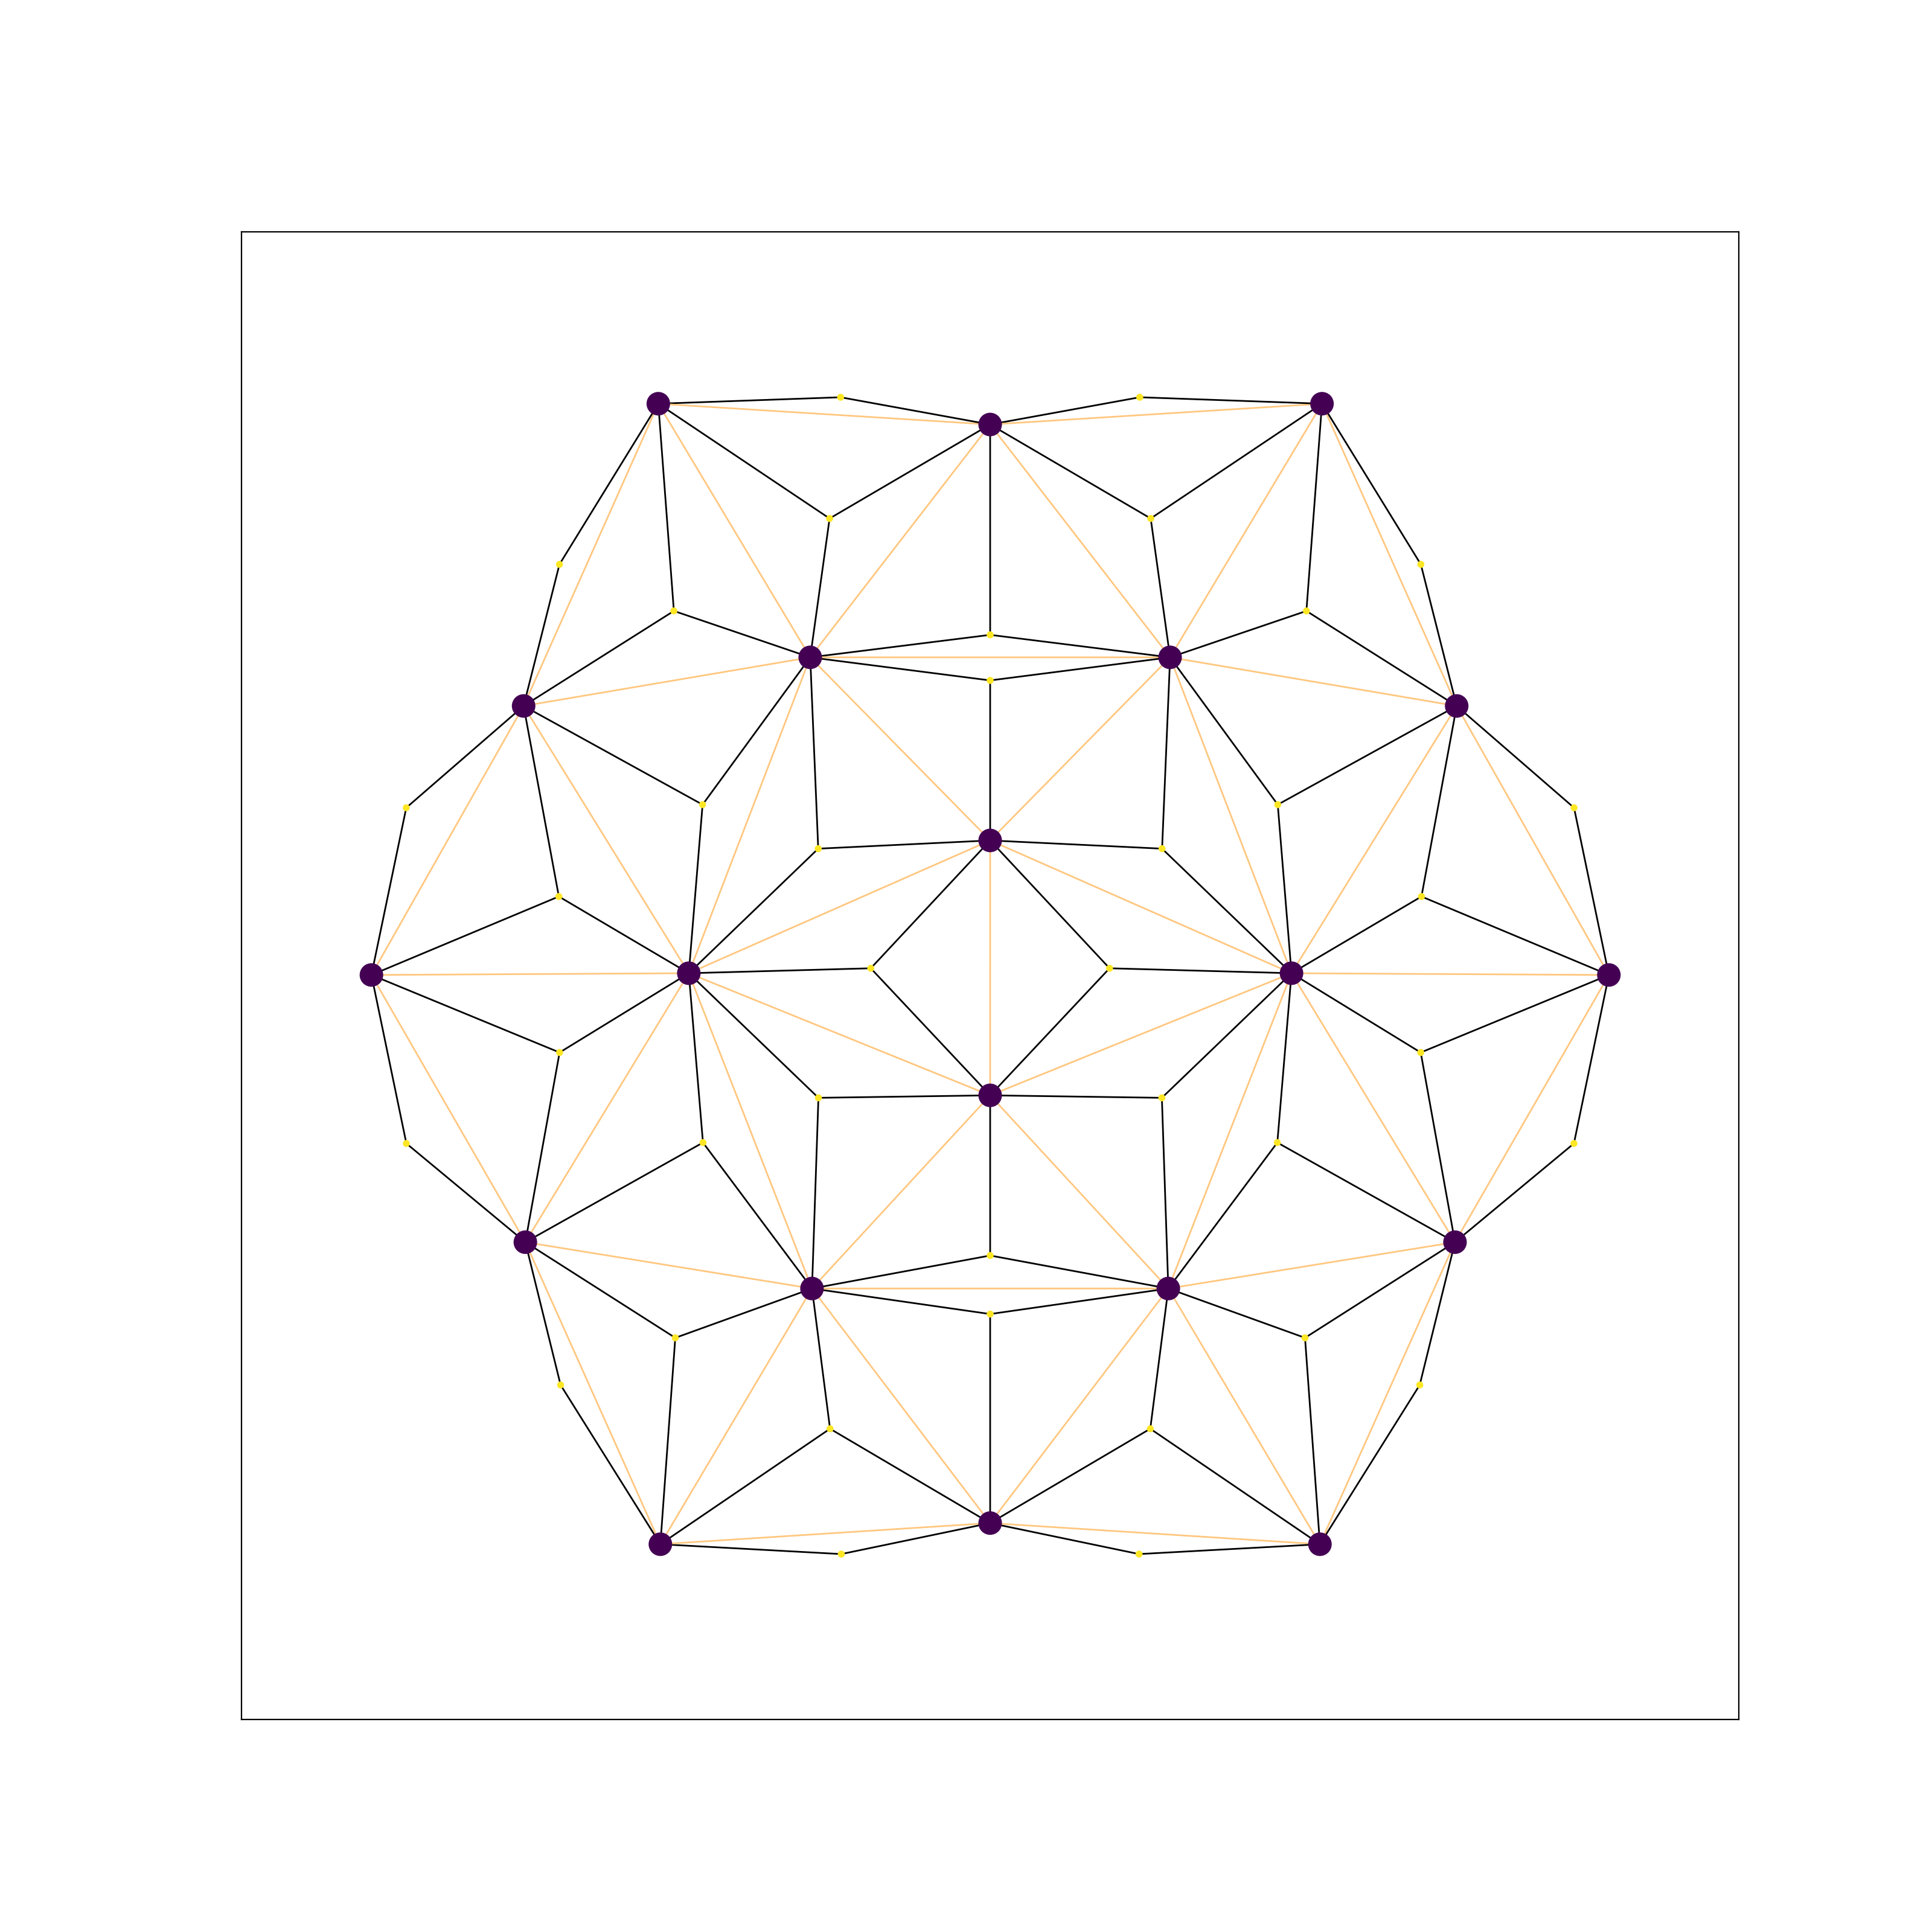
\includegraphics[width=0.3\textwidth]{bump/bump0.8_0.8_1.52_10_graph.png}
        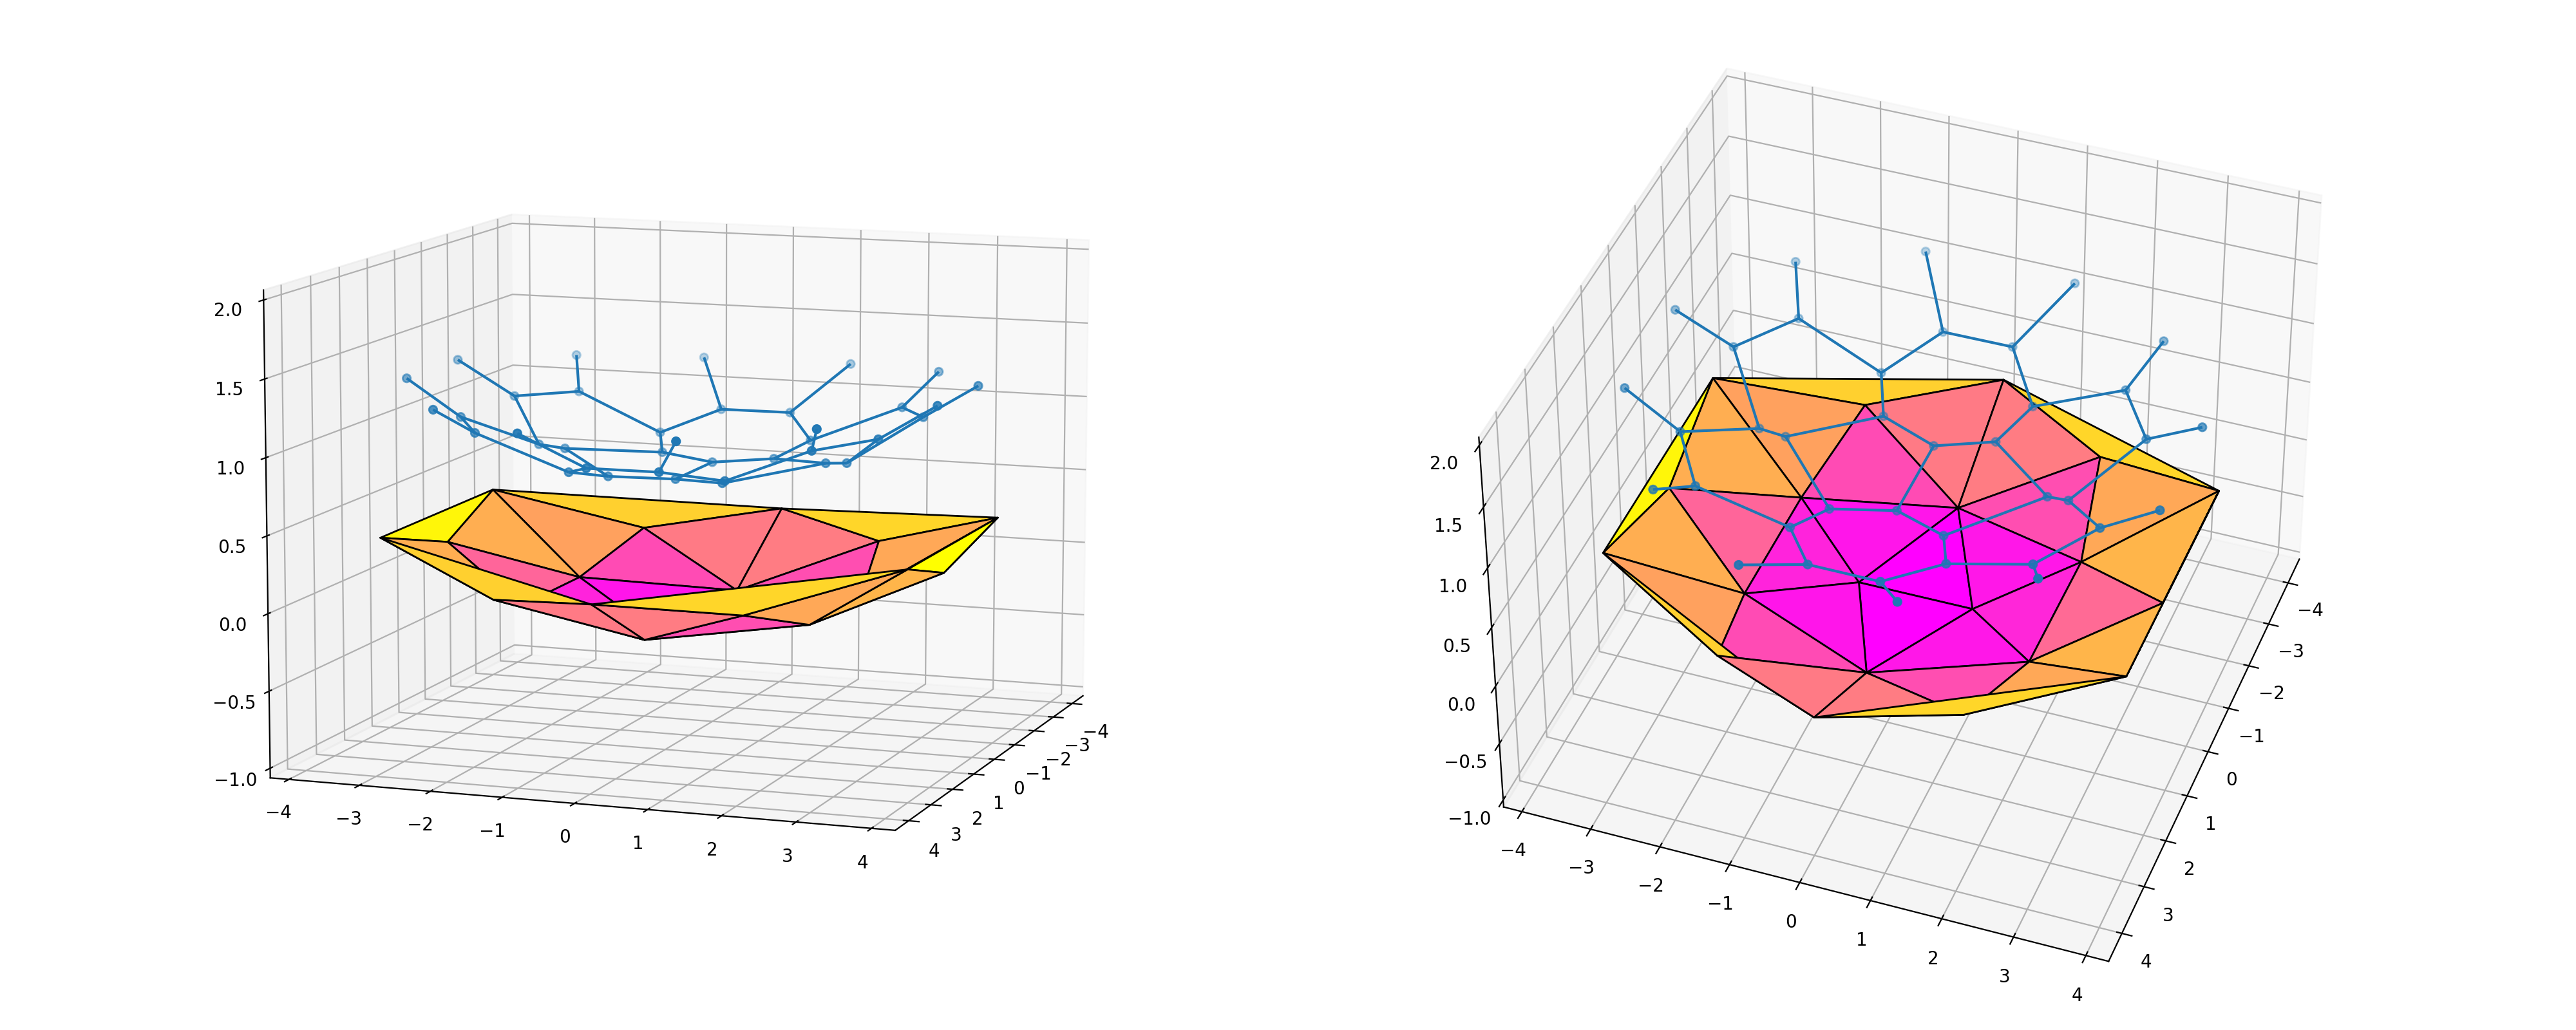
\includegraphics[width=0.69\textwidth]{bump/bump0.8_0.8_1.52_10_plot.png}
        \caption{Sheet shape when $\phi_0=0.8$, $\psi_0=0.8$, $\ell_0=1.52$.}
        \label{subfig:bump_in}
    \end{subfigure}
    \begin{subfigure}[b]{\textwidth}
        \centering
        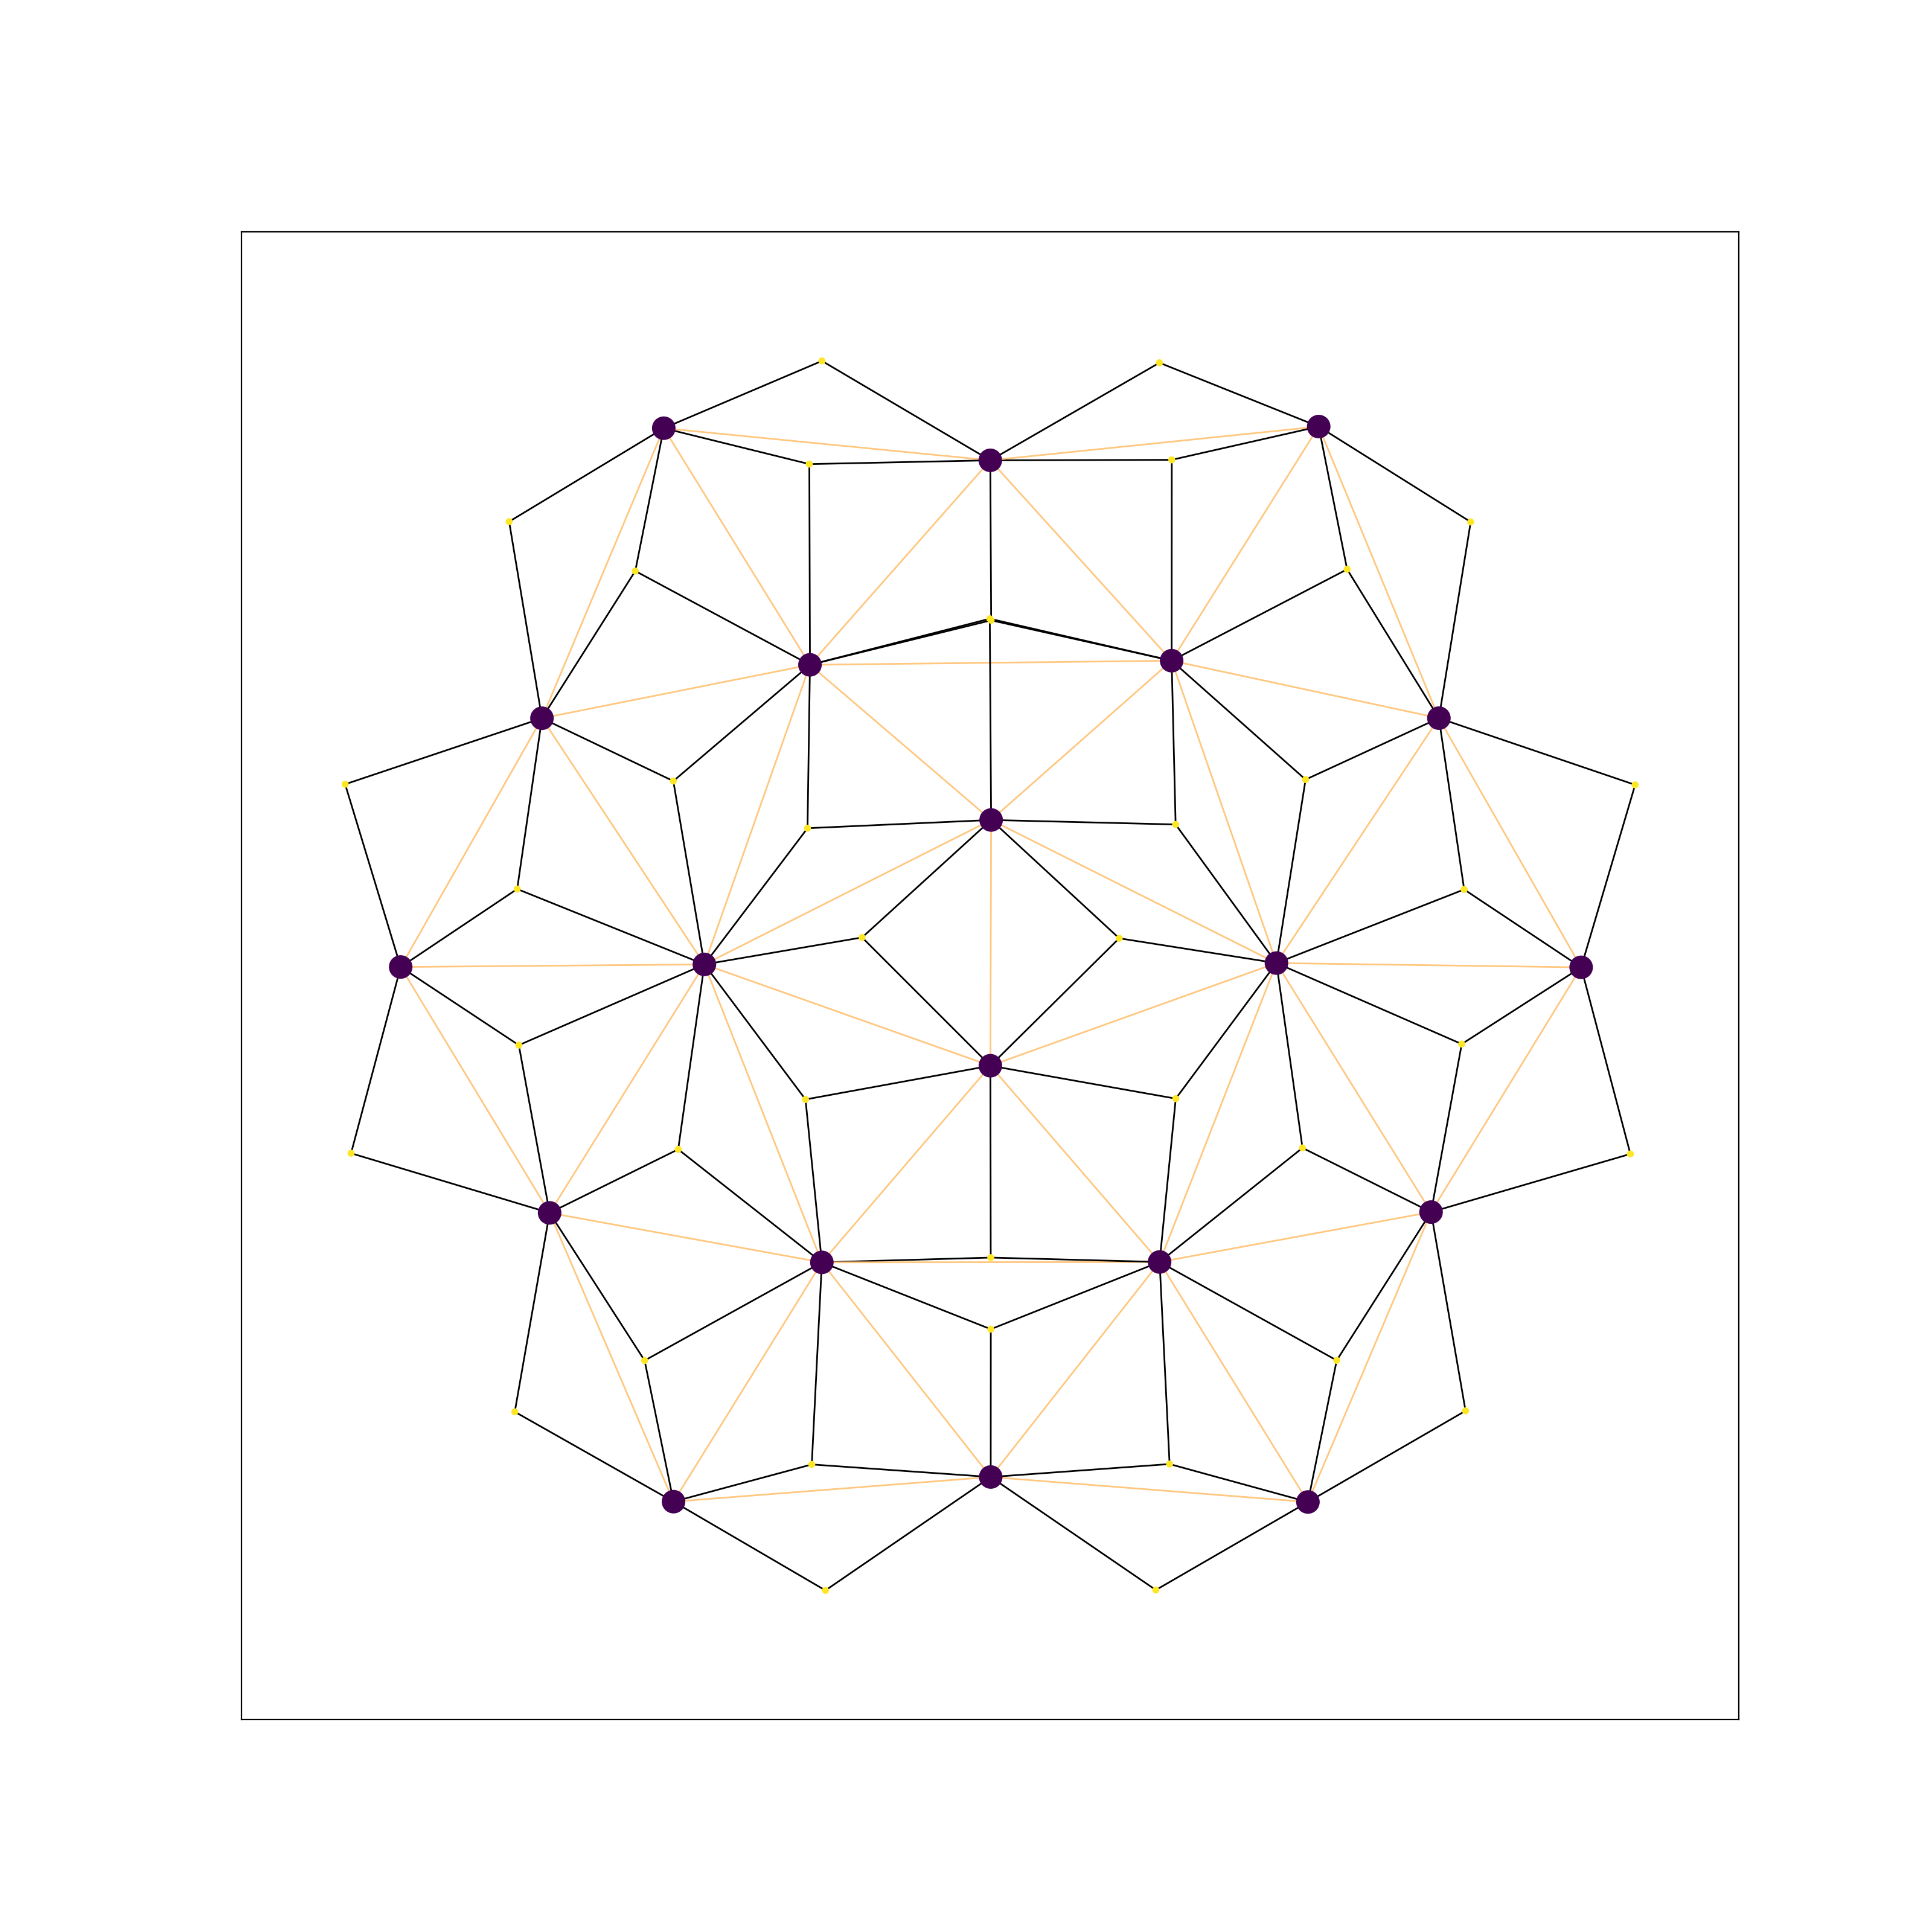
\includegraphics[width=0.3\textwidth]{bump/bump0.95_0.8_1.52_10_graph.png}
        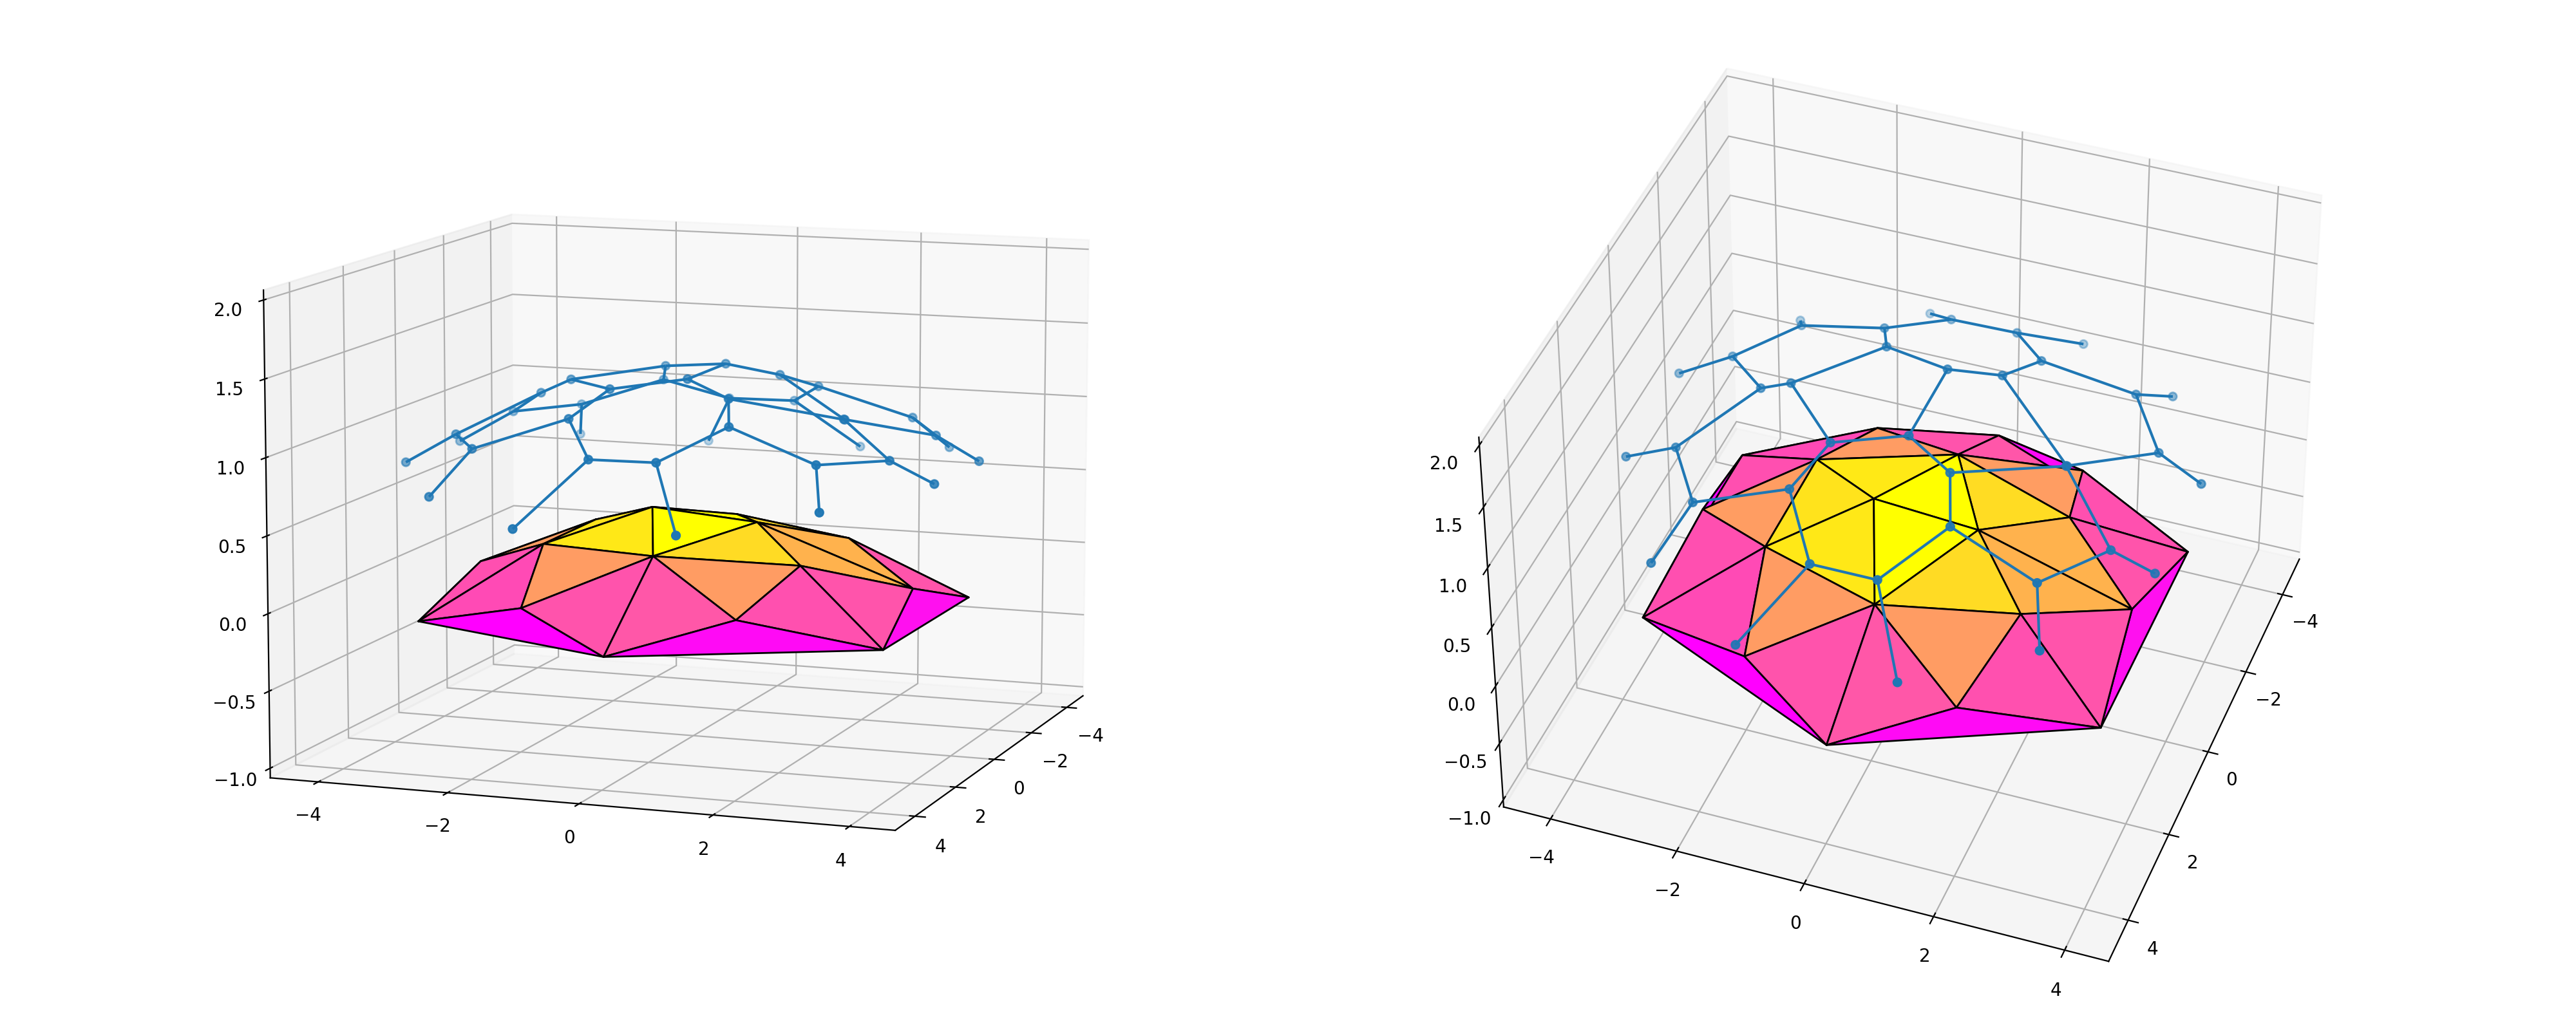
\includegraphics[width=0.69\textwidth]{bump/bump0.95_0.8_1.52_10_plot.png}
        \caption{Sheet shape when $\phi_0=0.95$, $\psi_0=0.8$, $\ell_0=1.52$.}
        \label{subfig:bump_out}
    \end{subfigure}
    \caption{Cell sheet geometry with a node of degree 7. The graph topology is affected in the sheet interior (subfigure \ref{subfig:bump_graph}). This minor change has substantial effects on the sheet geometry (subfigures \ref{subfig:bump_in}, \ref{subfig:bump_out}).}
    \label{fig:bump}
\end{figure}

\subsection{Larger cell sheets}

If if inverting a sheet of cells involves flattening it out at the edges, then a small sheet will be able to do this easier than a large one. This is because the cells on the outside have to stretch their collars less if the sheet is smaller when they flatten out. 

\begin{figure}[htbp]
    \centering
    \begin{subfigure}[b]{\textwidth}
        \centering
        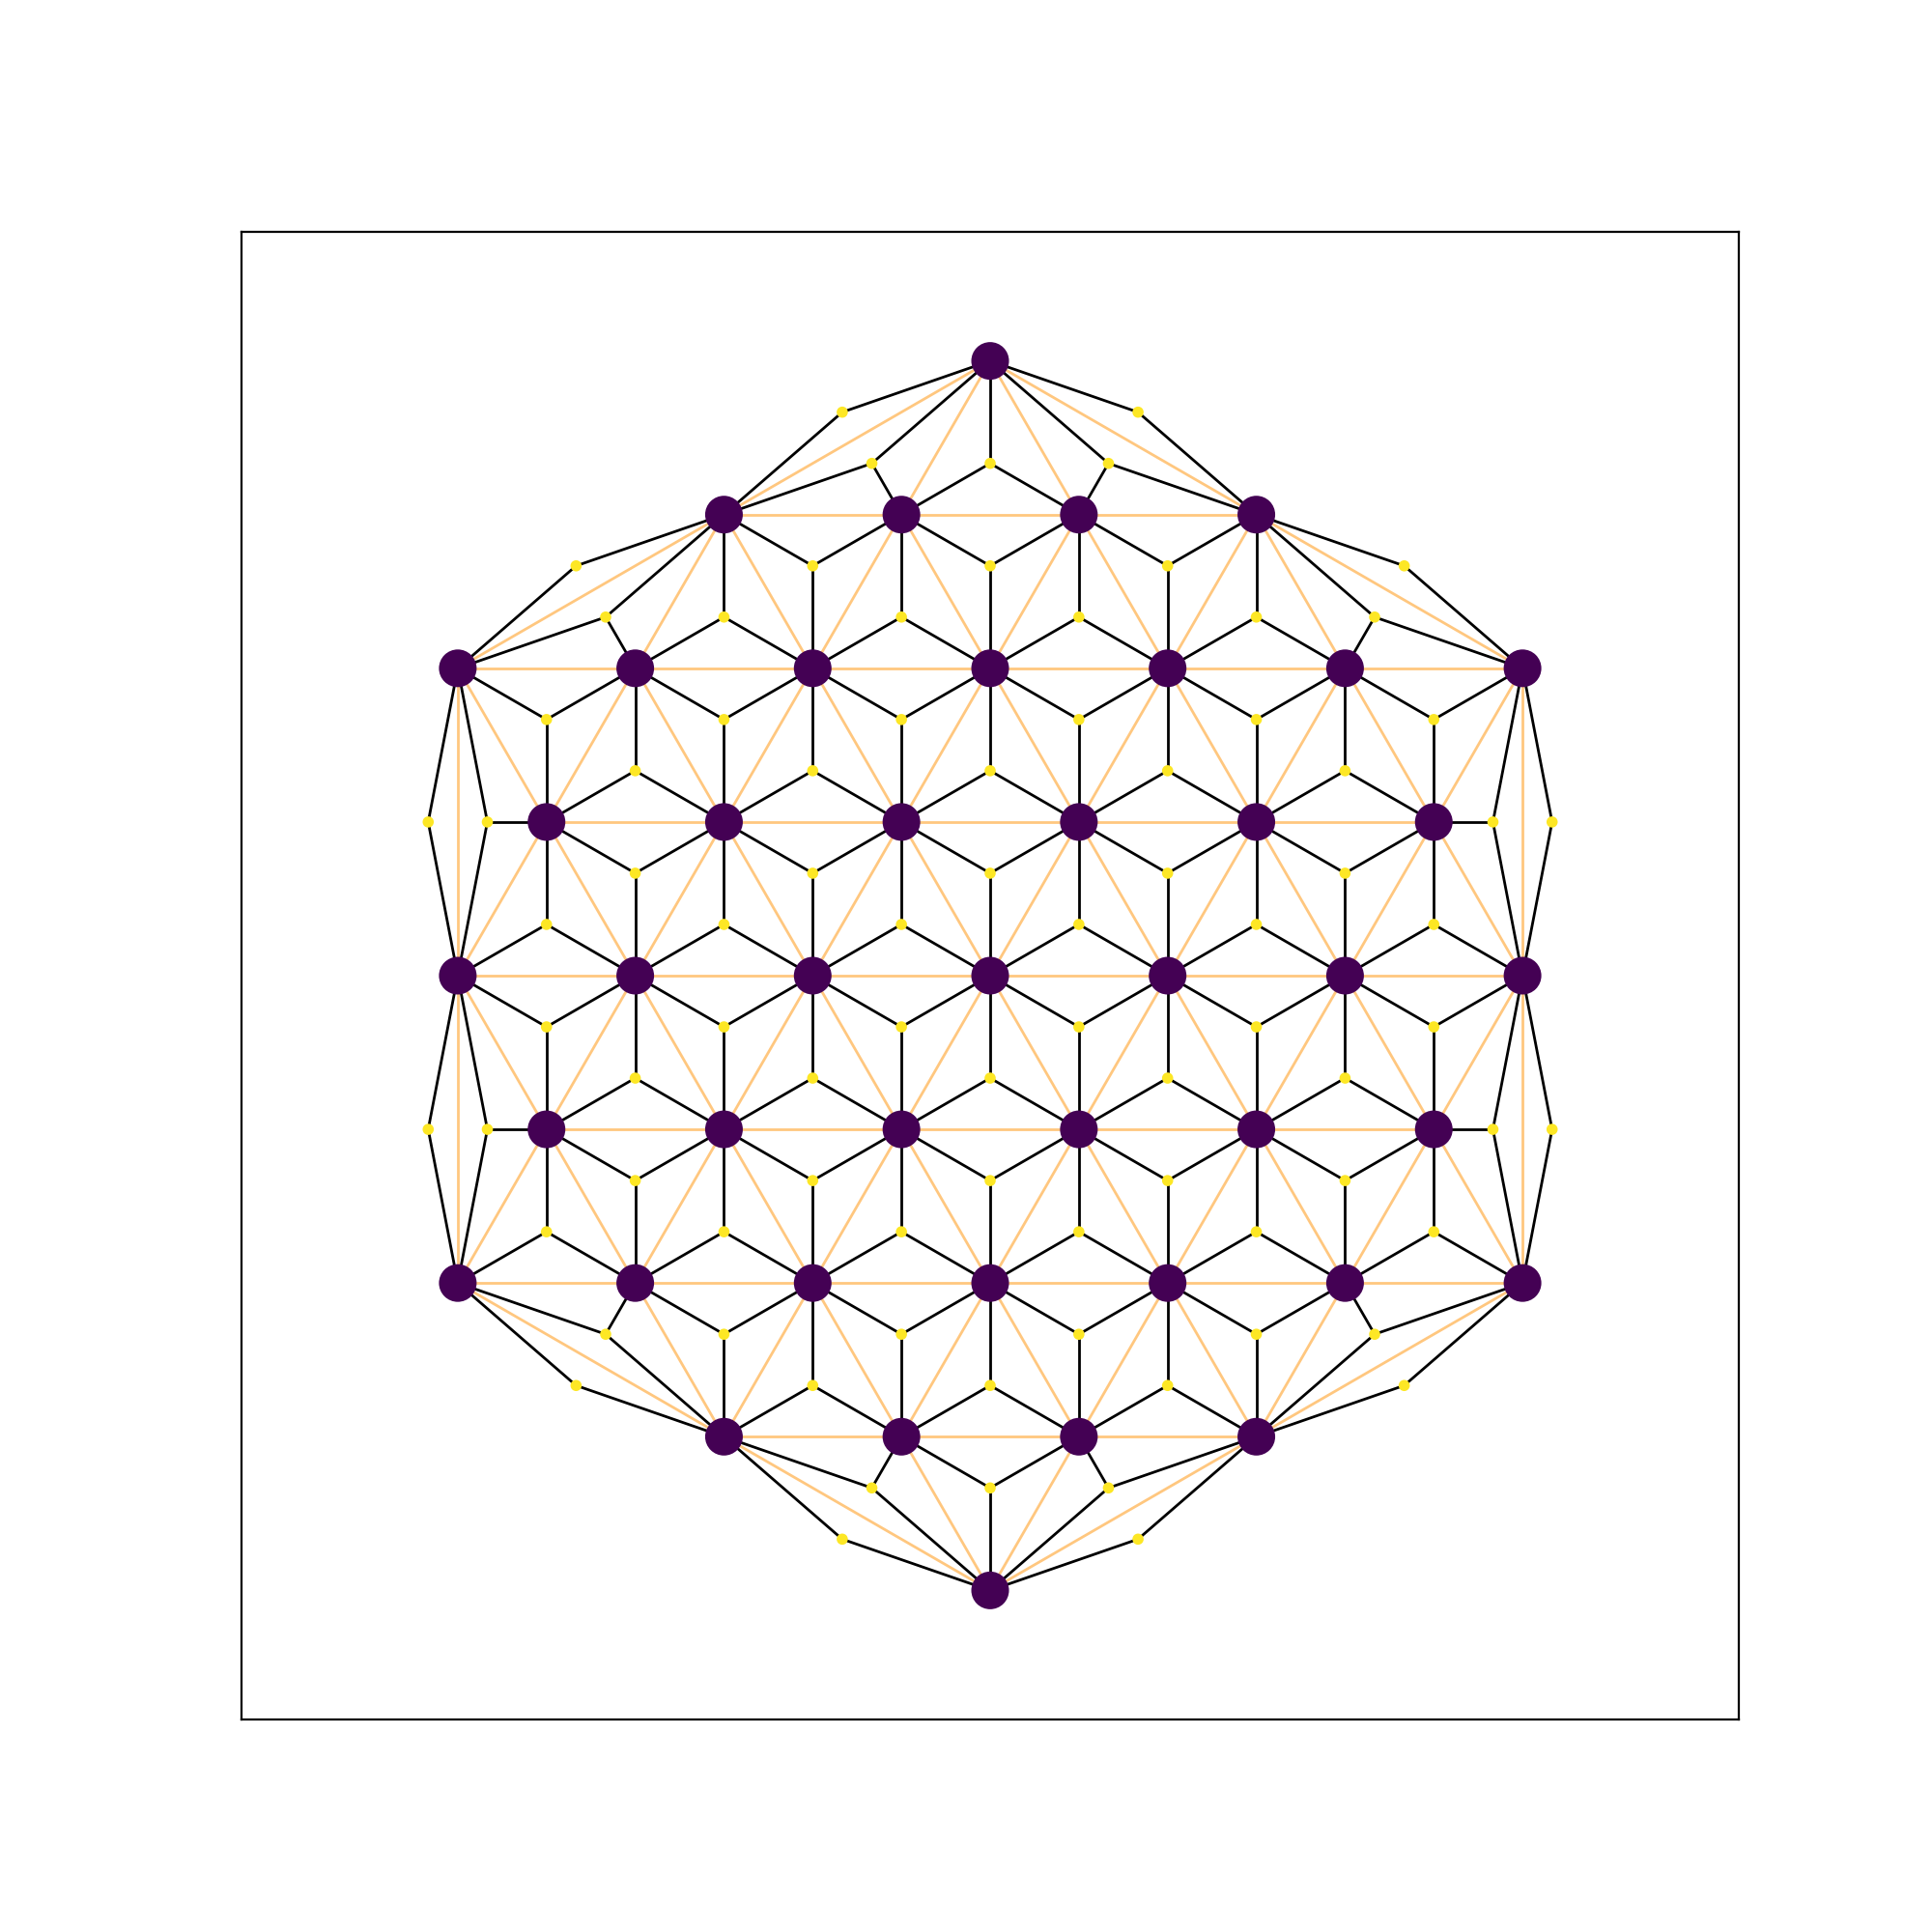
\includegraphics[width=0.5\textwidth]{hexbig/hexbig_graph.png}
        \caption{Initial lattice drawn as in Figure \ref{fig:layout_init}.}
        \label{subfig:hexbig_graph}
    \end{subfigure}
    \begin{subfigure}[b]{\textwidth}
        \centering
        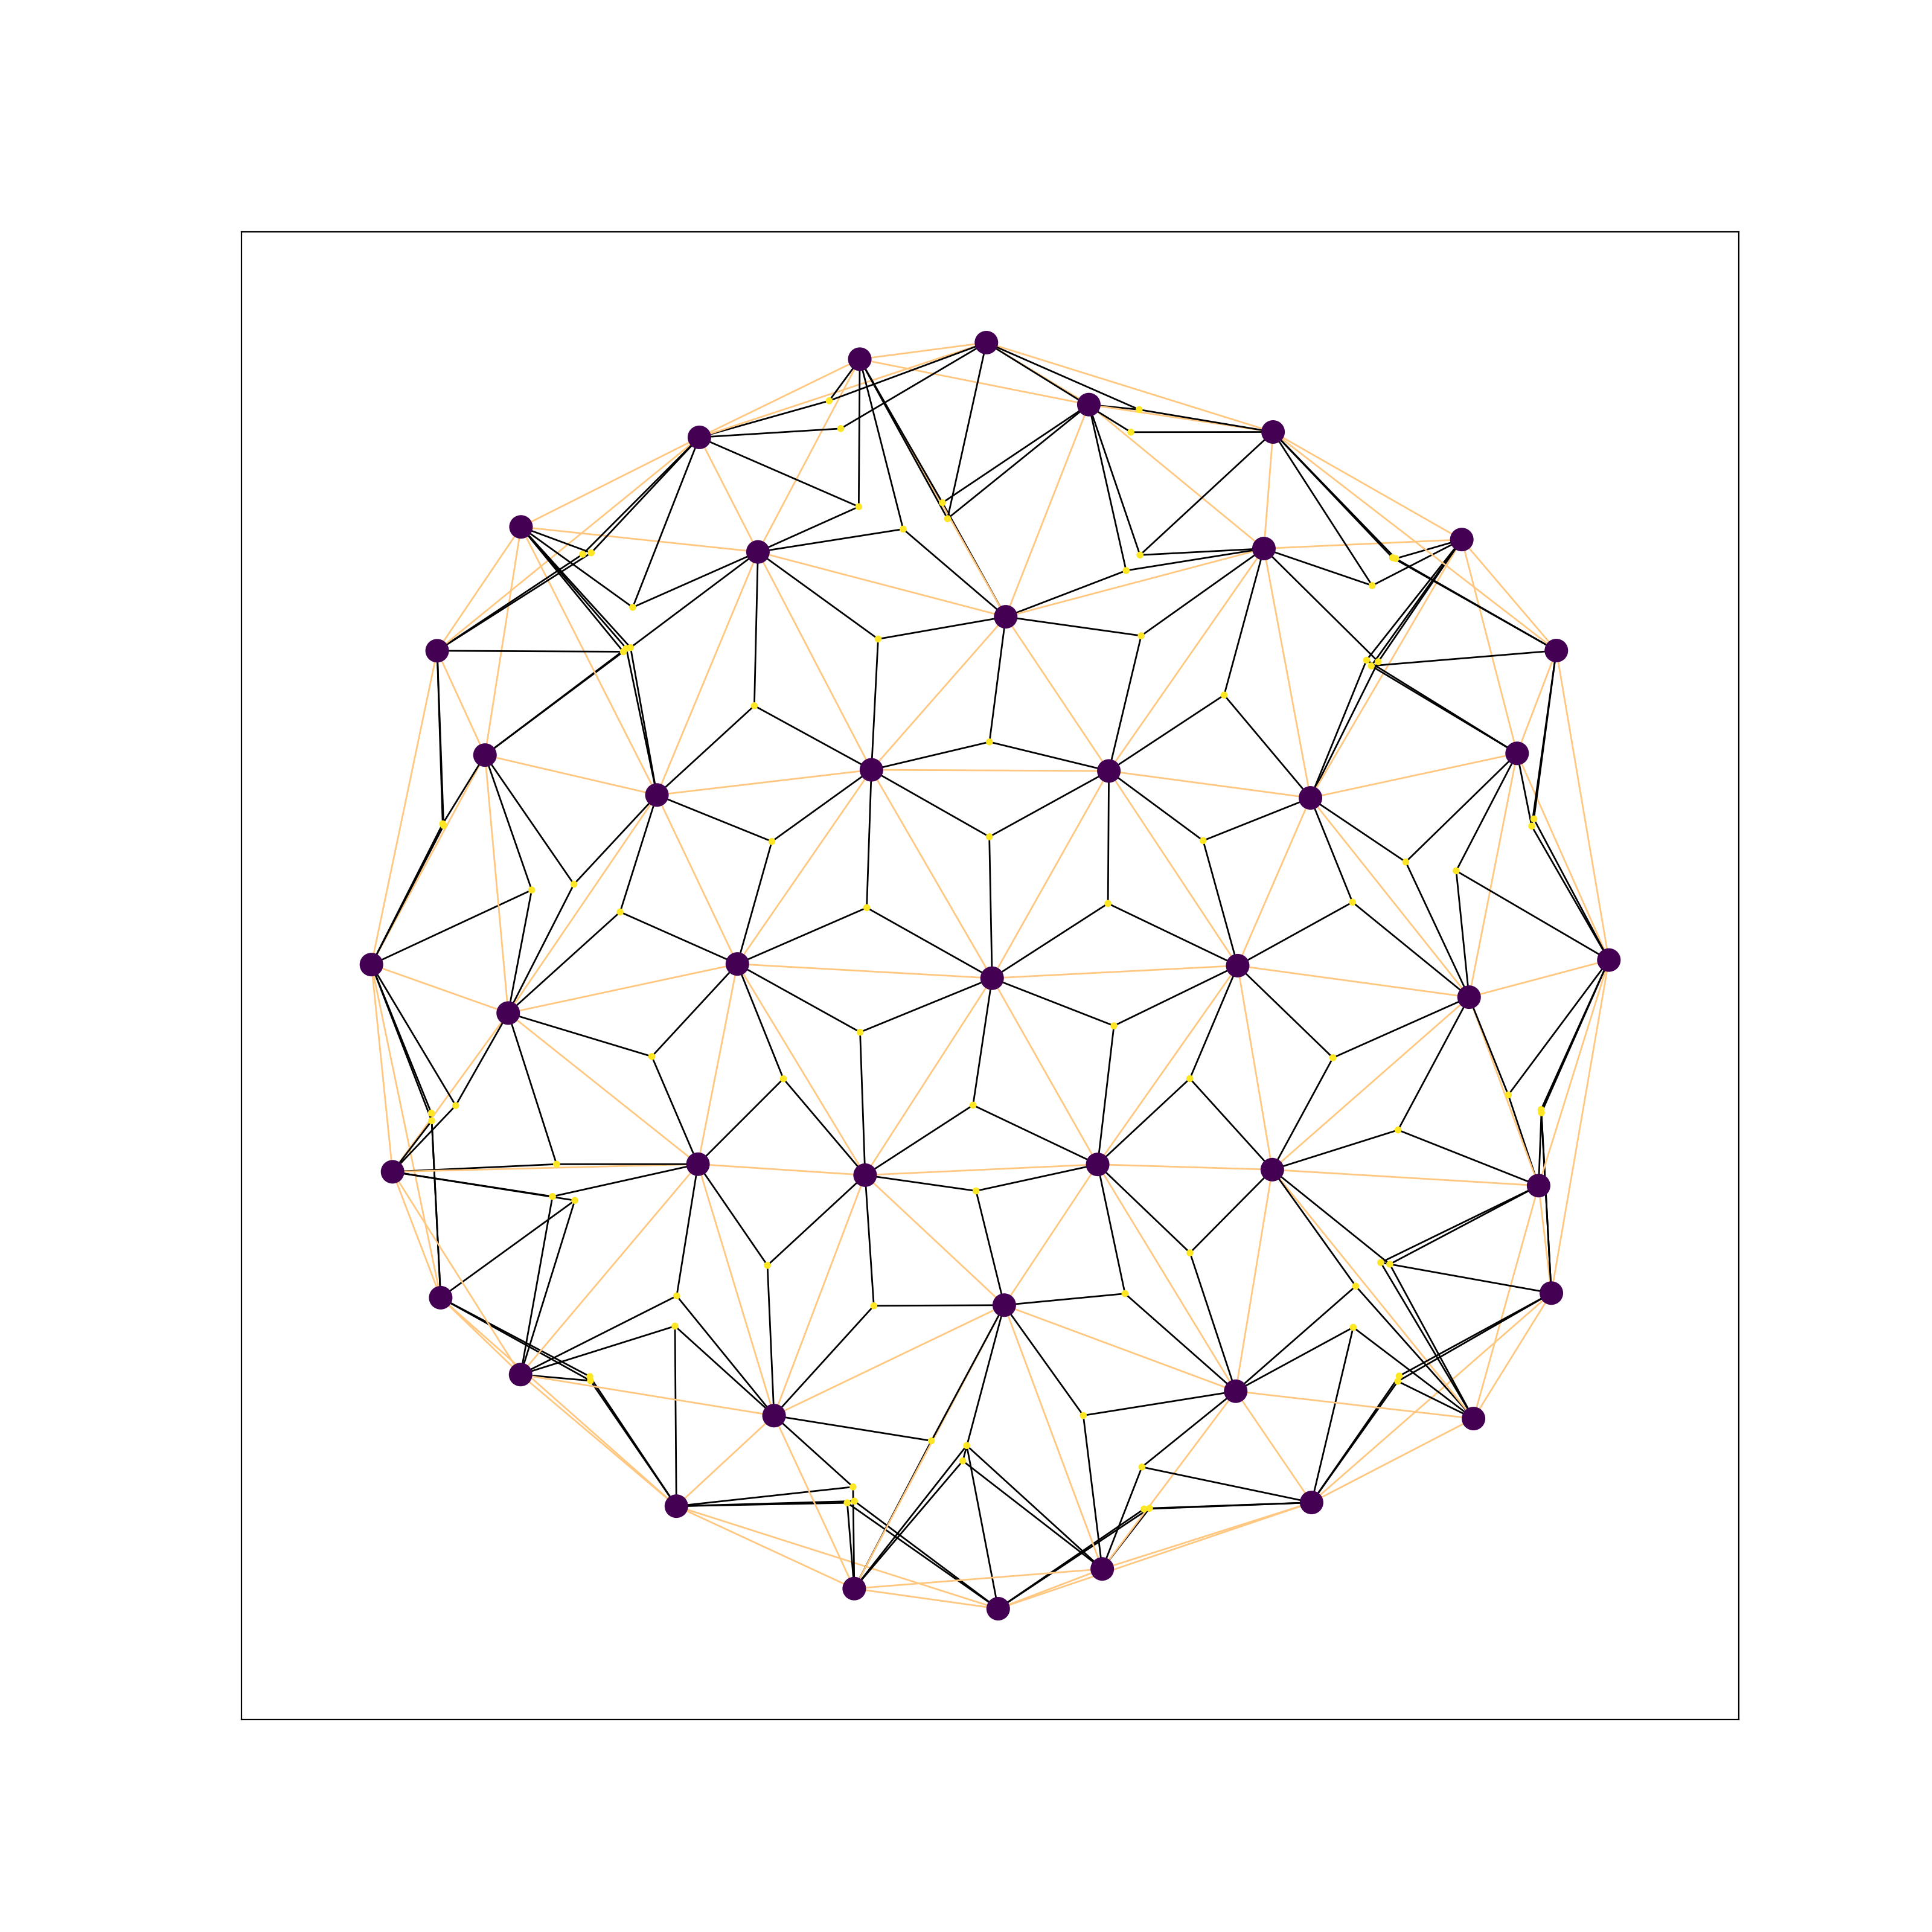
\includegraphics[width=0.3\textwidth]{hexbig/hexbig0.8_0.8_1.35_10_graph.png}
        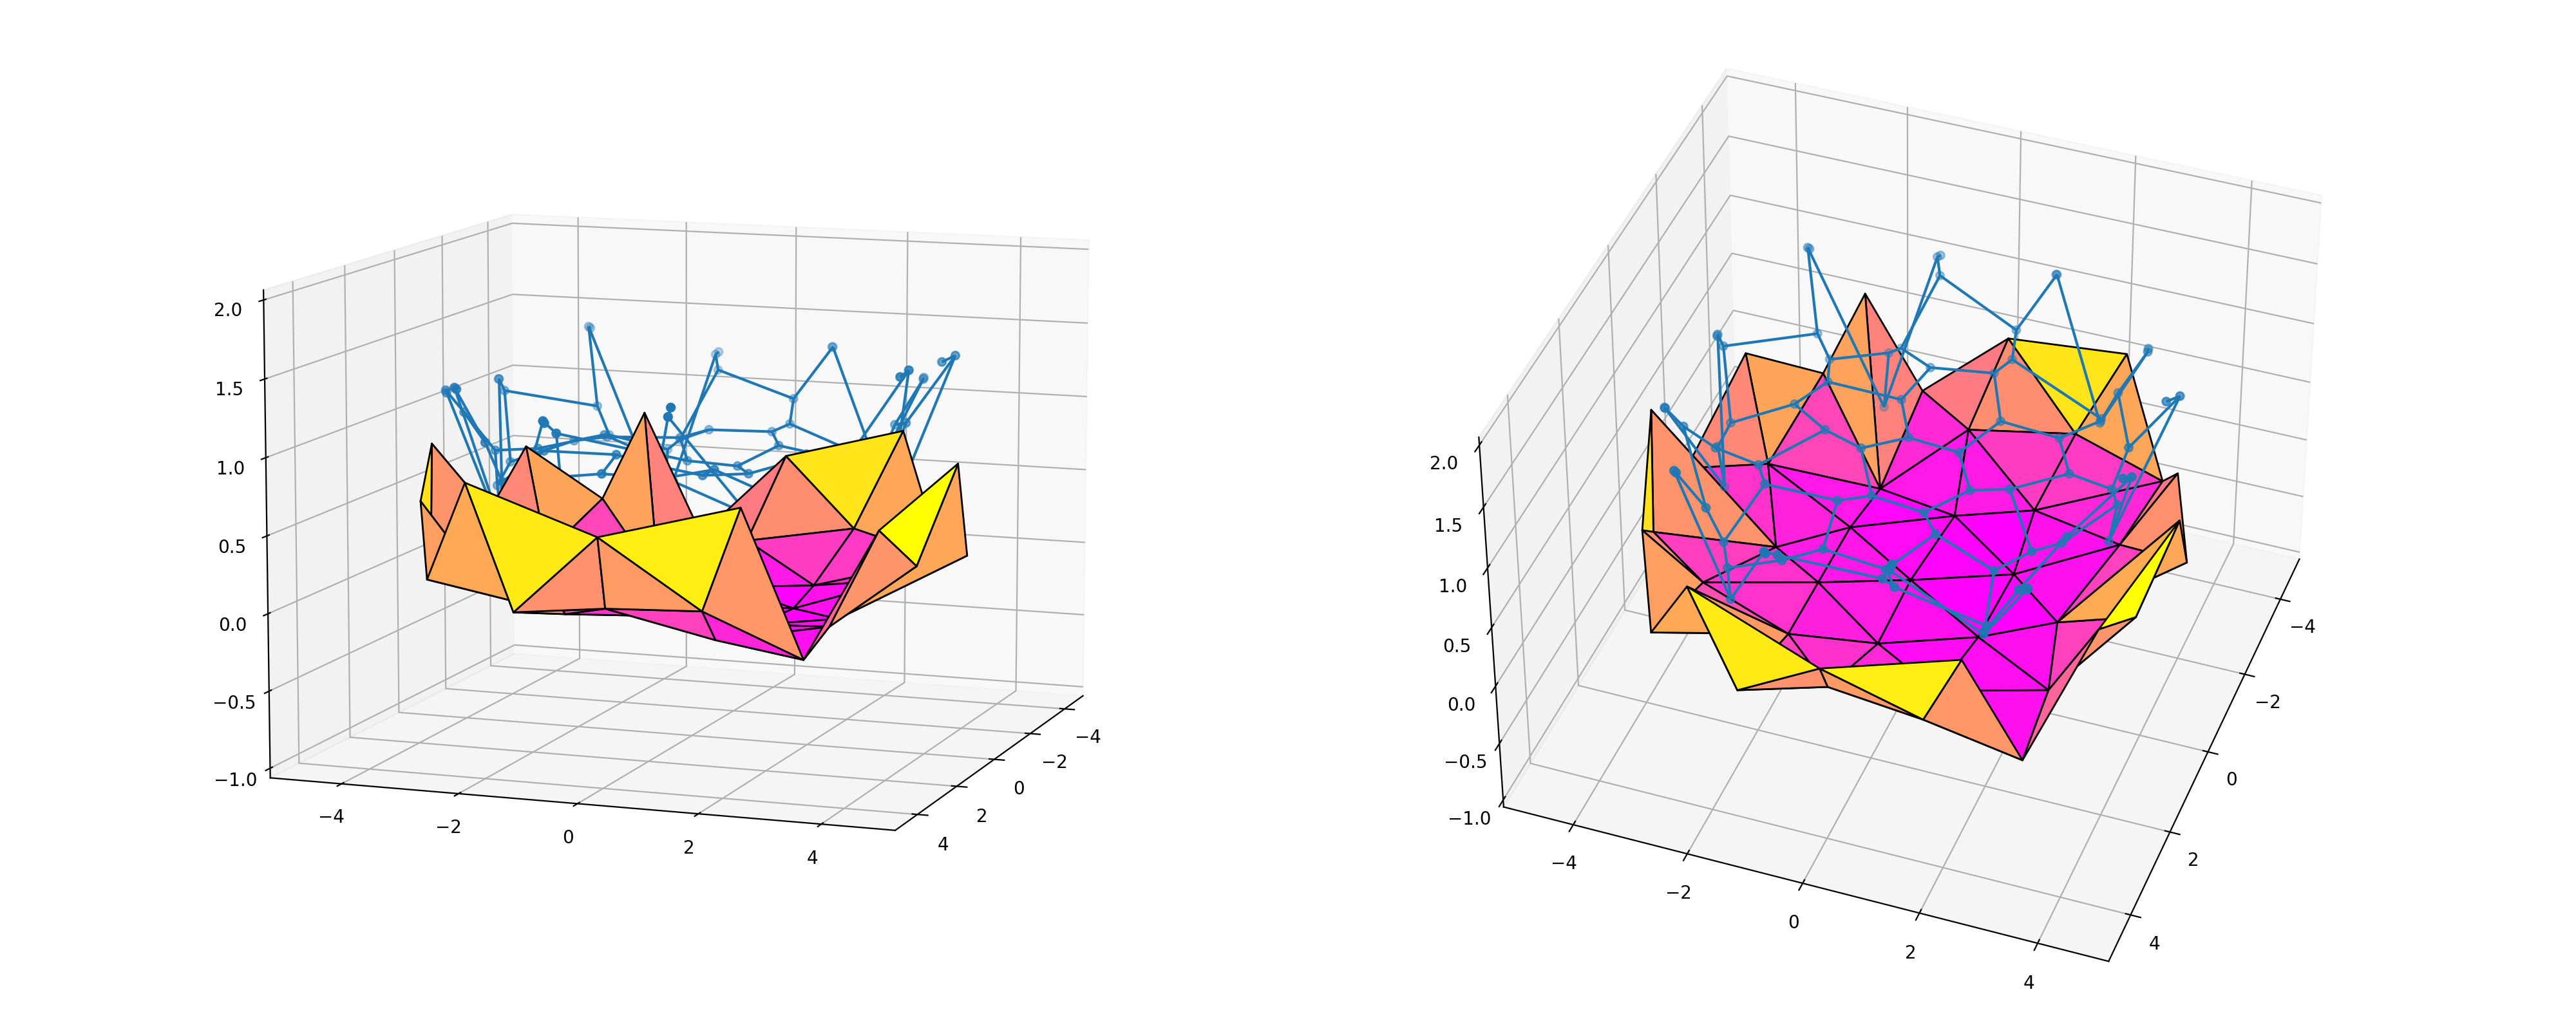
\includegraphics[width=0.69\textwidth]{hexbig/hexbig0.8_0.8_1.35_10_plot.png}
        \caption{Sheet shape when $\phi_0=0.8$, $\psi_0=0.8$, $\ell_0=1.52$.}
        \label{subfig:hexbig_in}
    \end{subfigure}
    \begin{subfigure}[b]{\textwidth}
        \centering
        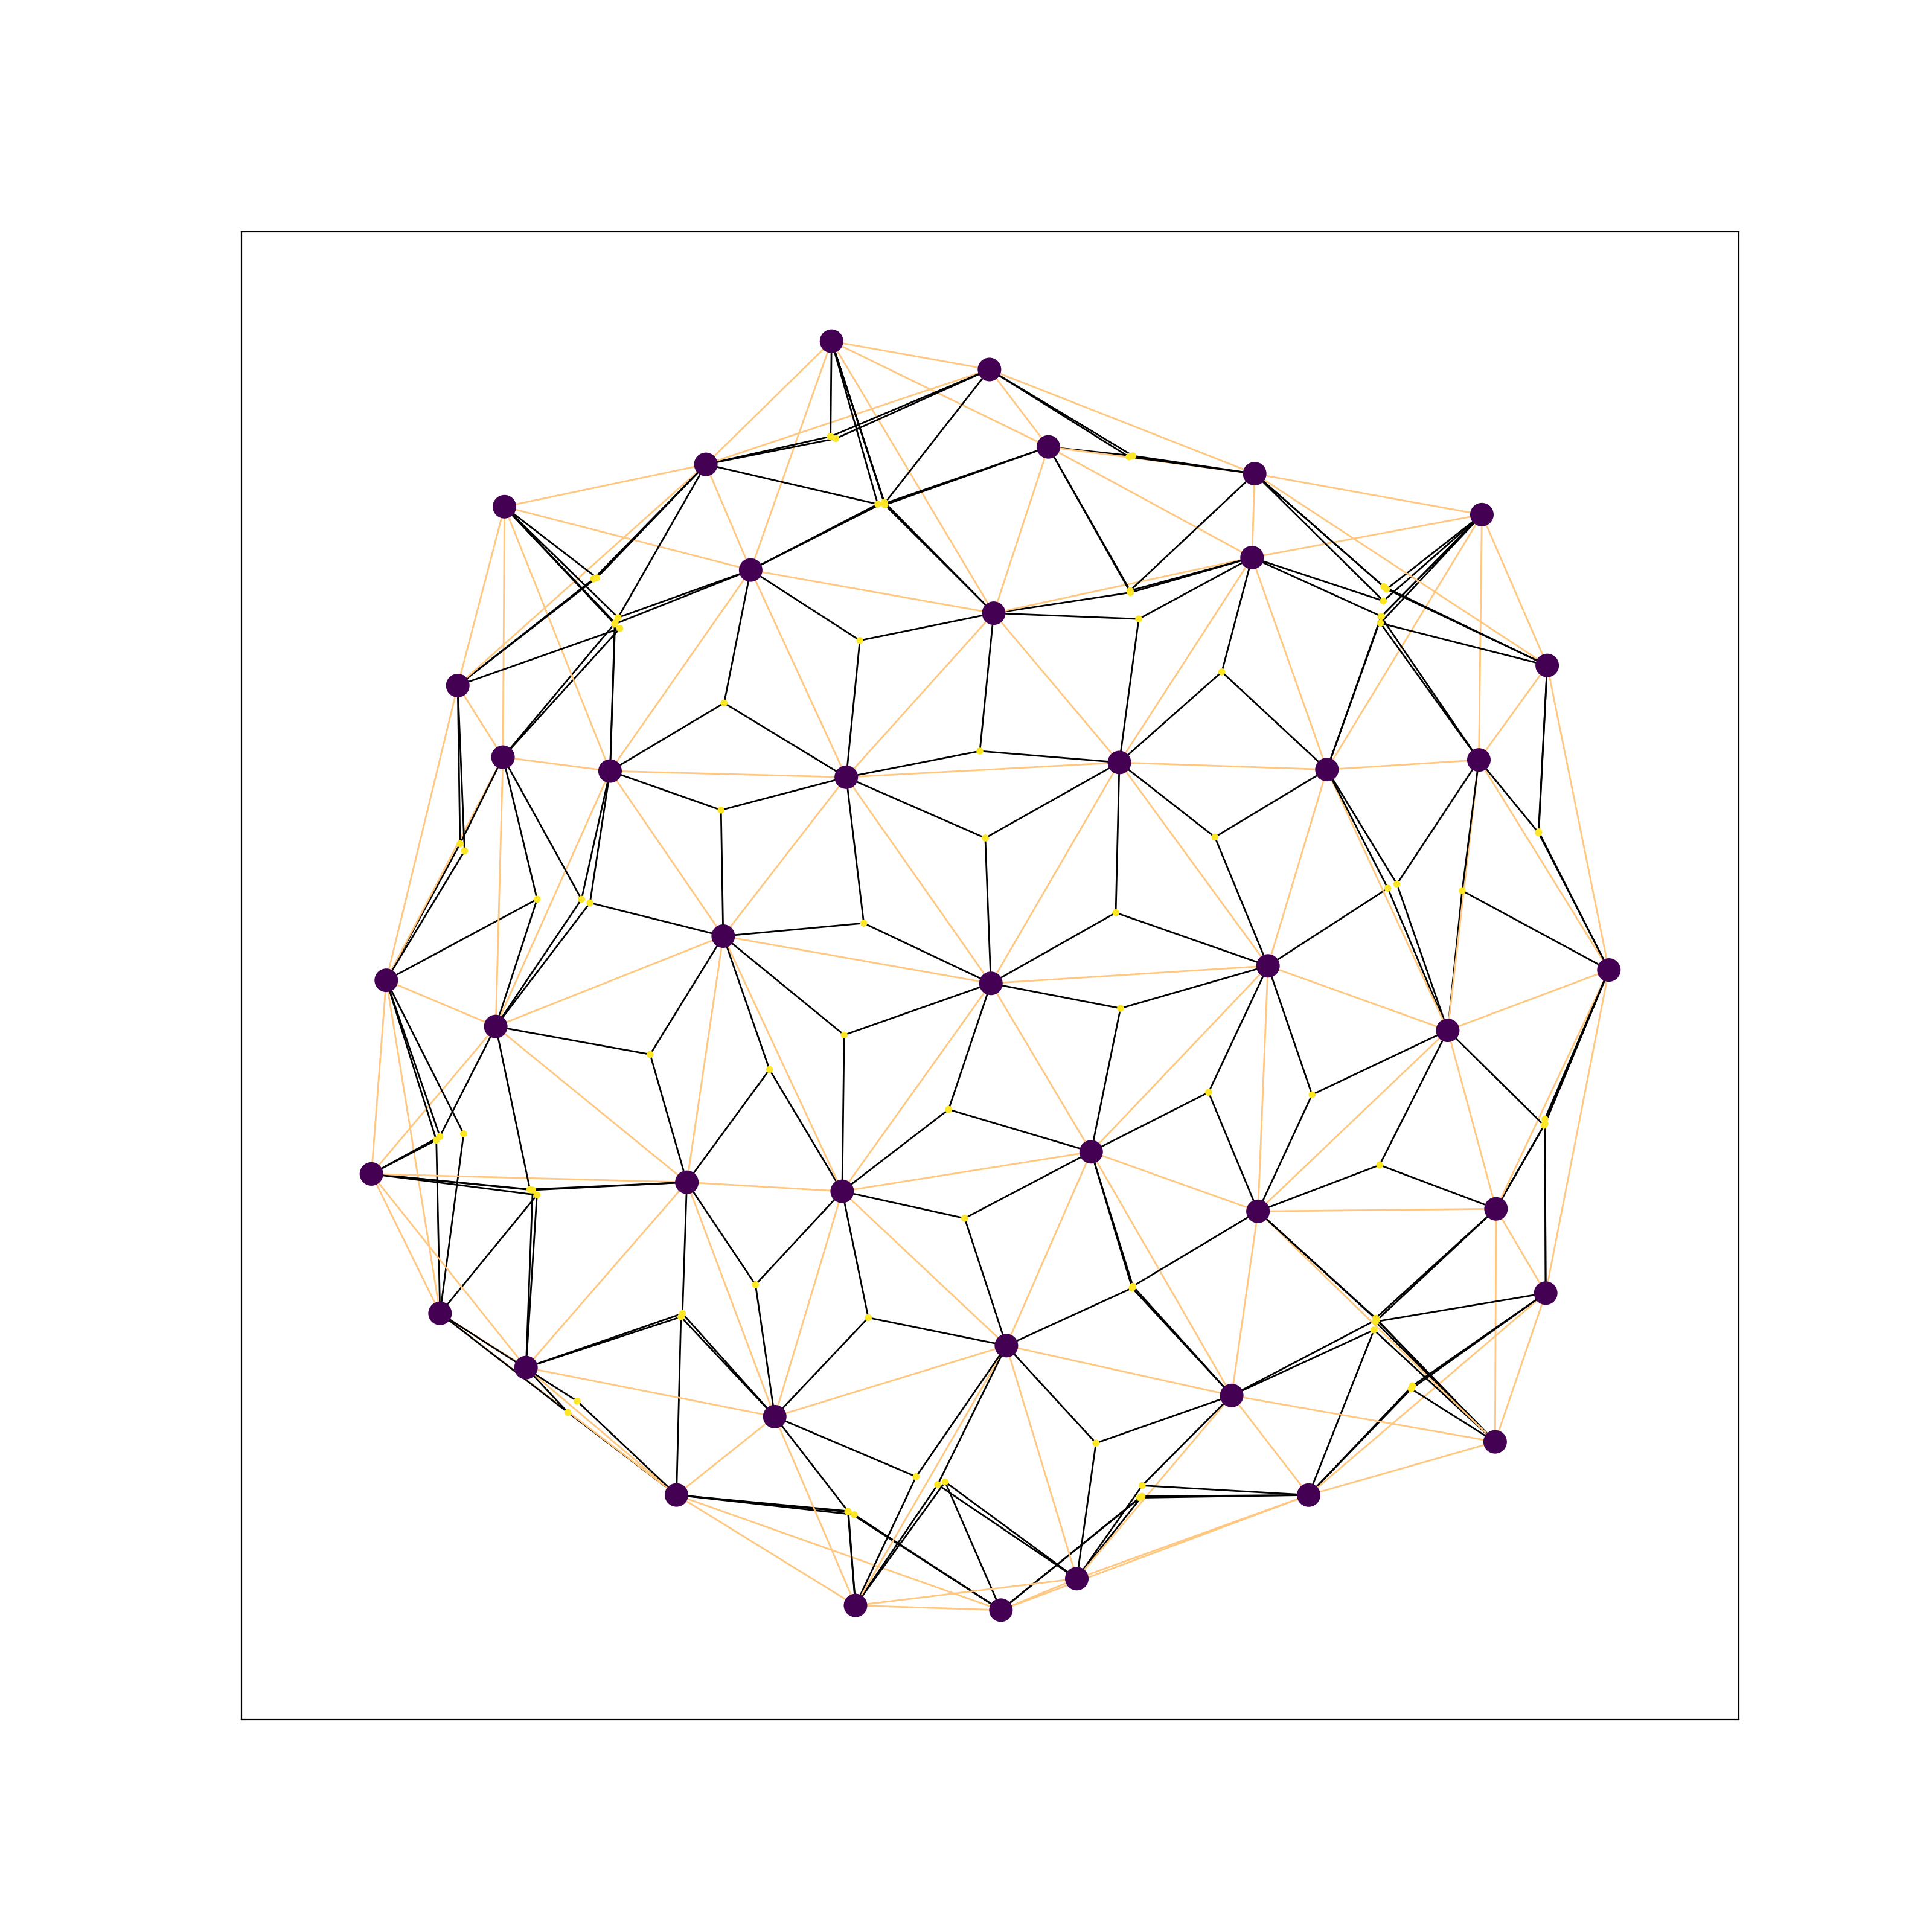
\includegraphics[width=0.3\textwidth]{hexbig/hexbig0.95_0.8_1.35_10_graph.png}
        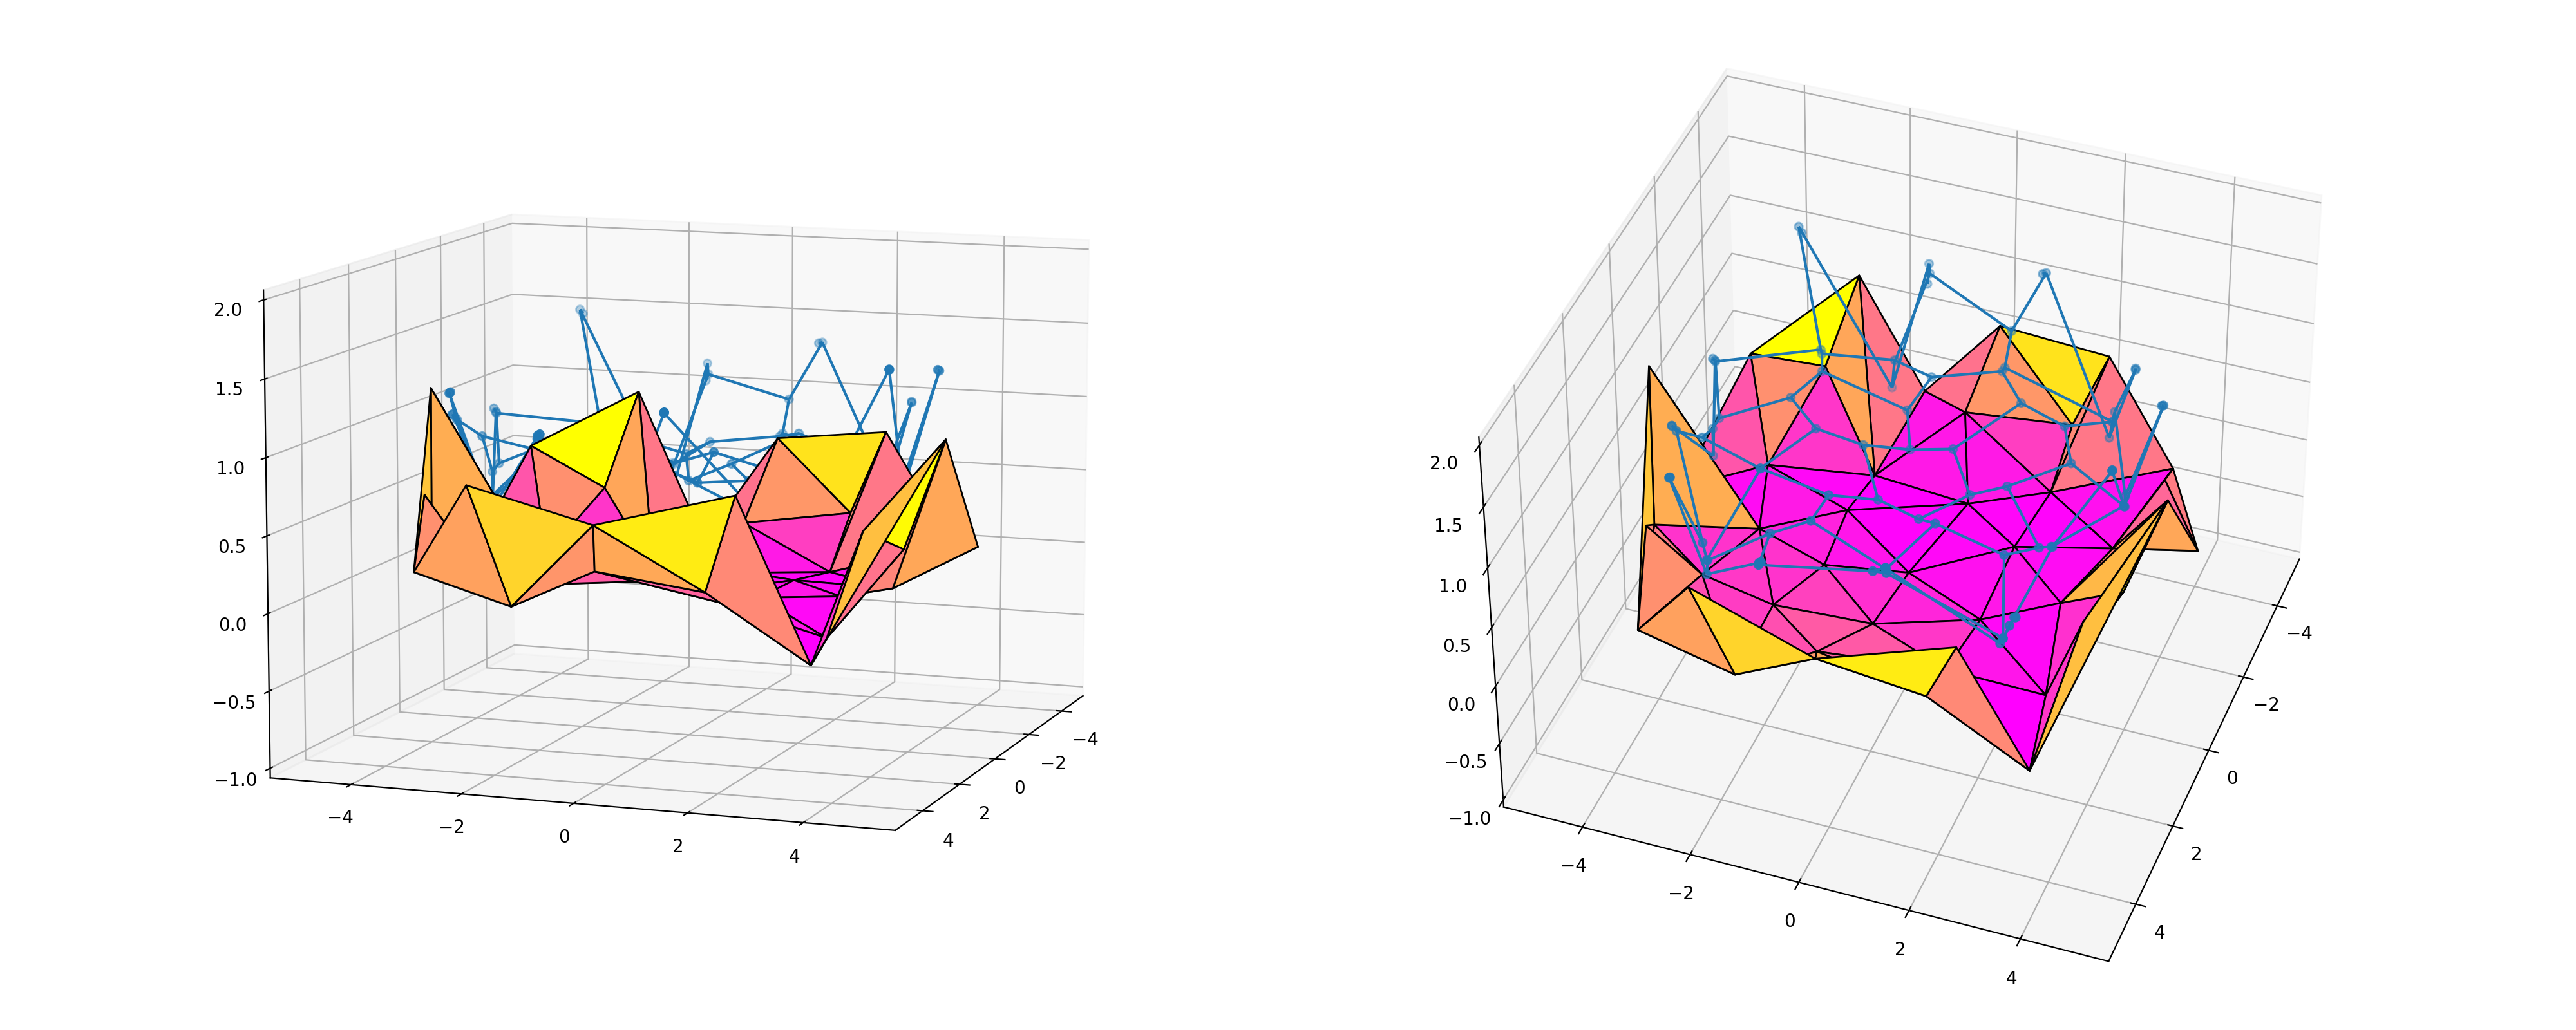
\includegraphics[width=0.69\textwidth]{hexbig/hexbig0.95_0.8_1.35_10_plot.png}
        \caption{Sheet shape when $\phi_0=0.95$, $\psi_0=0.8$, $\ell_0=1.52$.}
        \label{subfig:hexbig_out}
    \end{subfigure}
    \caption{Cell sheet geometry with a node of degree 7. The graph topology is affected in the sheet interior (subfigure \ref{subfig:hexbig_graph}). This minor change has substantial effects on the sheet geometry (subfigures \ref{subfig:hexbig_in}, \ref{subfig:hexbig_out}).}
    \label{fig:hexbig}
\end{figure}

\section{Varying the energy}



\begin{align*}
    \vec{F}_\gamma = \frac{\partial E}{\partial \vec{r}_\gamma} &= 2 \sum_{(\alpha, \rho)} \left( \phi_{(\alpha,\rho)} - \phi_0 \right) \frac{\partial \phi_{(\alpha,\rho)}}{\partial \vec{r}_\gamma} + 2 \sum_{(\alpha, \beta: \sigma, \rho)} \left( \psi(\hat{\bm{n}}_{\sigma\alpha\rho}, \hat{\bm{n}}_{\sigma\beta\rho}) - \psi_0 \right) \frac{\partial \psi_{(\alpha, \beta: \sigma, \rho)}}{\partial \vec{r}_\gamma} \\
    \frac{\partial \phi_{(\alpha,\rho)}}{\partial r_{\gamma i}} &= \frac{-1}{\sqrt{1 - (\hat{\bm{n}}_\alpha \cdot \hat{(\alpha\rho)})^2}} \left(\frac{\partial \hat{\bm{n}}_{\alpha j}}{\partial r_{\gamma i}} \hat{(\alpha\rho)}_j + \frac{\partial \hat{(\alpha\rho)}_j}{\partial r_{\gamma i}} \hat{\bm{n}}_{\alpha j} \right) \\
    \frac{\partial \hat{(\alpha\rho)}_j}{\partial r_{\gamma i}} &= \frac{(\delta_{\gamma\rho} - \delta_{\gamma\alpha})}{|r_\rho - r_\alpha|} \left( \delta_{ij} + \hat{(\alpha\rho)}_i\hat{(\alpha\rho)}_j \right) \\
    \frac{\partial \hat{\bm{n}}_{\alpha j}}{\partial r_{\gamma i}} &= \frac{\mathbb{1}_{\gamma\in \text{collars}(\alpha)} - n\delta_{\gamma\alpha}}{\left| \sum_{(\alpha, \rho)} (r_\rho - r_\alpha) \right|} \left(\delta_{ij} - \hat{\bm{n}}_{\alpha i} \hat{\bm{n}}_{\alpha j} \right) \\
    \frac{\partial \psi_{(\alpha, \beta: \sigma, \rho)}}{\partial r_{\gamma i}} &= \frac{-1}{\sqrt{1 - (\hat{\bm{n}}_{\rho\alpha\sigma} \cdot \hat{\bm{n}}_{\rho\beta\sigma}})^2} \left(\frac{\partial \hat{\bm{n}}_{\rho\alpha\sigma j}}{\partial r_{\gamma i}} \hat{\bm{n}}_{\rho\beta\sigma j} + \frac{\partial \hat{\bm{n}}_{\rho\beta\sigma j}}{\partial r_{\gamma i}} \hat{\bm{n}}_{\rho\alpha\sigma j} \right) \\
    \frac{\partial \hat{\bm{n}}_{\rho\alpha\sigma j}}{\partial r_{\gamma i}} &= \text{too big see notes}
\end{align*}
